\documentclass{article}

% ------------------------------------------------------------ %
% packages
%
\usepackage{amsmath}
\usepackage{authblk} % for affiliations
\renewcommand\Affilfont{\itshape\footnotesize}
\setlength{\affilsep}{1em}

\usepackage{graphicx} 
\pagenumbering{gobble}
\usepackage{caption}
\usepackage{subcaption}
\usepackage{geometry}
\geometry{
	a4paper,
	total={170mm,257mm},
	left=20mm,
	top=15mm,
}
\usepackage[hidelinks=TRUE]{hyperref}
% to position last two rows at top of page2
\makeatletter
\setlength{\@fptop}{0pt}
\makeatother


% enhanced tables
\usepackage{multicol}              
\usepackage{multirow}
\usepackage{booktabs} 
\usepackage{geometry}
\usepackage[UKenglish]{isodate}
\cleanlookdateon

\usepackage[ttscale=.875]{libertine} % change style
\usepackage{lineno}
% adjust caption properties
\usepackage[margin=10pt, font=small, labelfont=bf, tableposition=top]{caption}

\frenchspacing
% ------------------------------------------------------------ %
% additional information
\author[]{Severin Hauenstein}
\affil[]{Department of Biometry and Environmental System Analysis, University of Freiburg, 79106 Freiburg, Germany}
%
\title{Data simulation in ecological research: Spatial autocorrelation}
% ------------------------------------------------------------ %

\begin{document}
\maketitle
\section{Data simulation with \textsf{simSAC}}
The data simulated with \textsf{simSAC} can be varied in predictor landscape, distribution of the response variable and cause of spatial autocorrelation (SAC). The three predictor landscapes are linear and non-linear gradients without noise (``smooth"), unconditional Gaussian random fields from an exponential covariance model (``realistic"), and ``real" bio-climatic data from \url{http://www.worldclim.org} (see fig.~\ref{predictor_maps}). 
The response distribution can be Gaussian, Bernoulli or zero-inflated Poisson. Spatial autocorrelation was caused by adding SAC onto the response variable, omitting an important predictor in the model, the wrong functional form of the model (i.e. the model must miss a quadratic term or interaction) or dispersal (i.e. smoothing out values/ probabilities). The full number of datasets is 45.\\

Here we choose a minimal set of 12 =  2 landscapes * 2 distributions * 3 SAC causes (see table~\ref{minimalset}).
For the data with a smooth \textbf{landscape} the seven predictors are: 
\begin{itemize}
	\setlength\itemsep{-0.2em}
	\item $x_1 = lon$
	\item $x_2 = lat$
	\item $x_3 = (lon - \overline{lon})^2$
	\item $x_4 = (lat - \overline{lat})^2$
	\item $x_5 = x_3^{x_4}x_4^{x_3}$
	\item $x_6 = x_1^{x_1}x_3^{x_4}$
	\item $x_7 = x_2^{x_1}x_4^{x_3}log(x_5 + 1))$
\end{itemize}
where $lon$ and $lat$ are (simulated) longitude and latitude. As for the data with real landscapes seven real bio-climatic predictors are cropped to the extent of 5N24E to 7S37E. The bio-climatic variables are: 
\begin{itemize}
	\setlength\itemsep{-0.2em}
	\item $x_1 =$ annual mean temperature
	\item $x_2 =$ precipitation of coldest quarter
	\item $x_3 =$ mean diurnal range
	\item $x_4 =$ annual precipitation
	\item $x_5 =$ temperature seasonality
	\item $x_6 =$ precipitation of warmest quarter
	\item $x_7 =$ isothermality
\end{itemize}
Regardless of the landscape, all predictors are rescaled to [-1,1].\\

The Gaussian  \textbf{response distribution} is simulated as $y \sim \mathcal{N}(\beta_0 + \beta_1x_1 + \beta_2x_4 + \beta_3x_4^2 + \beta_4x_3*x_4 + \beta_5x_3, \sigma=0.2)$ with $\beta$-values of 0.8, 0.2, -0.9, 0.8, -0.6 and 0.5, respectively.
As for the Bernoulli distribution $y \sim \textrm{Bern}(\textrm{logit}^{-1}(\beta_0 + \beta_1x_1 + \beta_2x_4 + \beta_3x_4^2 + \beta_4x_3*x_4 + \beta_5x_3))$, with $\beta$-values of 0.2, 4.5, -1.2, -1.2, -1.1 and 0.9, respectively.\\
 
We impose five different \textbf{autocorrelation regimes}. of which we use three in the minimal set:
\begin{description}
	\setlength\itemsep{-0.2em}
	\item[SAC cause 0] The response variable without spatial autocorrelation is used as reference scenario.
	\item[SAC cause 1] Adding spatial autocorrelation onto the response variable. We first compute the correlation structure as $\Omega = e^{-0.3D}$, where $D$ is the euclidean distance matrix. By computing the inverse of the Choleski decomposition of $\Omega$ we obtain the correlation weights matrix ($w=Chol(\Omega)^{-1}$). We then preform a matrix multiplication of $w^{-1}$ with $n$ values drawn from $\mathcal{N}(\mu=0, \sigma=0)$, where $n=$ is the number of rows of $D$.
	\item[SAC cause 2] Omitting $x_1$ as important predictor
\end{description}

Fig.~\ref{checkSAC} shows the response and residuals (from a linear model) maps and correlograms for the five different spatial autocorrelation scenarios. For the latter the spatial dependence measure is Moran's I.




\begin{table}[b!]
	\centering
	\caption{12 datasets (=  2 landscapes * 2 distributions * 3 SAC) causes as minimal set of simulated data.\label{minimalset}}
	\begin{tabular}{clll}
		\toprule
		dataset & landscape & distribution & SAC cause\\
		\midrule
		110 & smooth & Gaussian & reference\\
		111 & & & SAC onto response variable\\
		112 & & & omitted predictor\\
		120 & & Bernoulli & reference\\
		121 & & & SAC onto response variable\\
		122 & & & omitted predictor\\
		310 & real & Gaussian & reference\\
		311 & & & SAC onto response variable\\
		312 & & & omitted predictor\\
		320 & & Bernoulli & reference\\
		321 & & & SAC onto response variable\\
		322 & & & omitted predictor\\
		\bottomrule
	\end{tabular}
\end{table}  
	
\begin{figure}
 	\begin{subfigure}{0.3\textwidth}
 		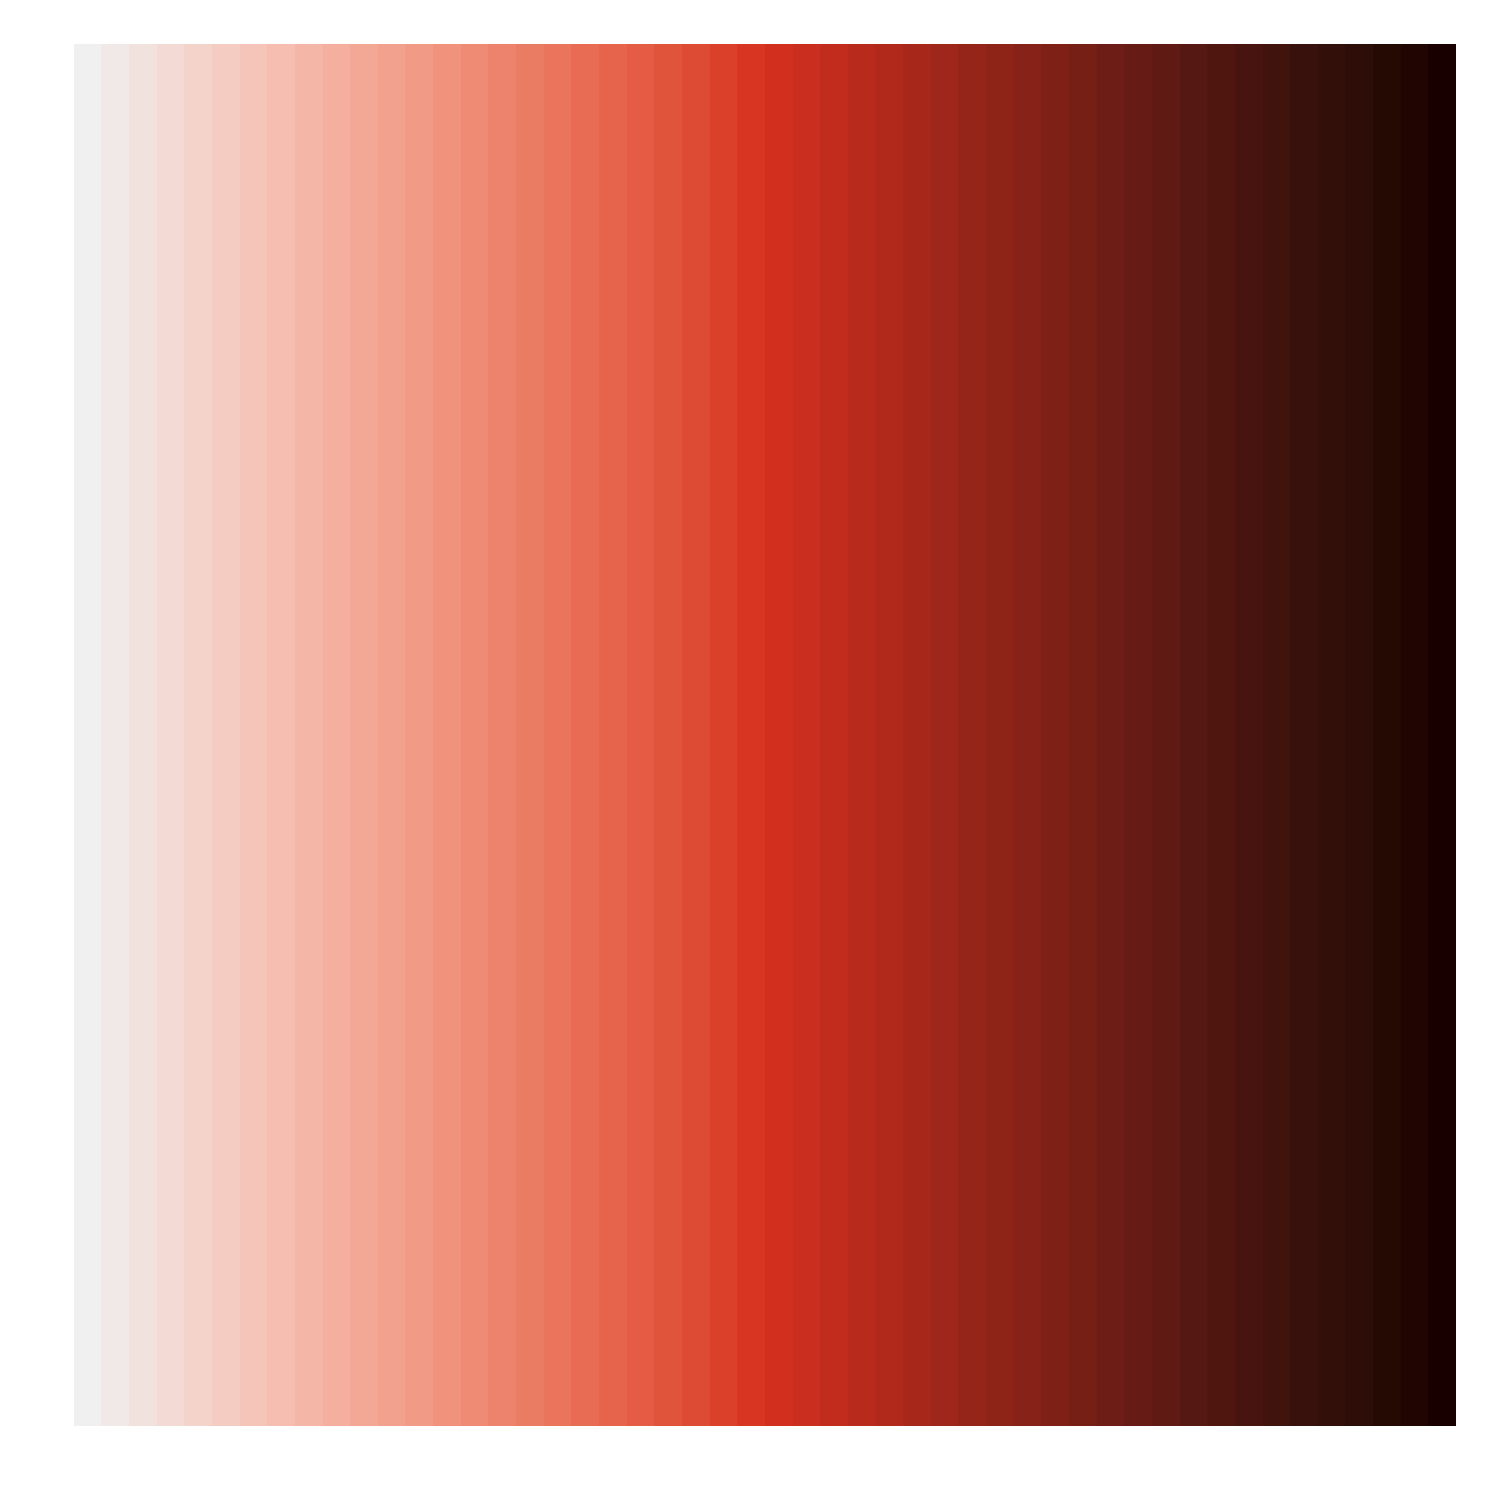
\includegraphics[width=\linewidth]{figures/p_smooth1}\\
 		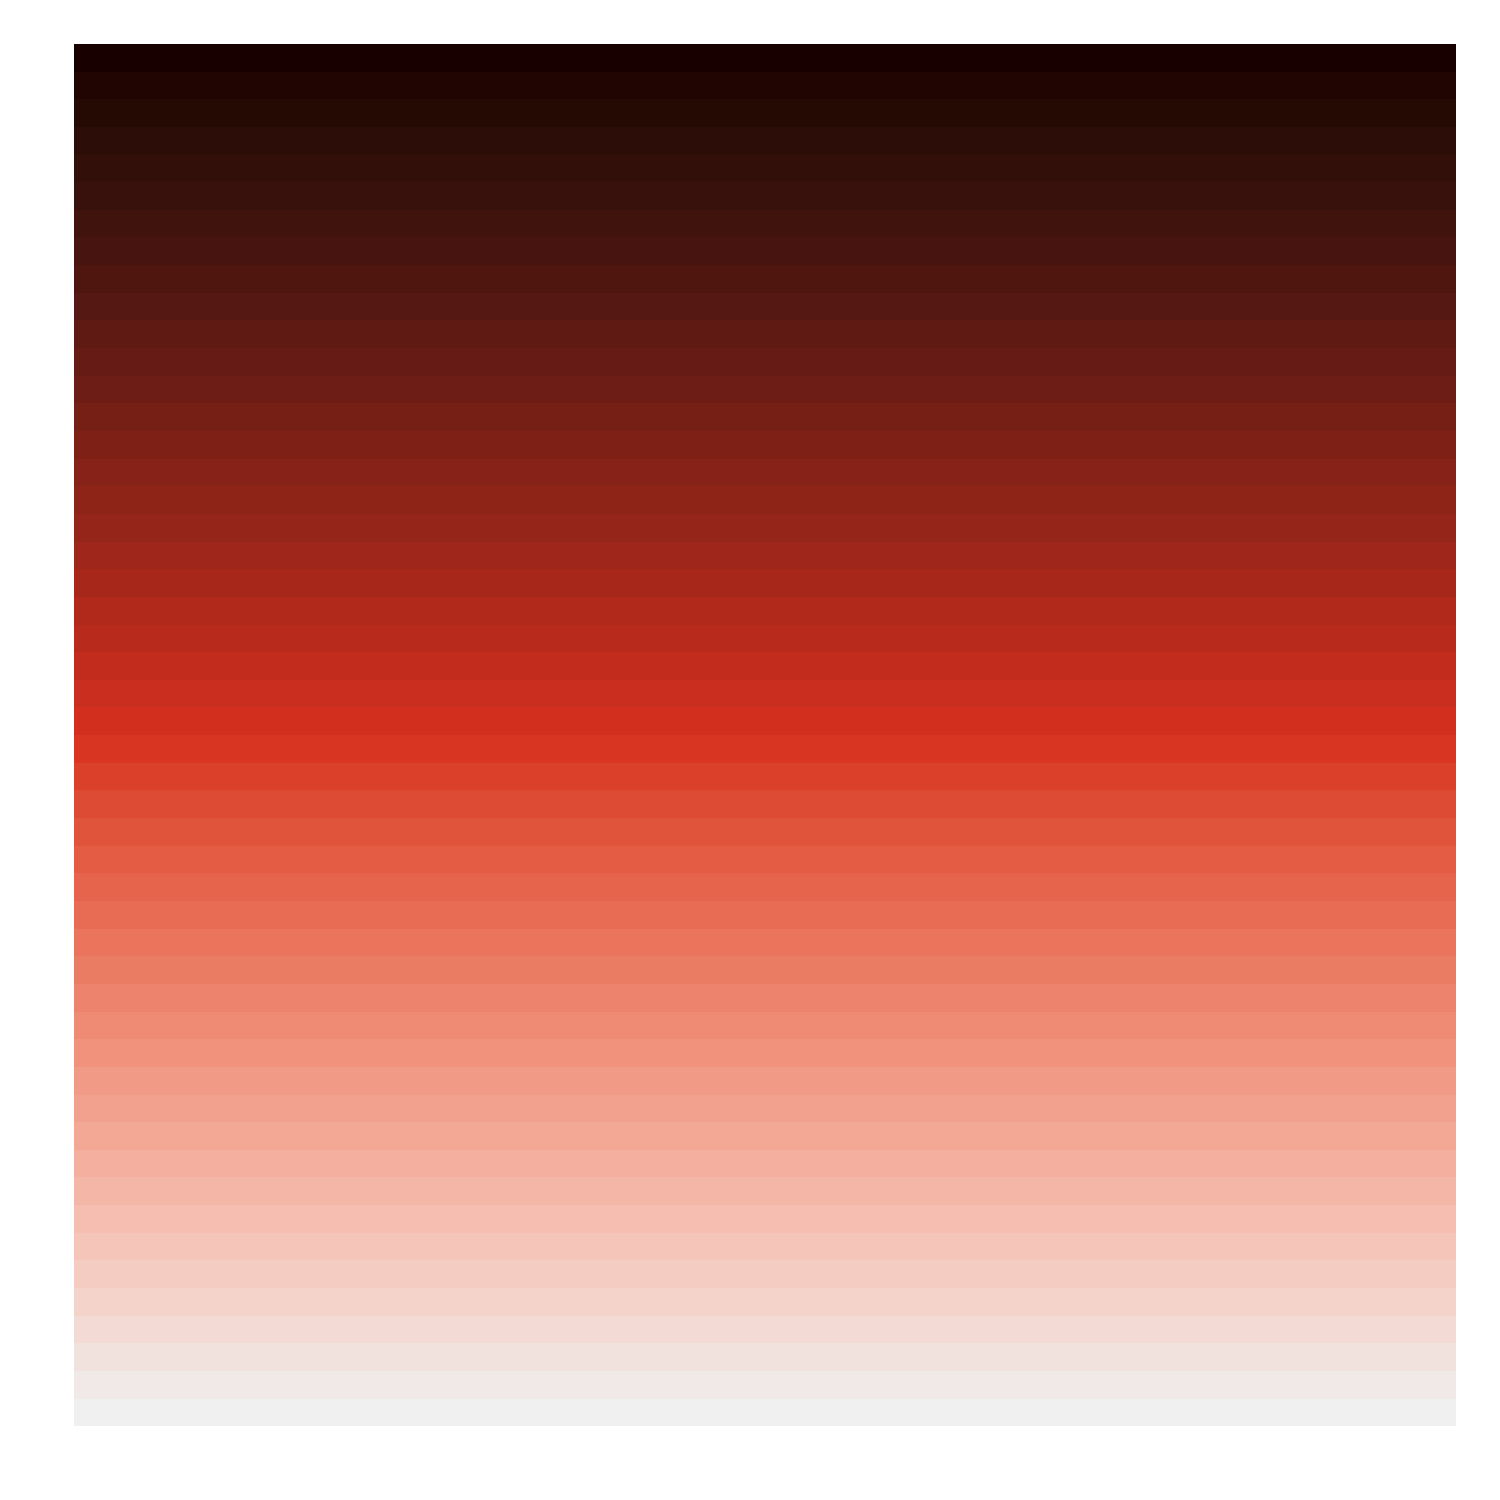
\includegraphics[width=\linewidth]{figures/p_smooth2}\\
 		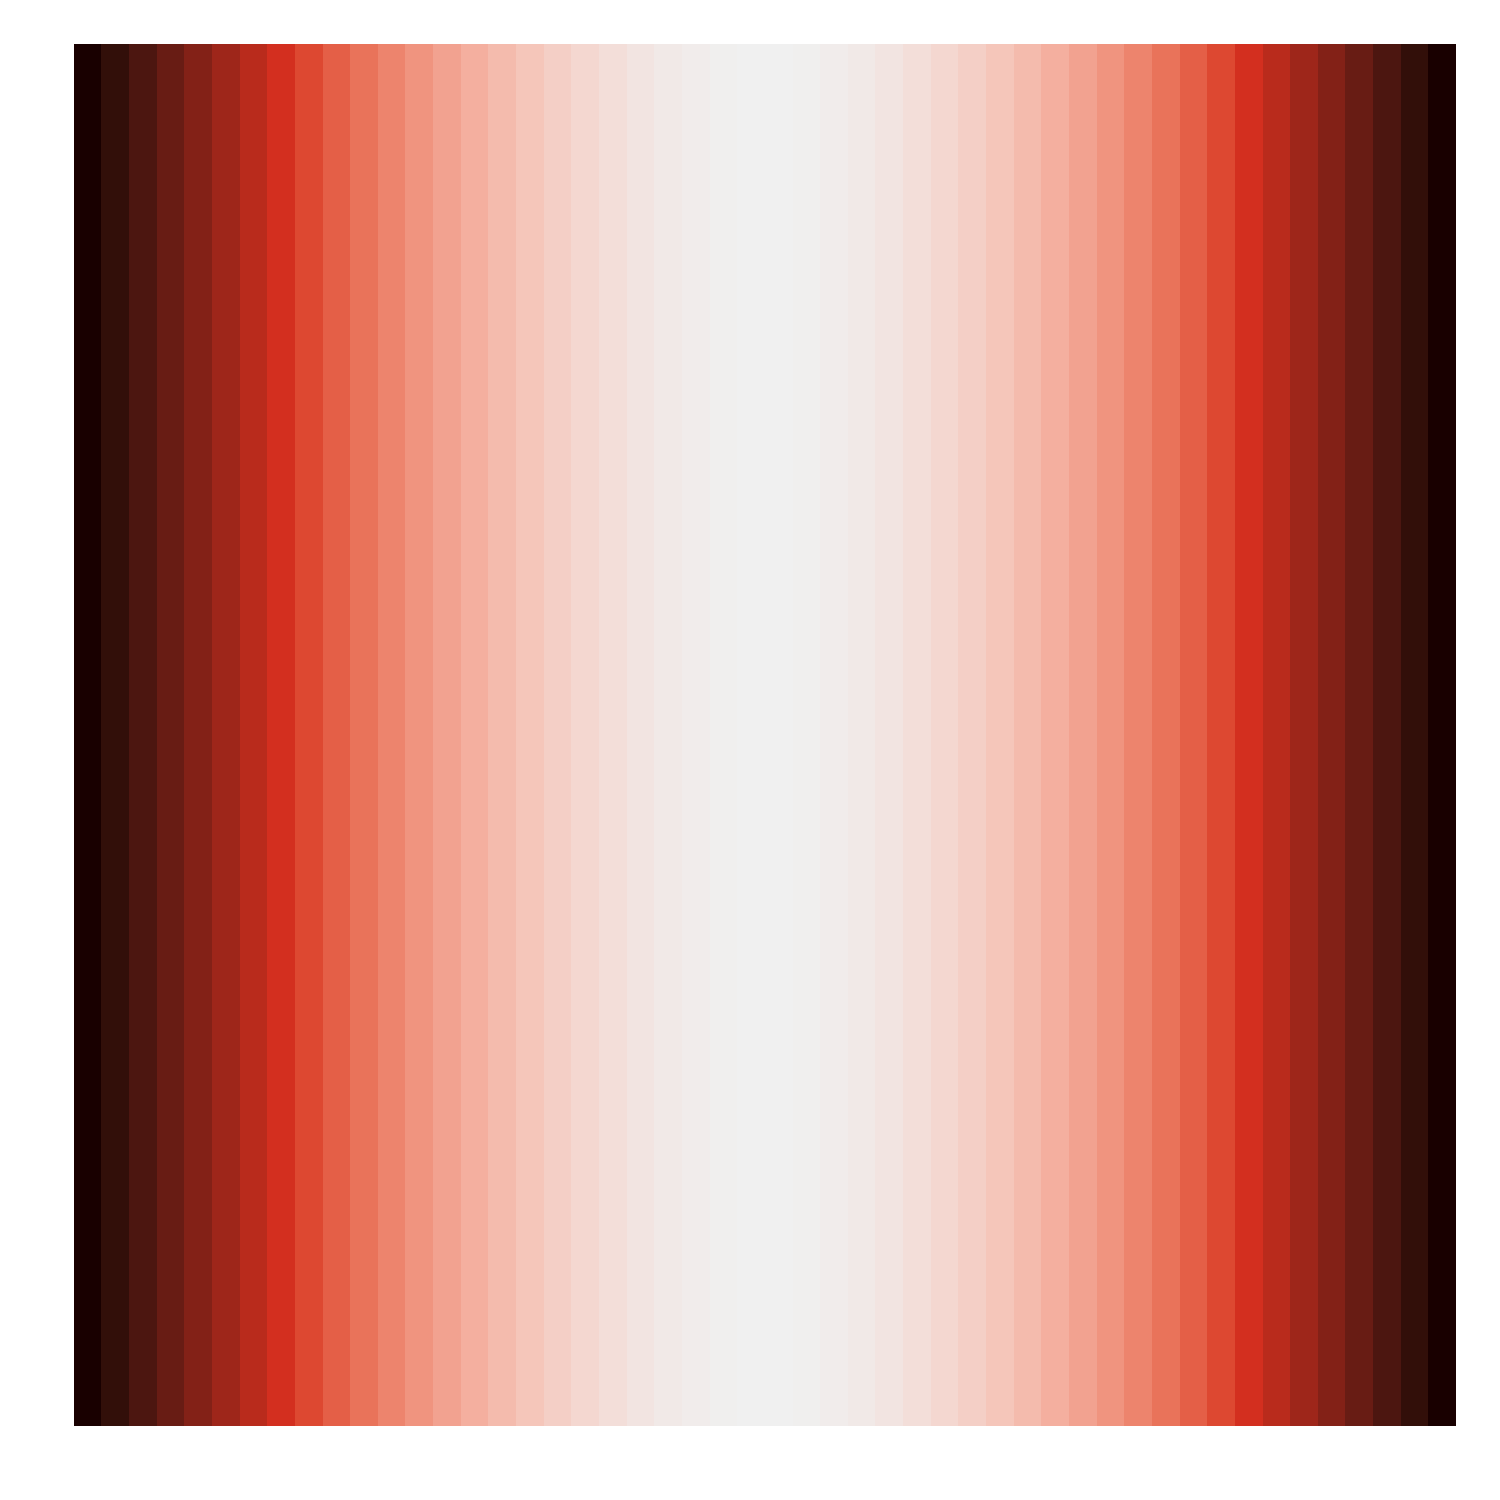
\includegraphics[width=\linewidth]{figures/p_smooth3}\\
 		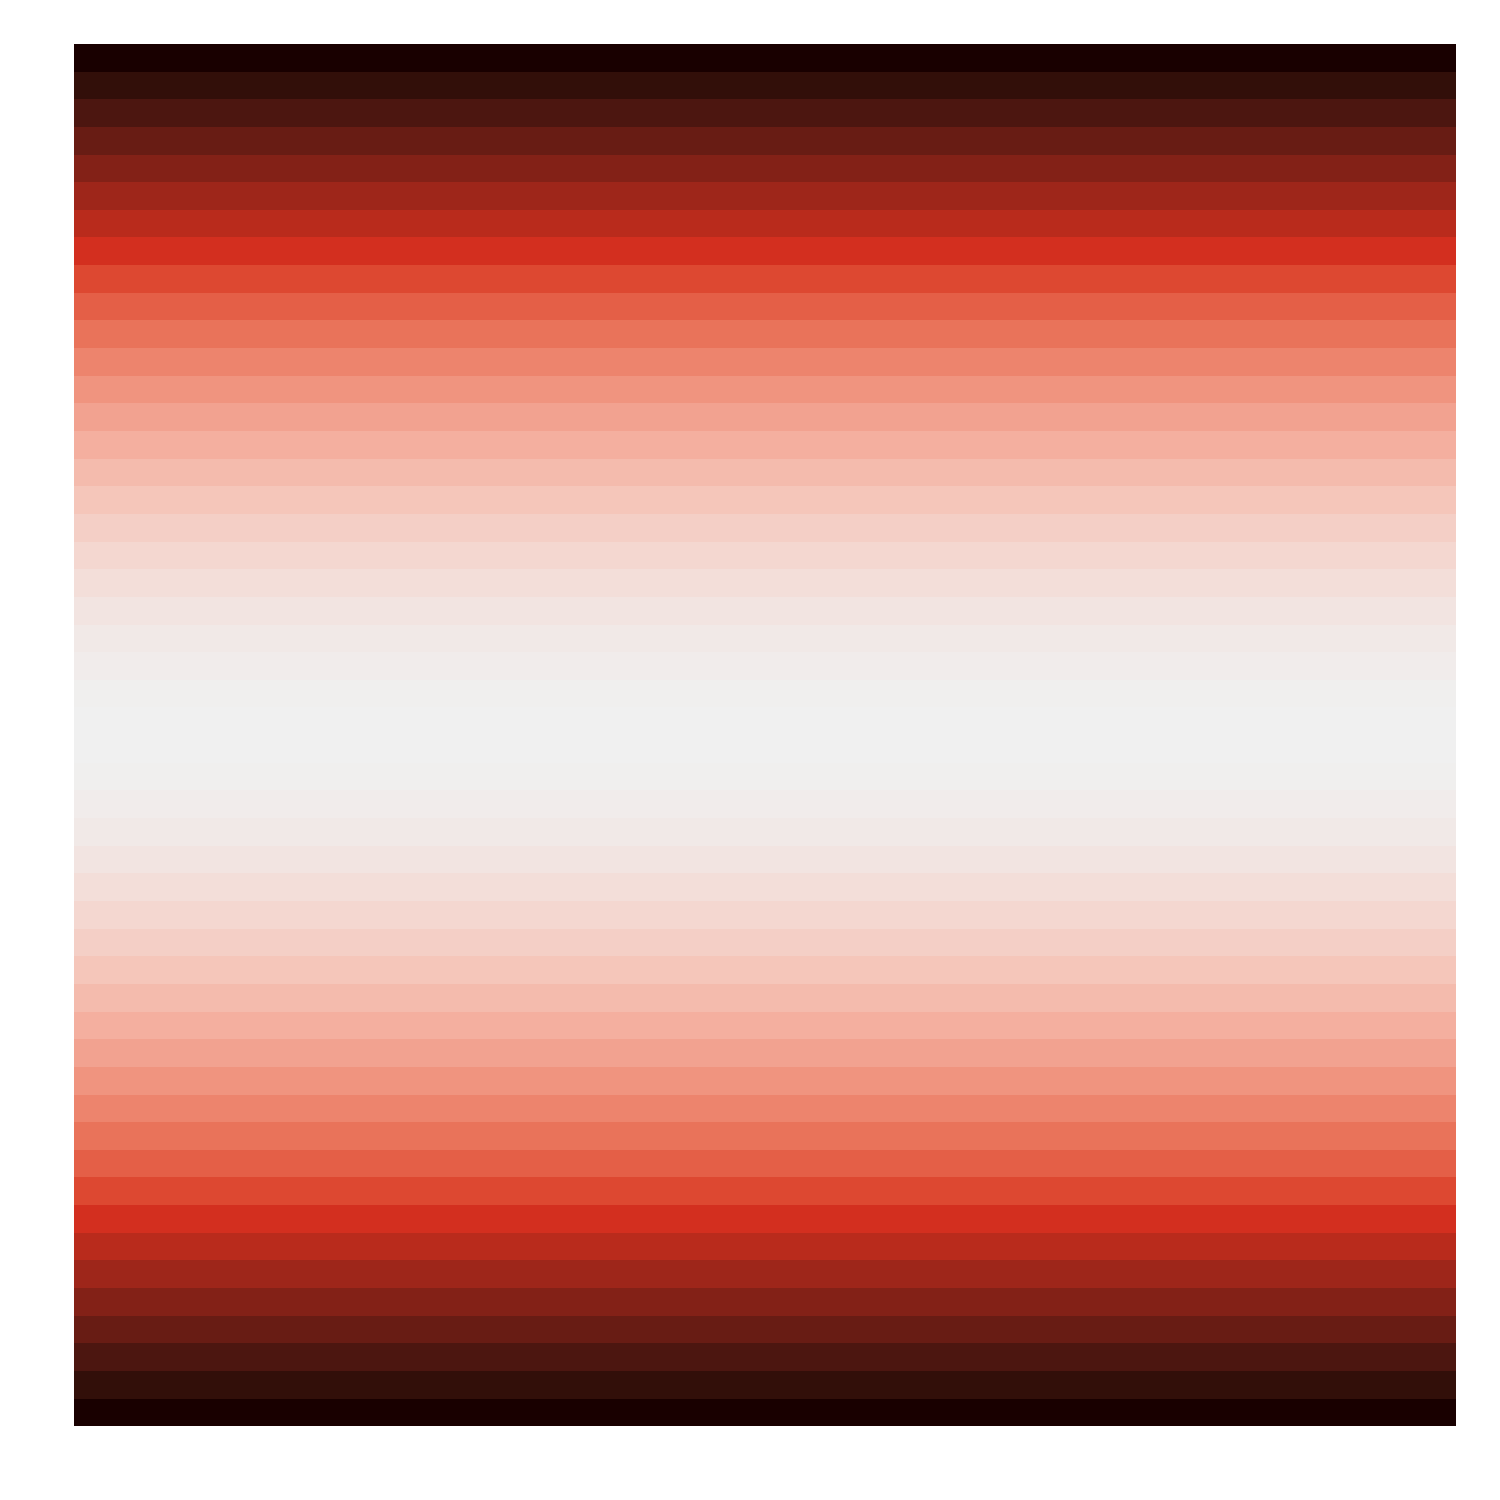
\includegraphics[width=\linewidth]{figures/p_smooth4}\\
 		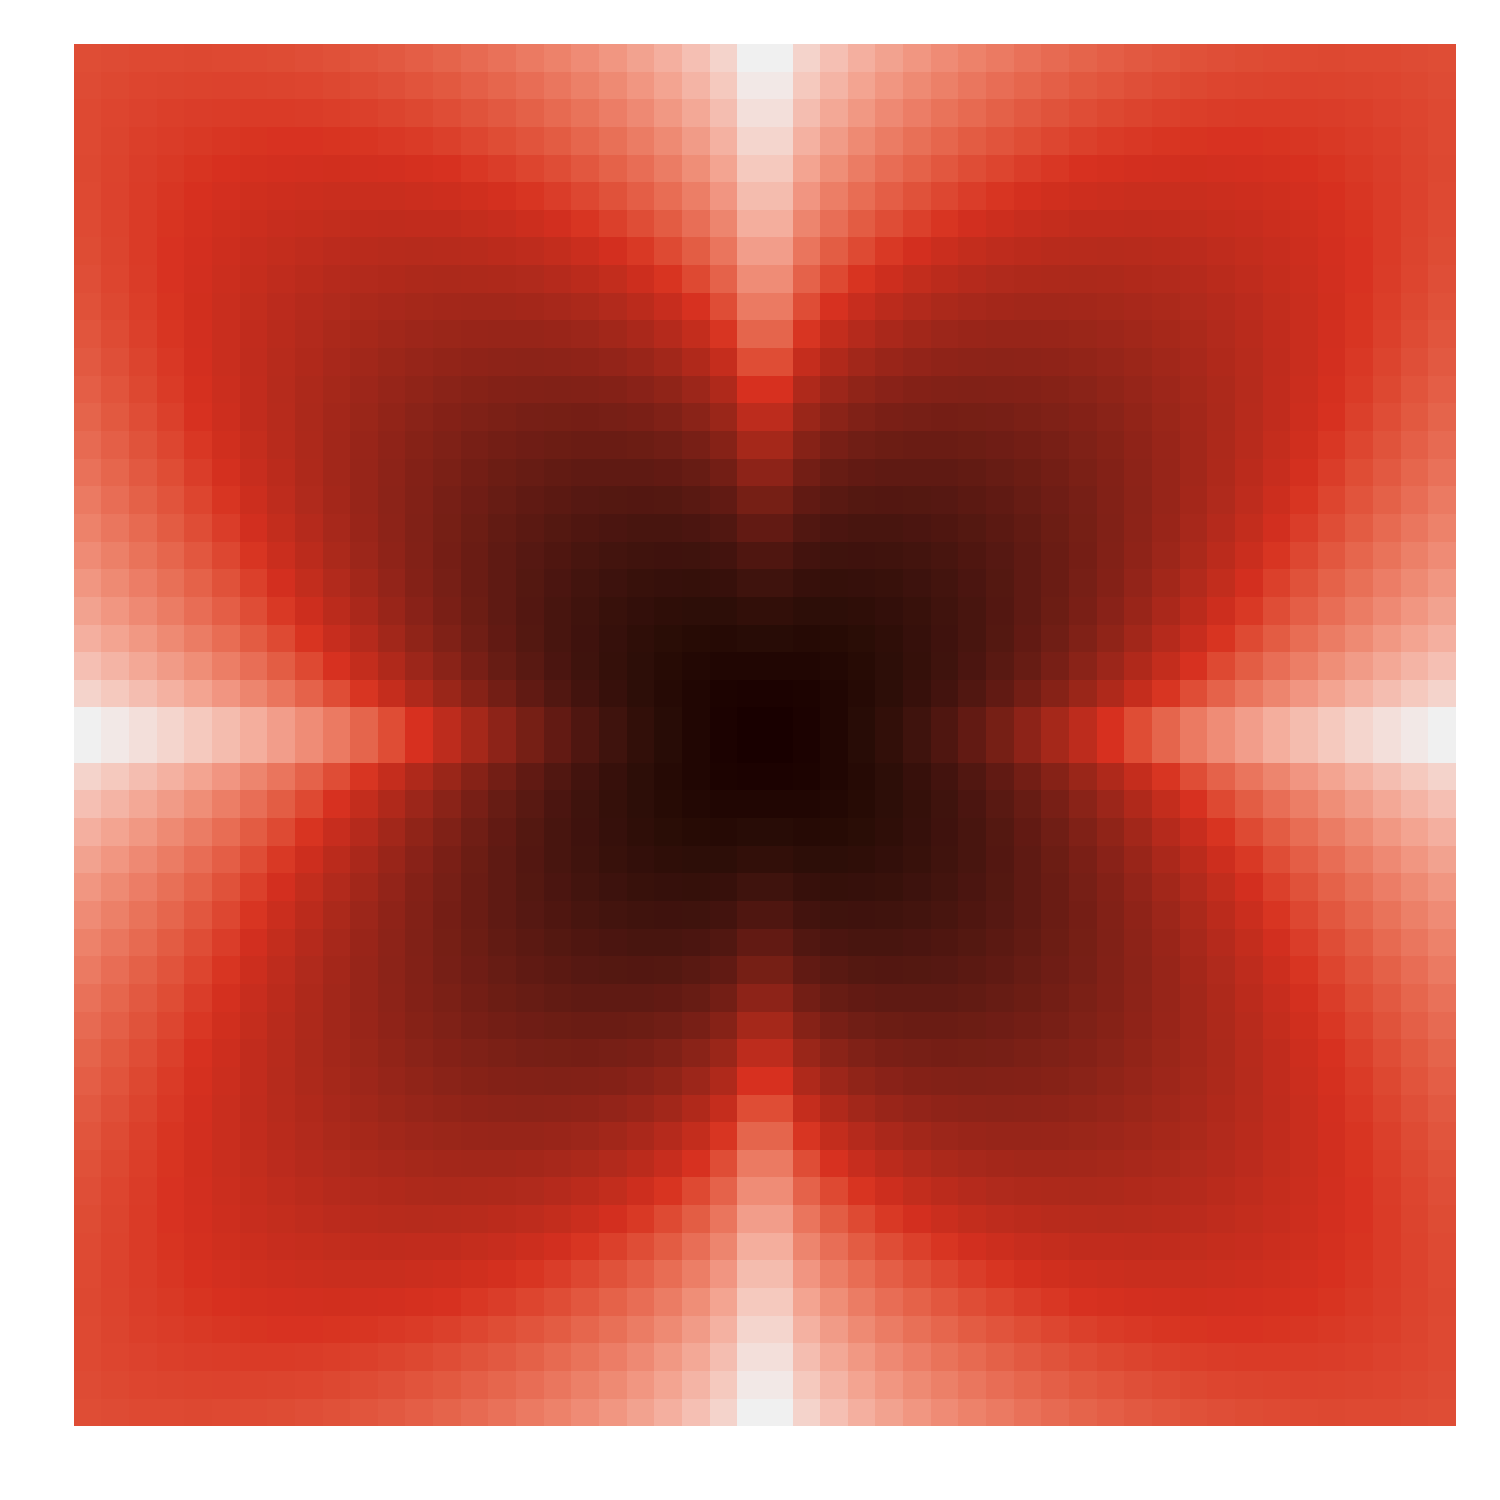
\includegraphics[width=\linewidth]{figures/p_smooth5}\\
 		%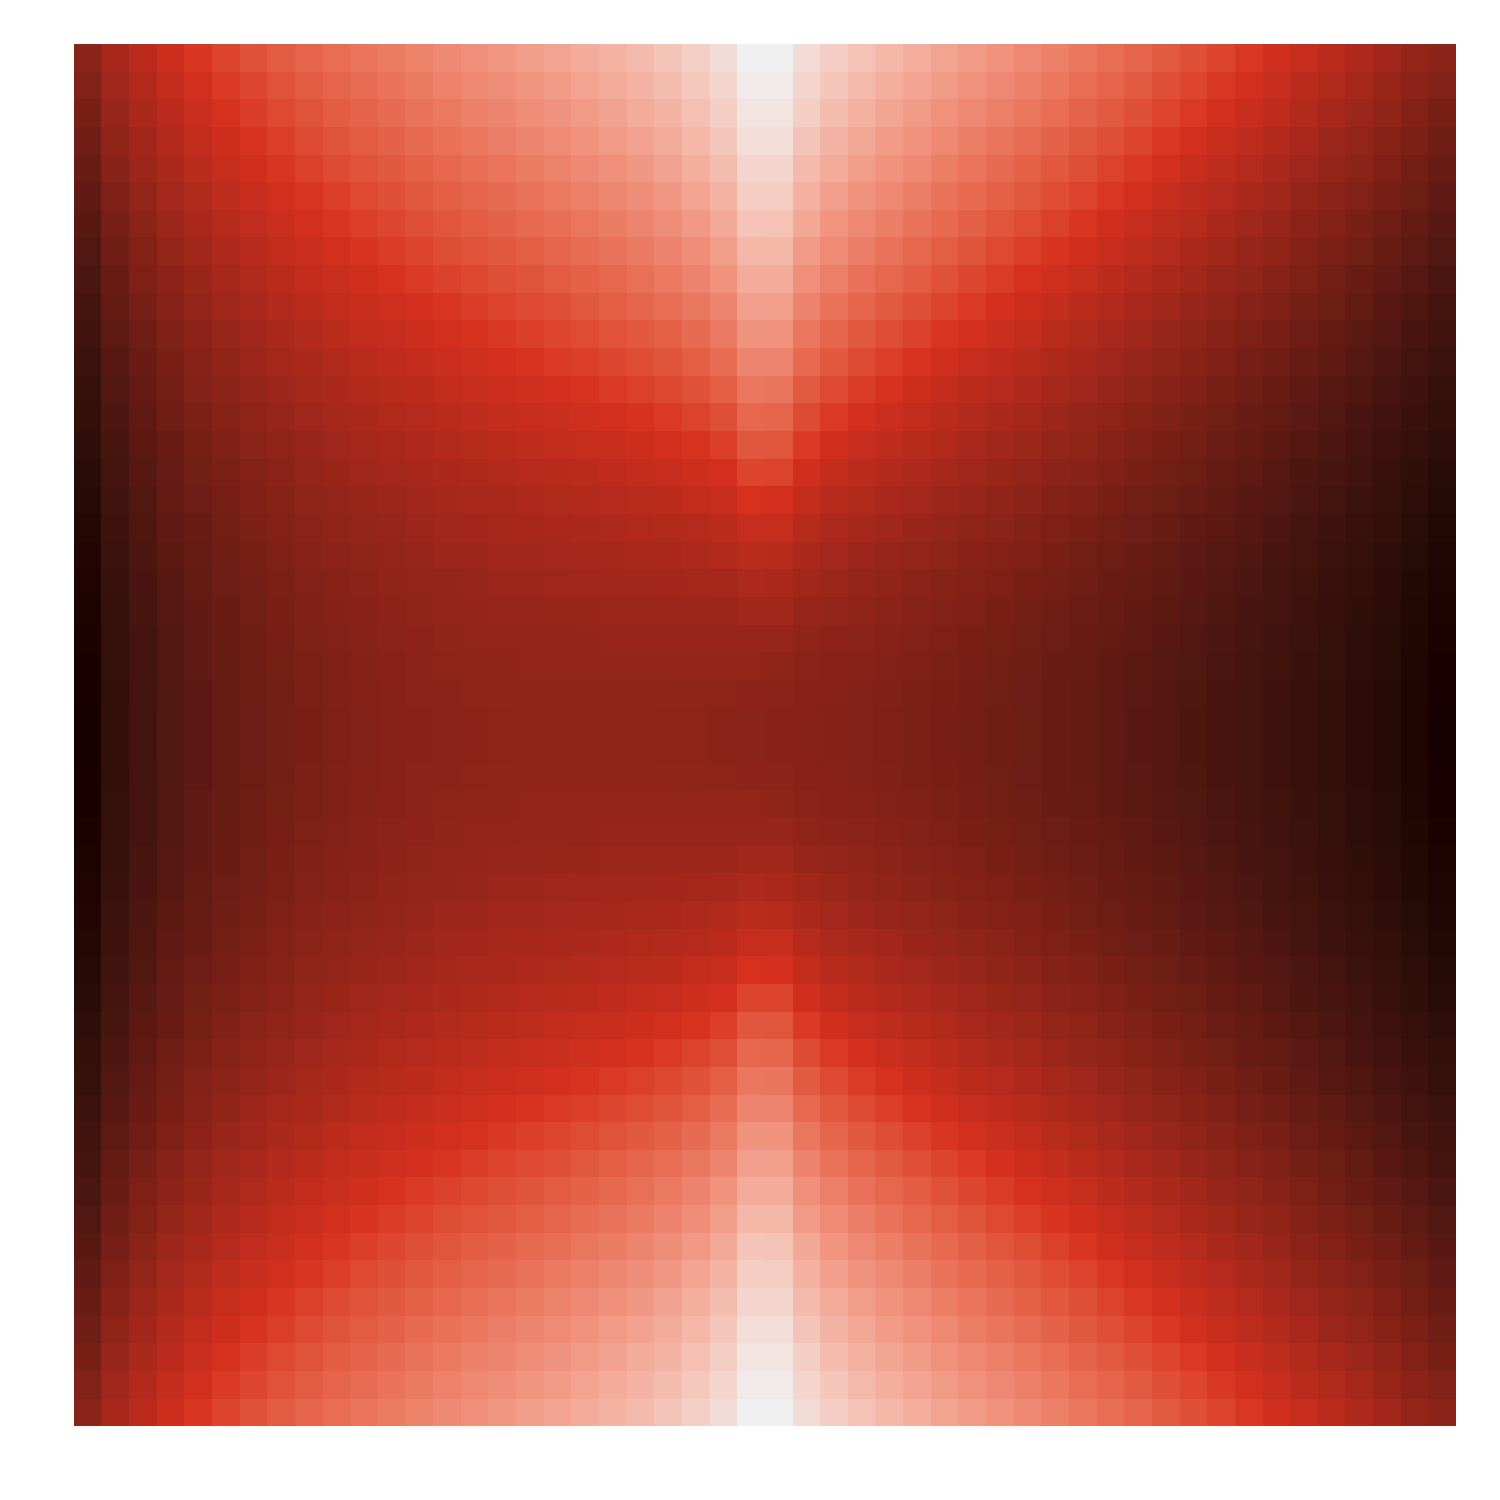
\includegraphics[width=\linewidth]{figures/p_smooth6}\\
 		%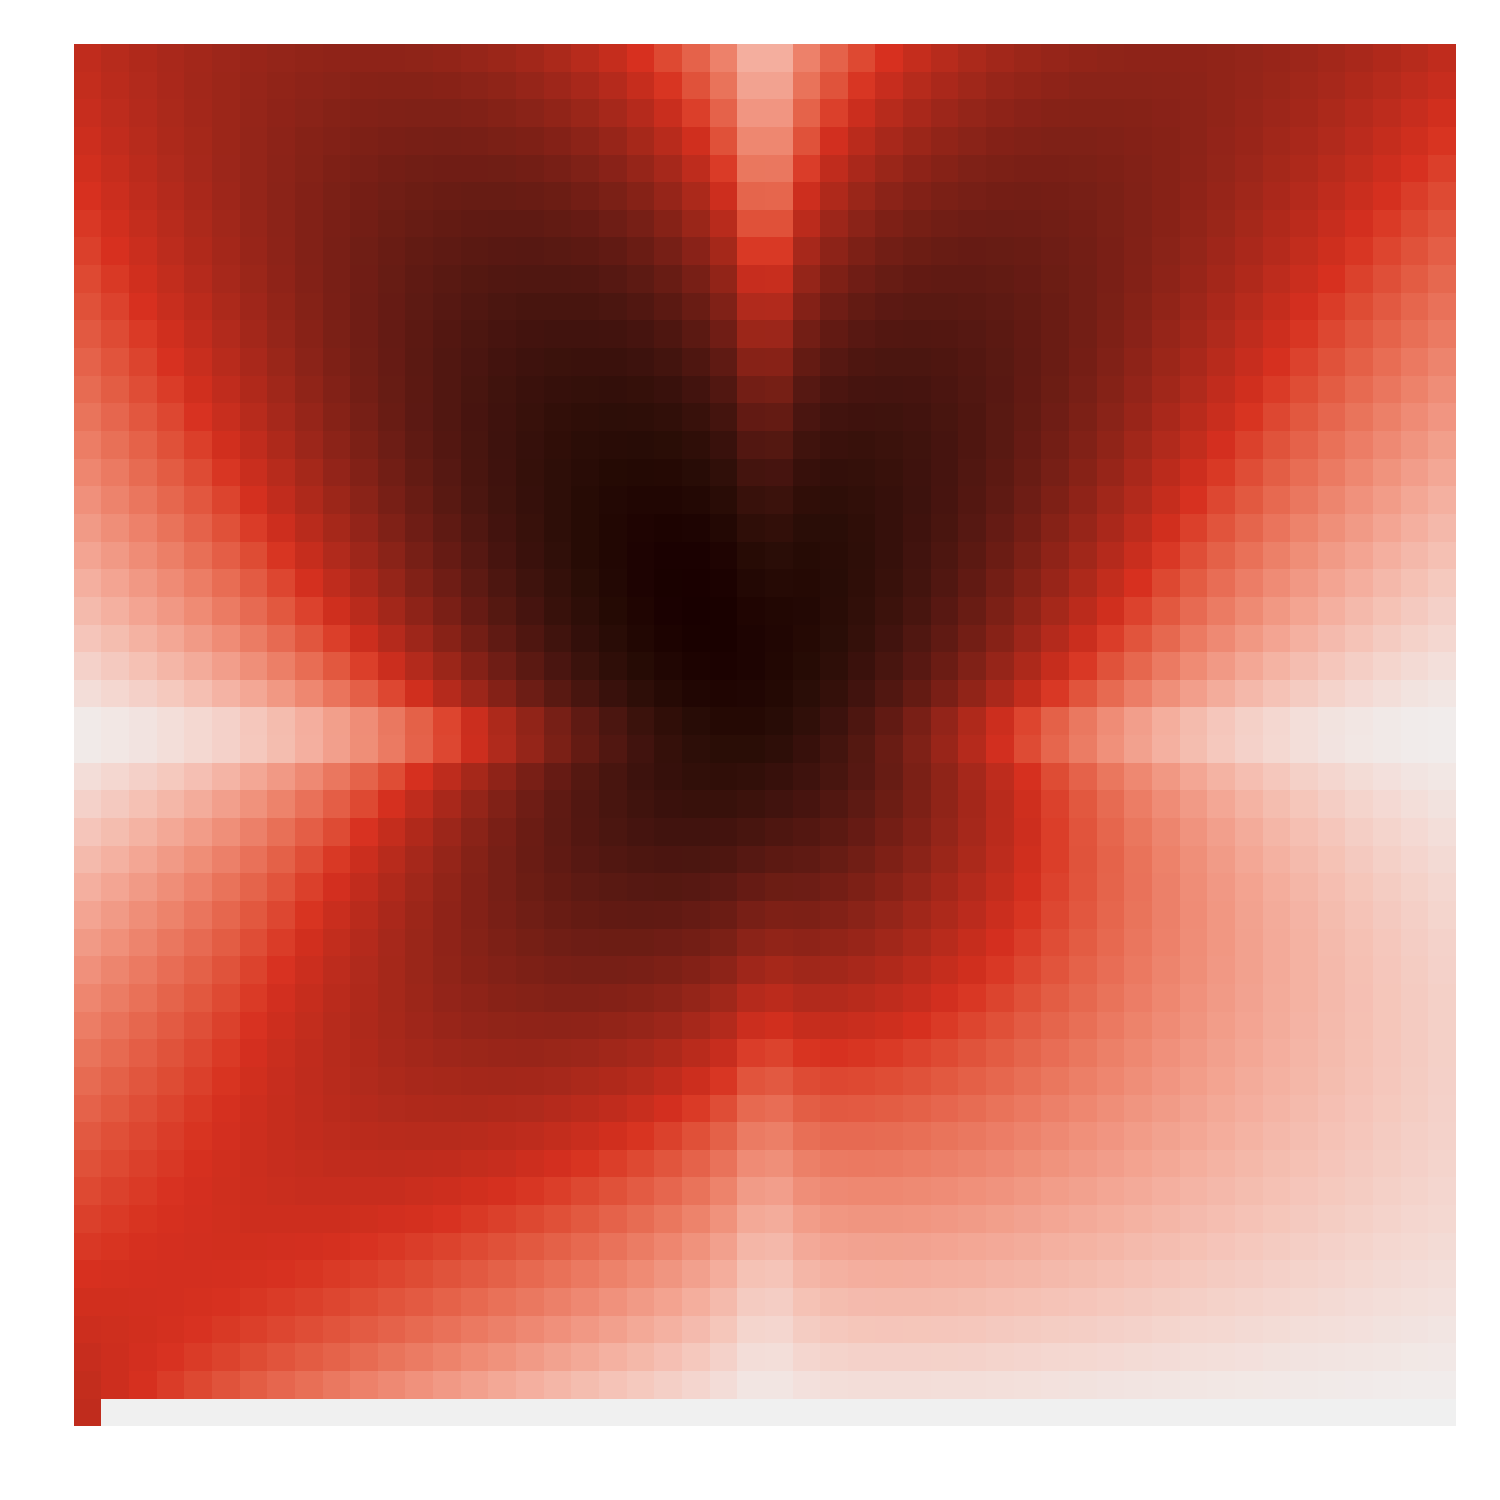
\includegraphics[width=\linewidth]{figures/p_smooth7}\\
 		%\caption{First}
 	\end{subfigure}
 	\begin{subfigure}{0.3\textwidth}
 		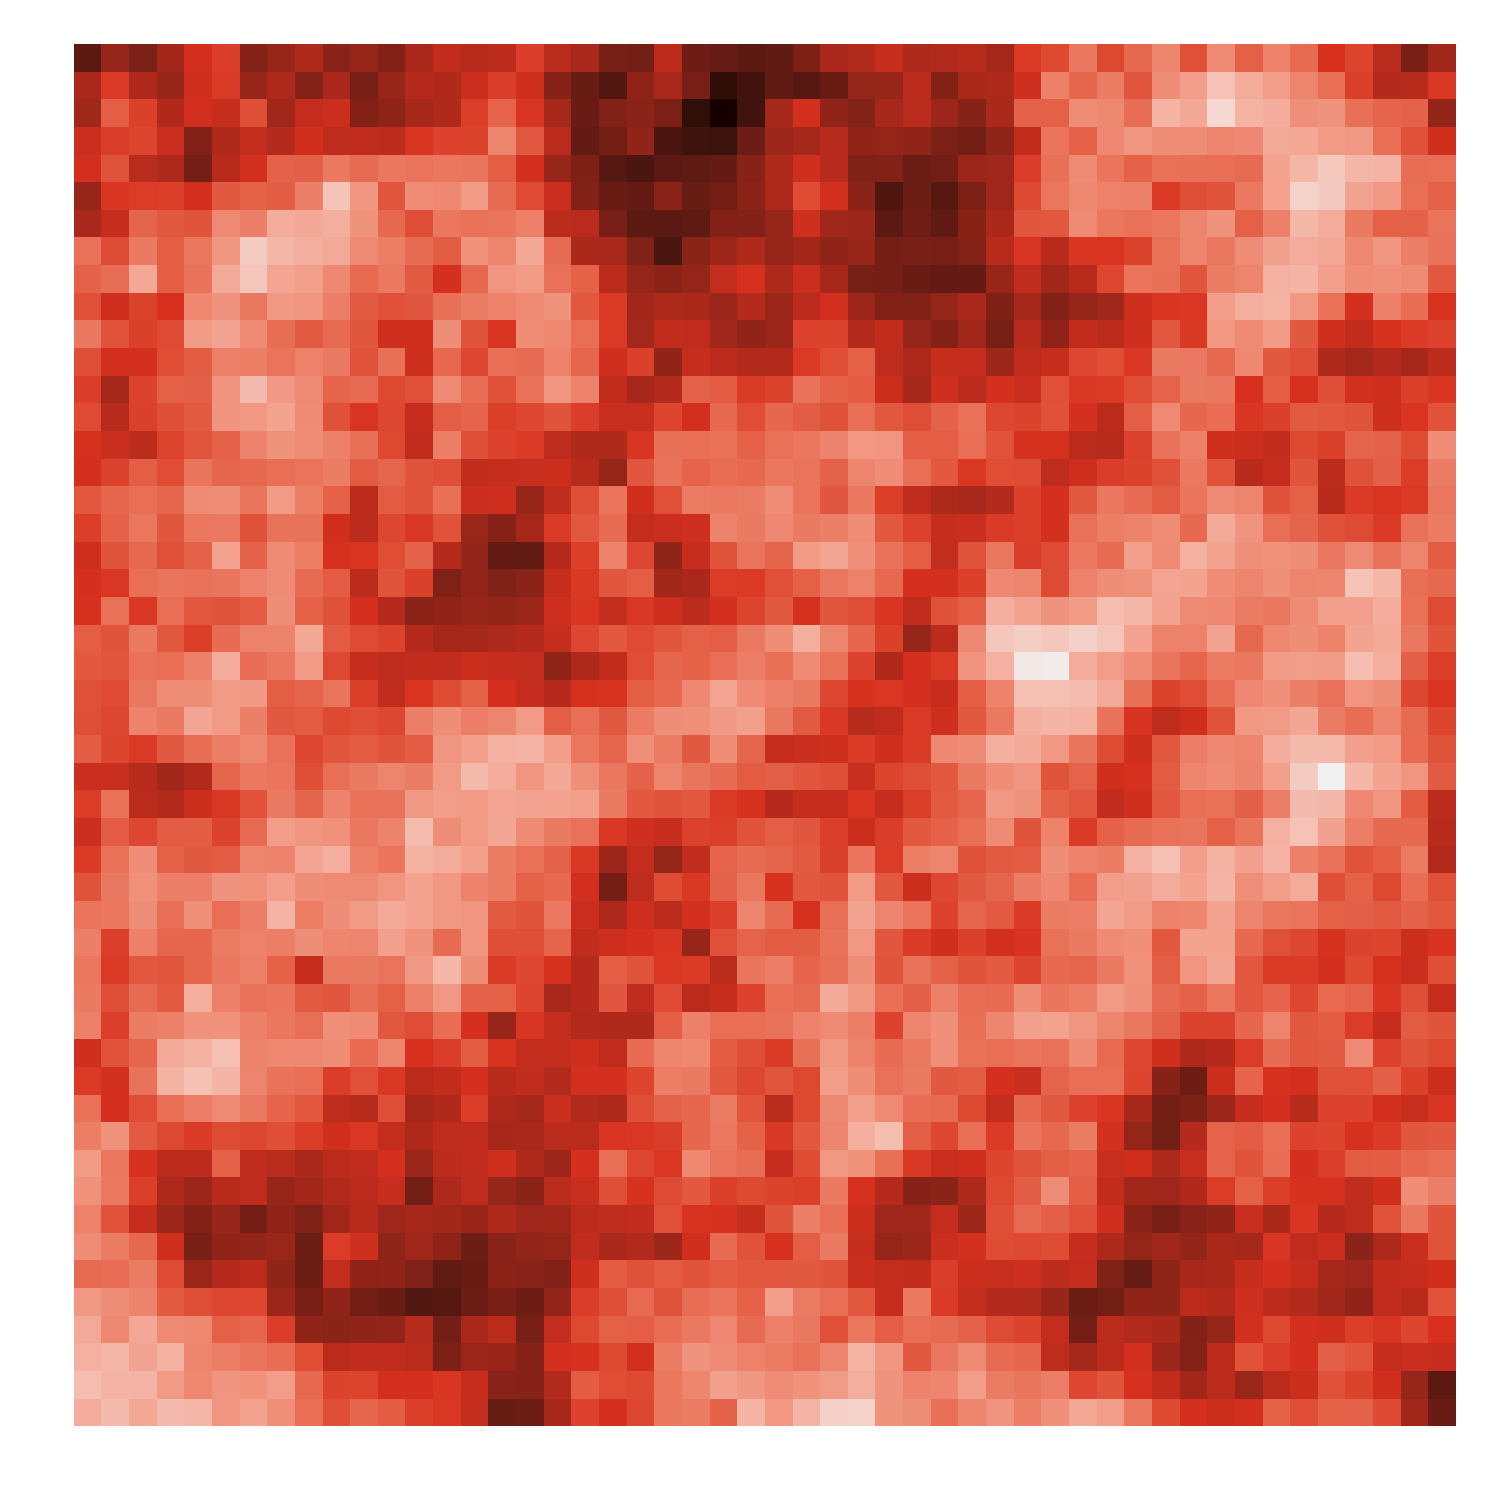
\includegraphics[width=\linewidth]{figures/p_realistic1}\\
 		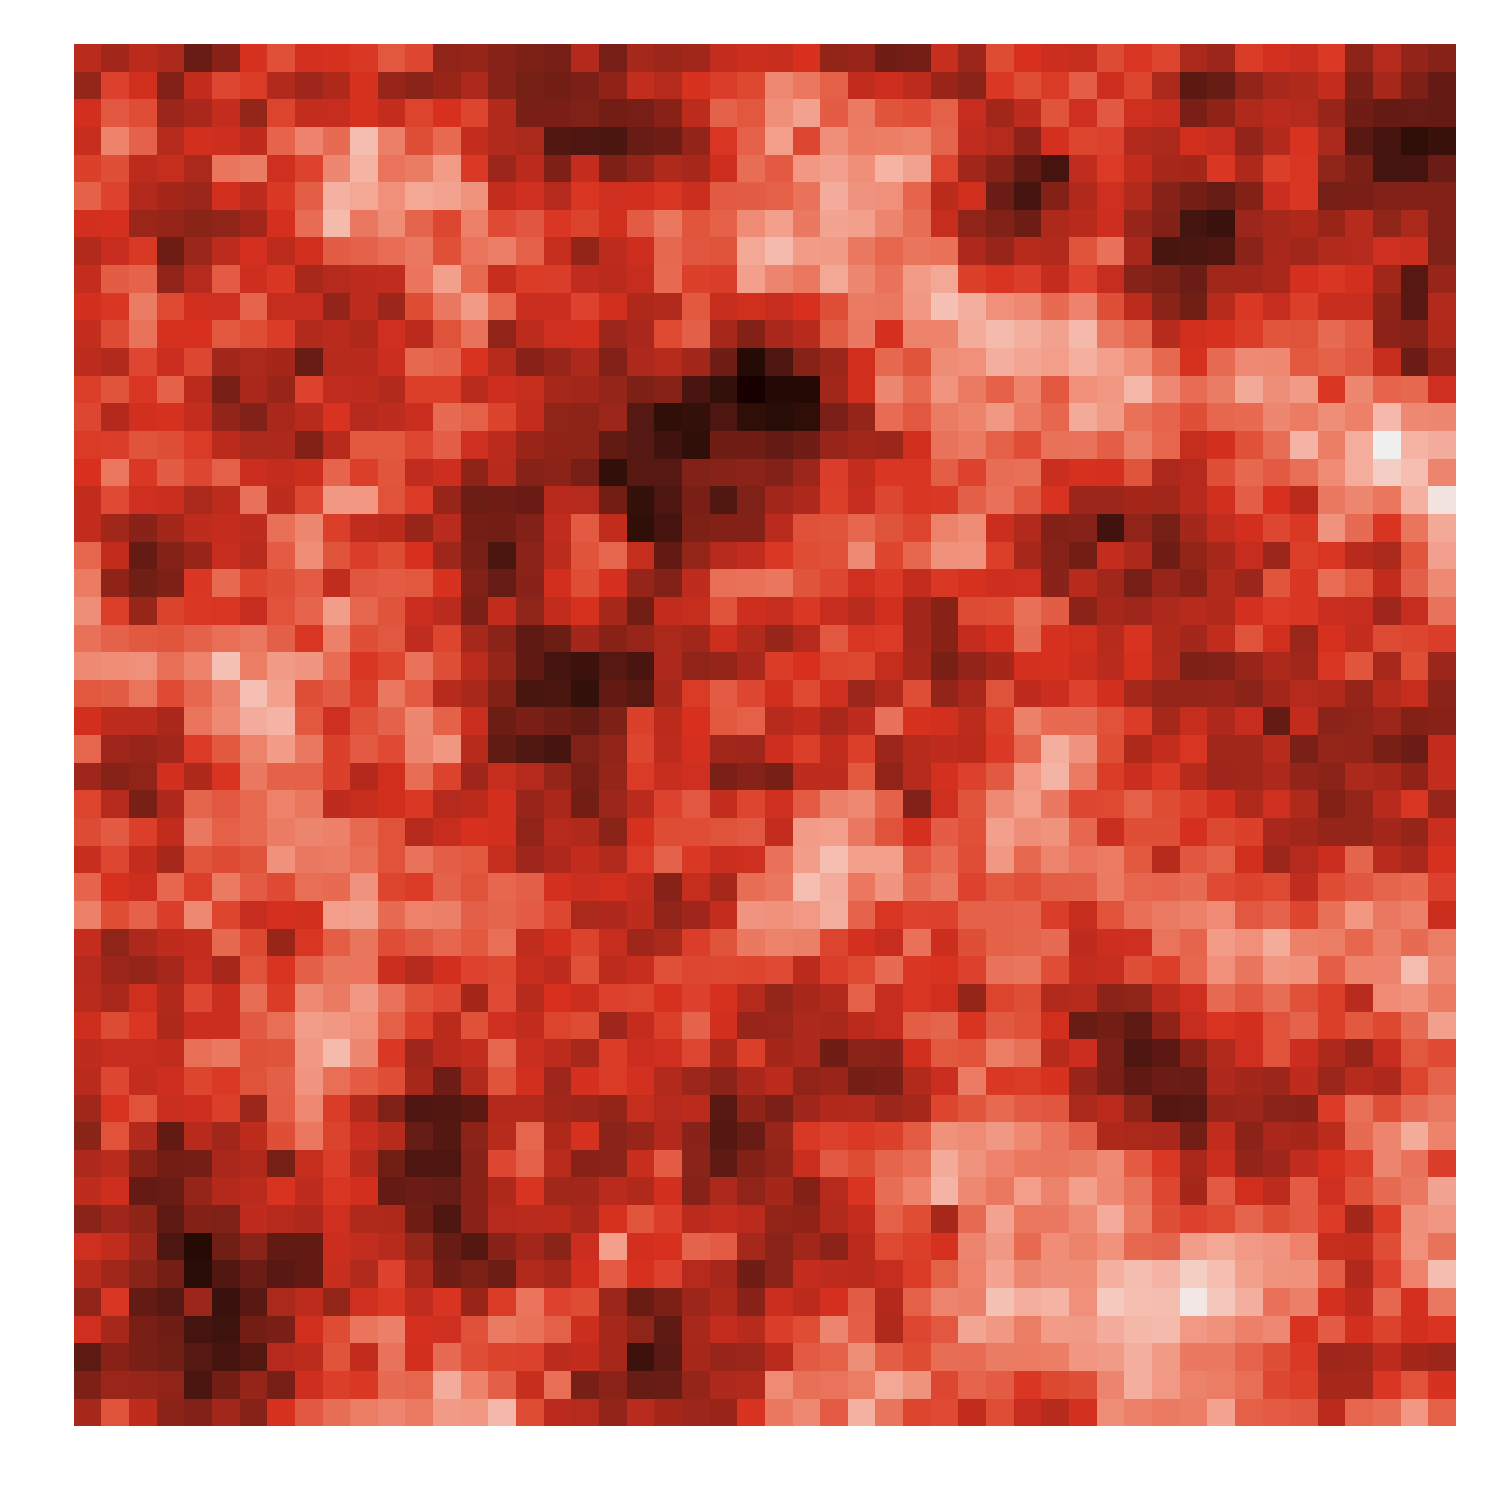
\includegraphics[width=\linewidth]{figures/p_realistic2}\\
 		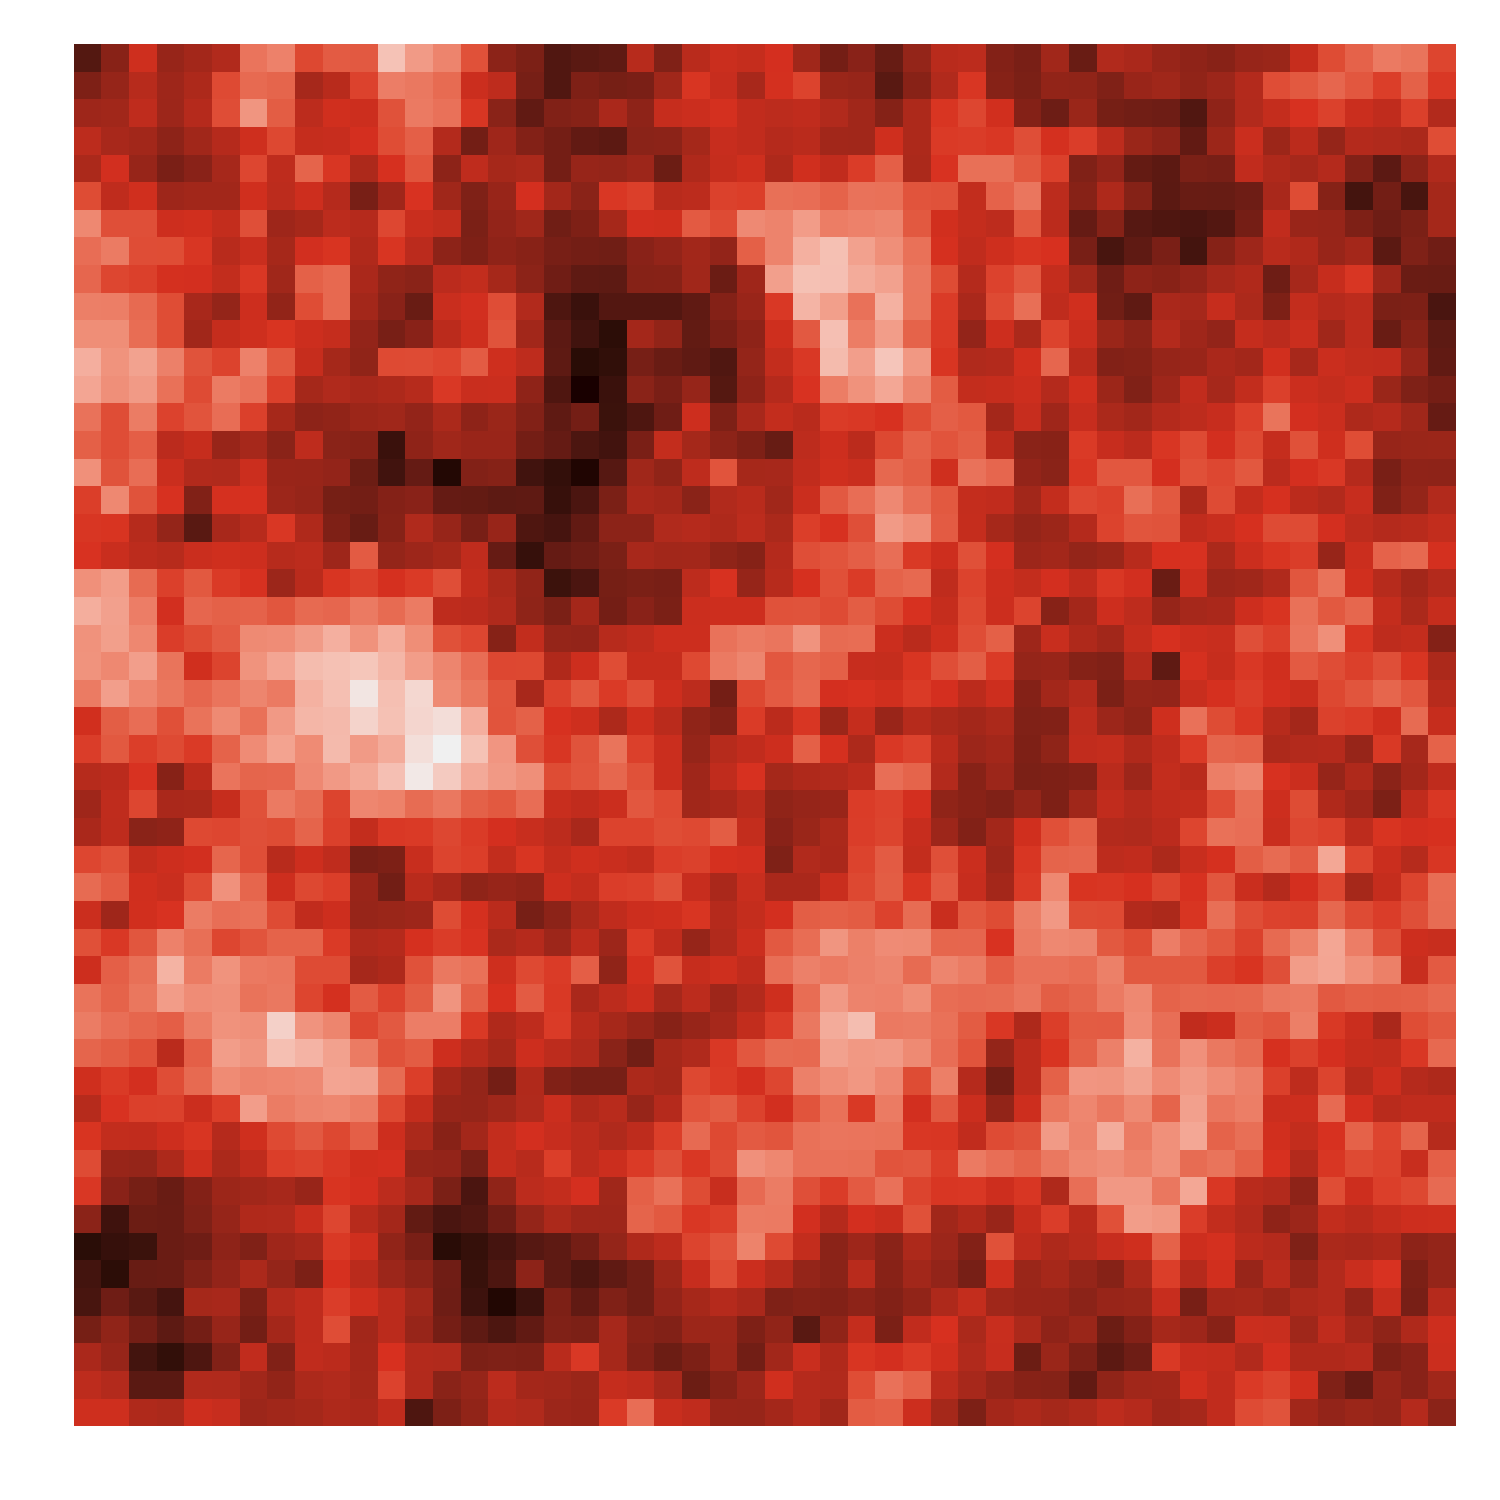
\includegraphics[width=\linewidth]{figures/p_realistic3}\\
 		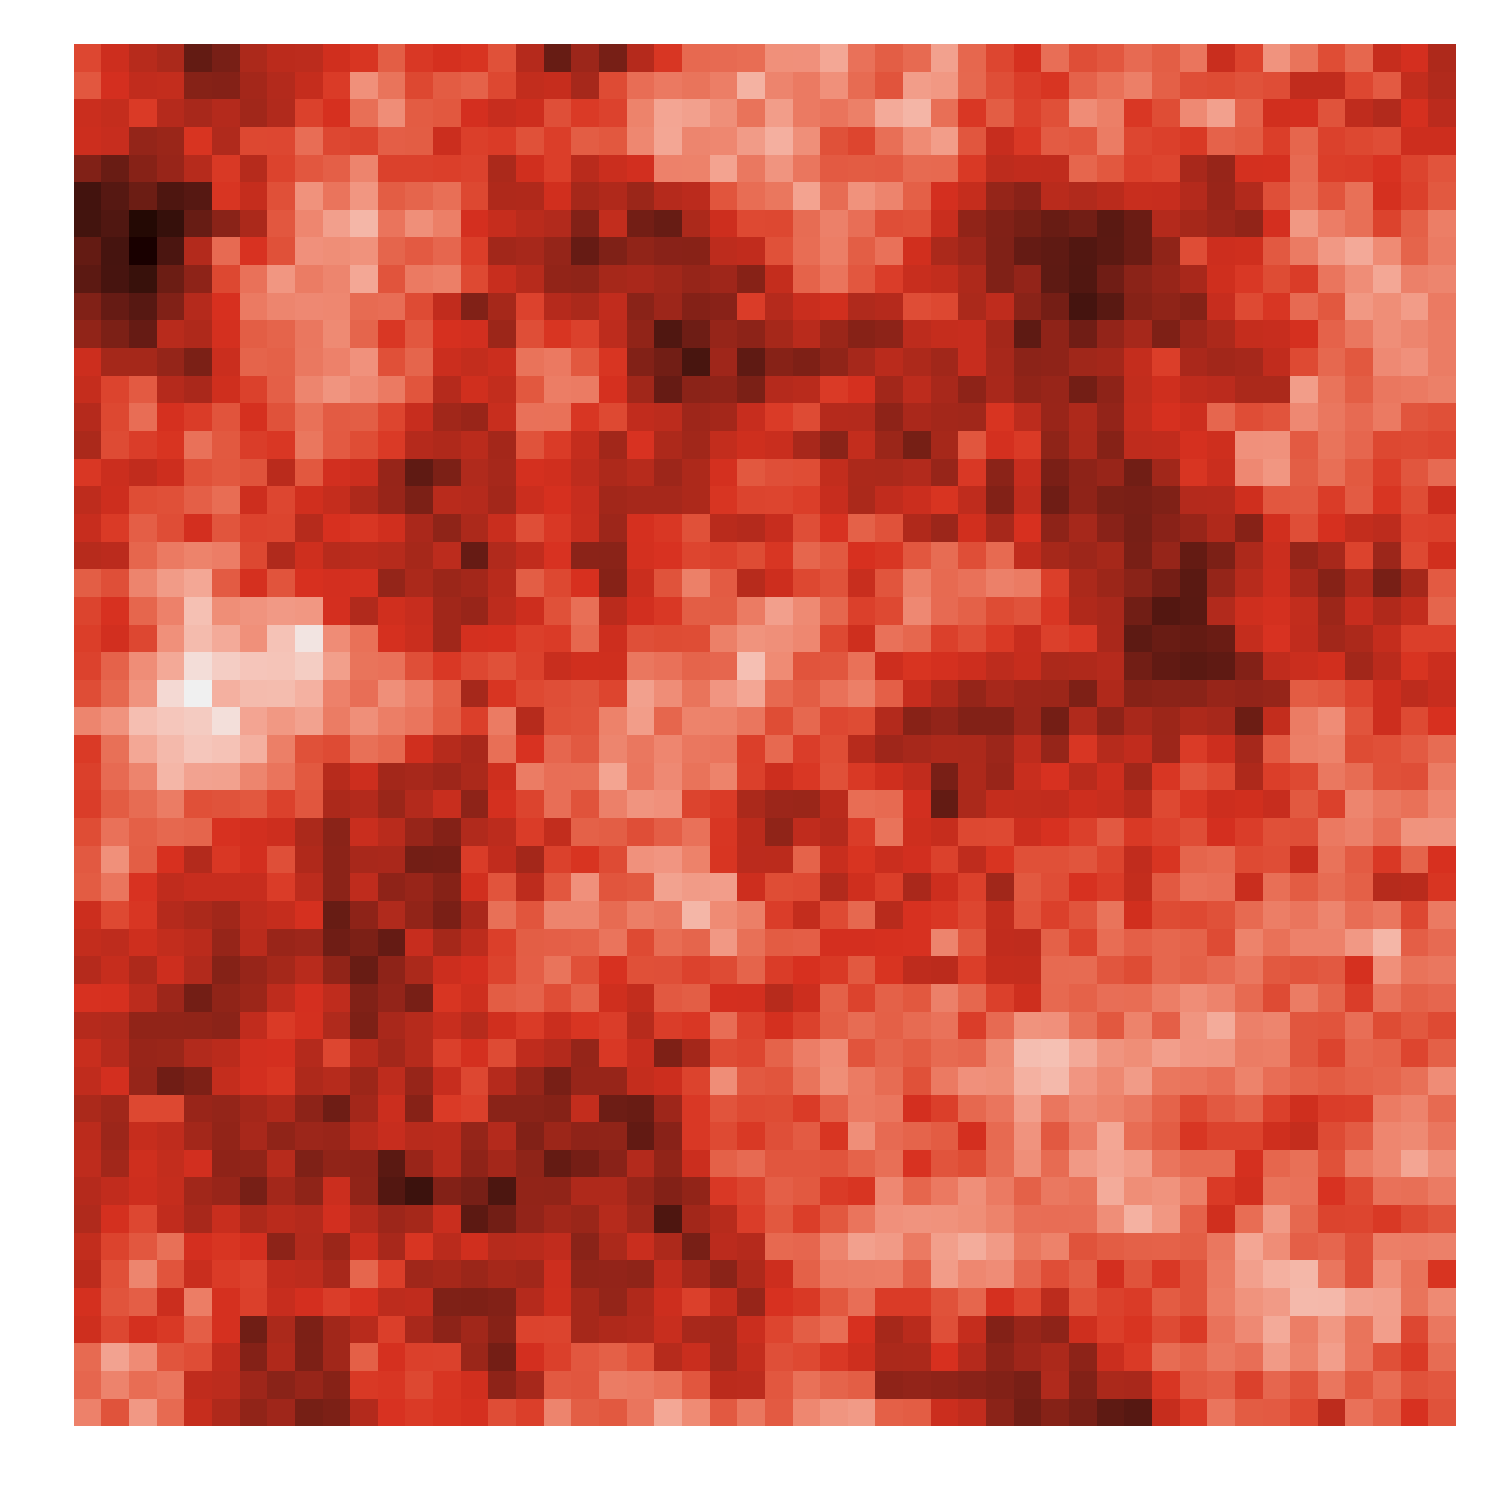
\includegraphics[width=\linewidth]{figures/p_realistic4}\\
 		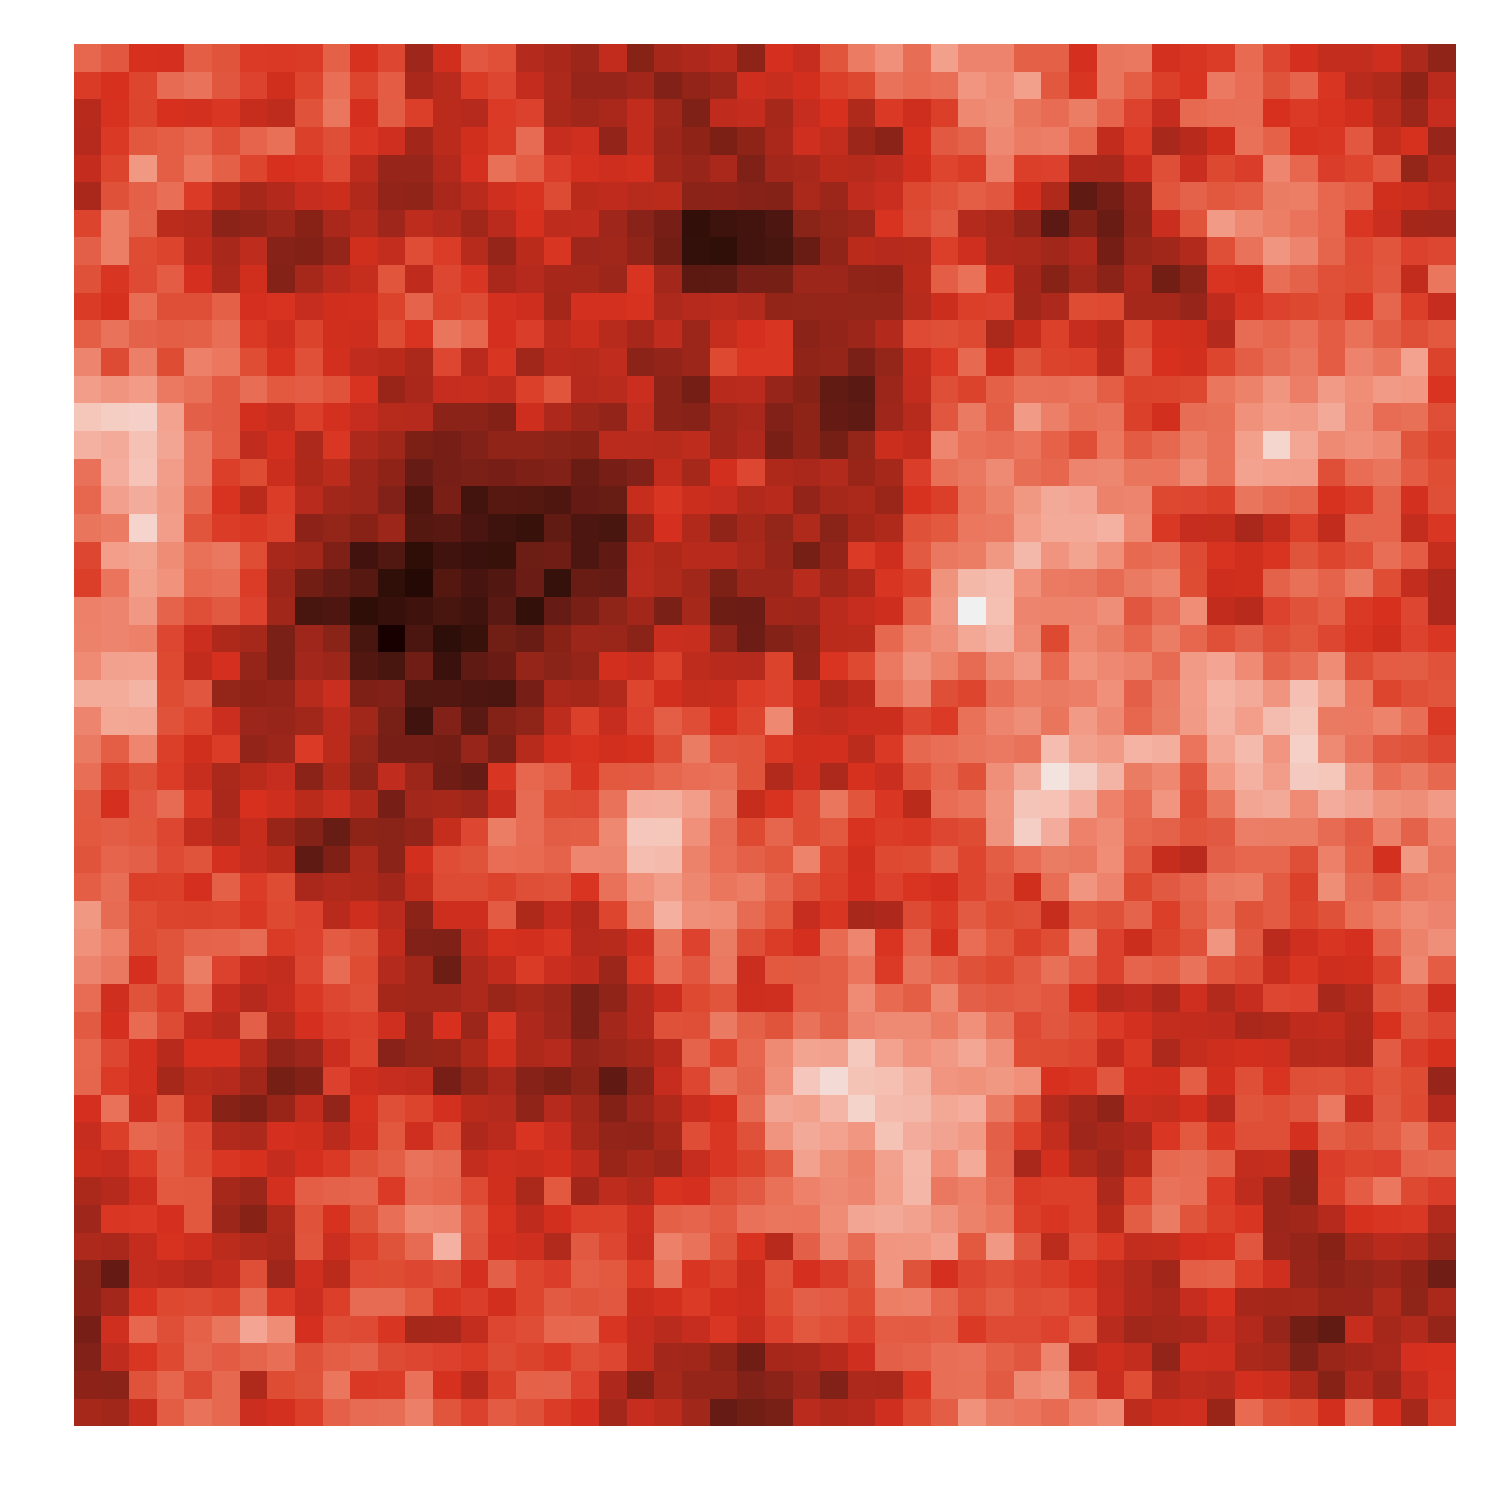
\includegraphics[width=\linewidth]{figures/p_realistic5}\\
 		%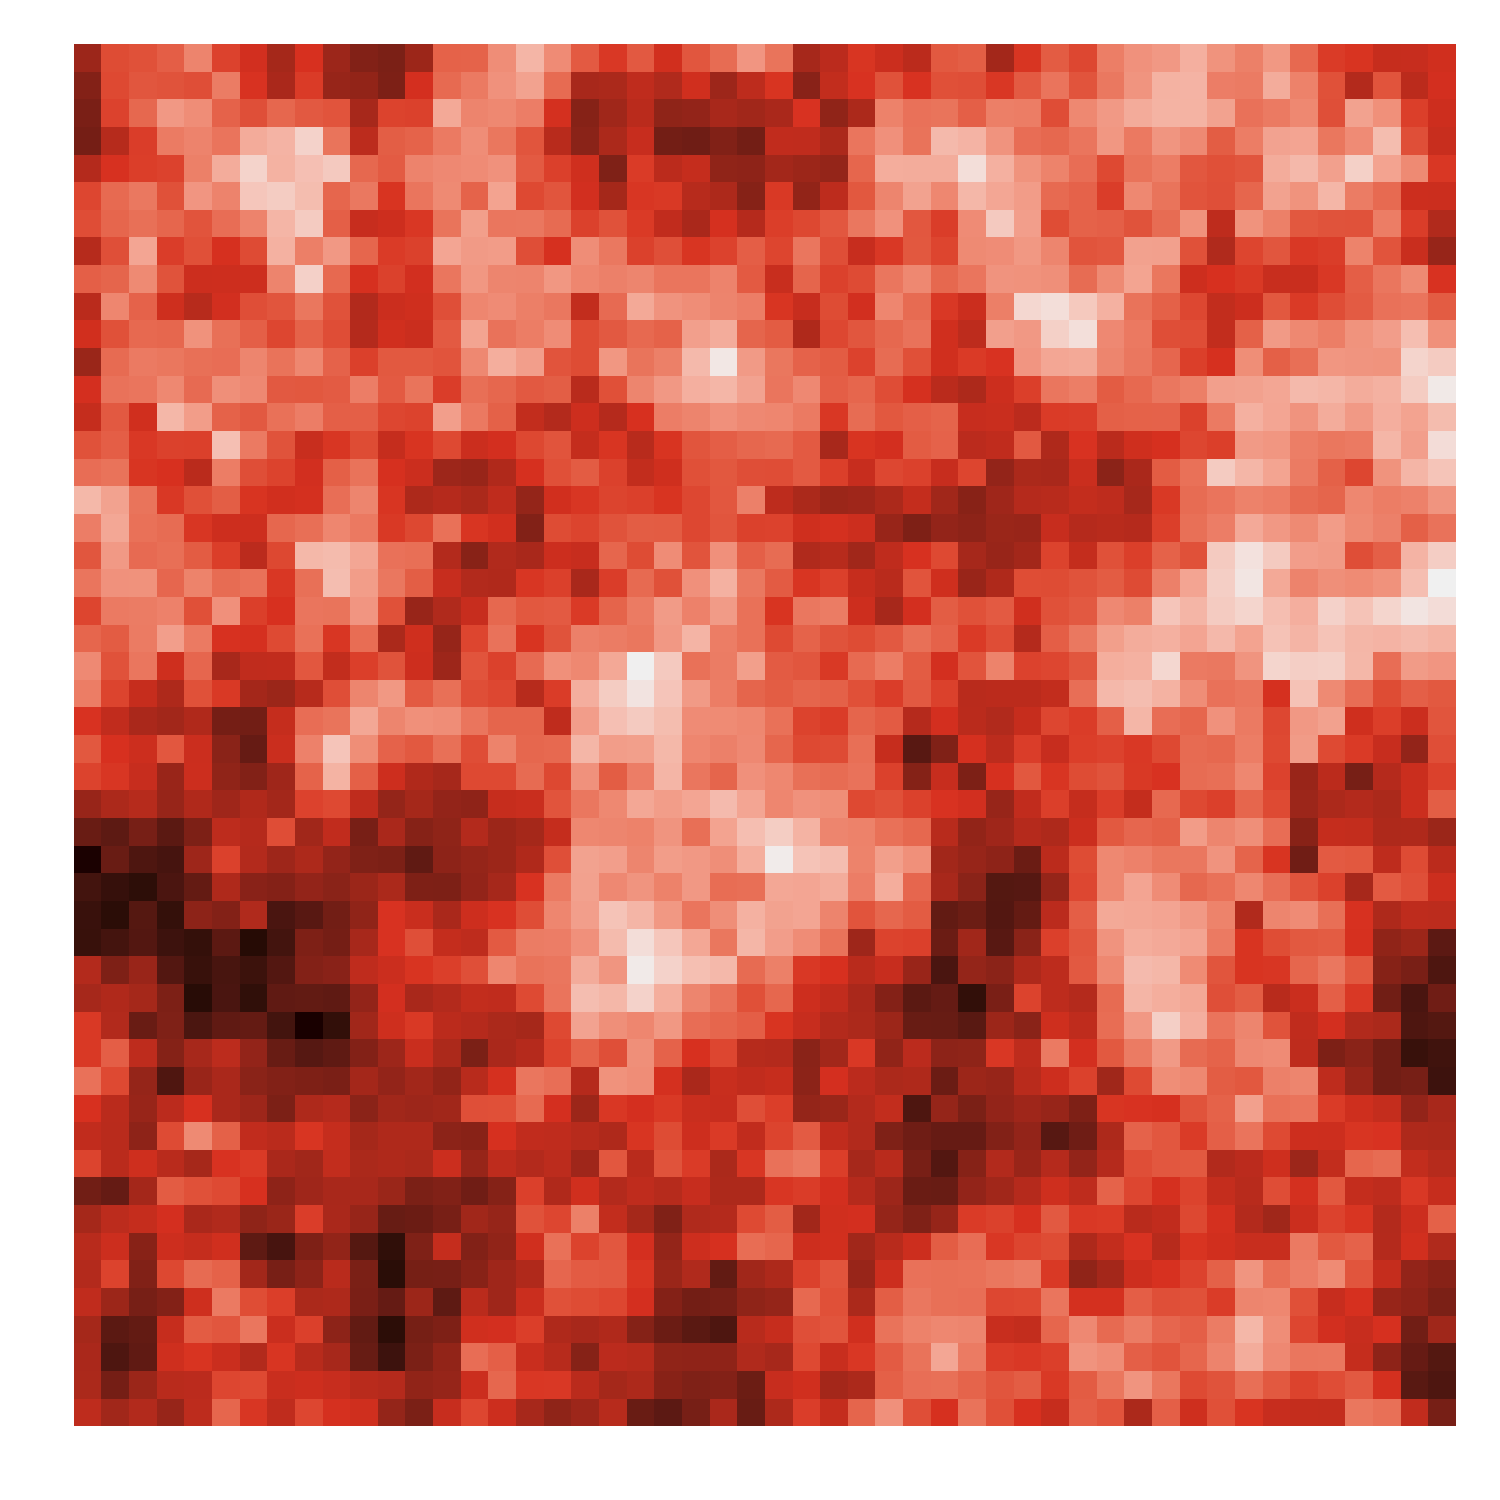
\includegraphics[width=\linewidth]{figures/p_realistic6}\\
 		%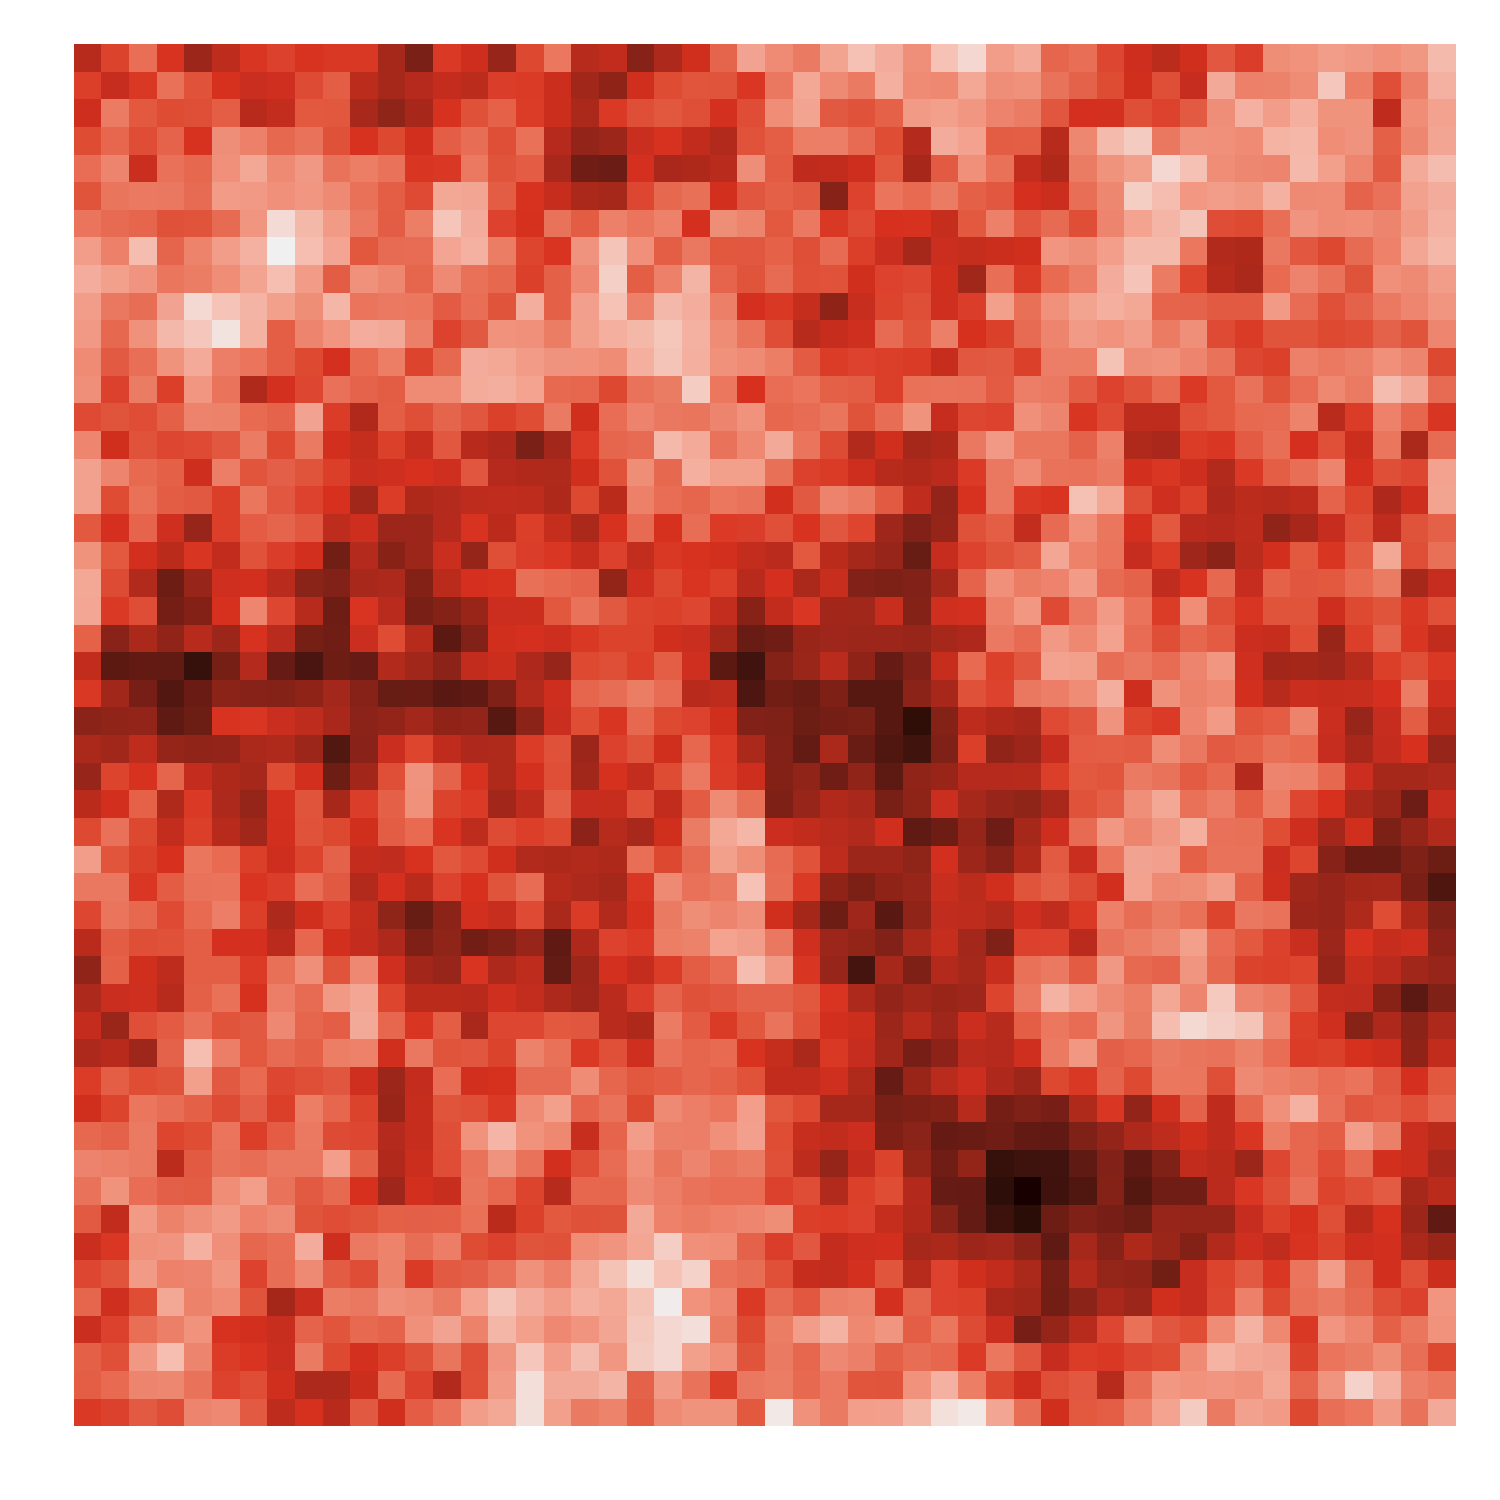
\includegraphics[width=\linewidth]{figures/p_realistic7}\\
 		%\caption{First}
 	\end{subfigure}
 	\begin{subfigure}{0.3\textwidth}
 		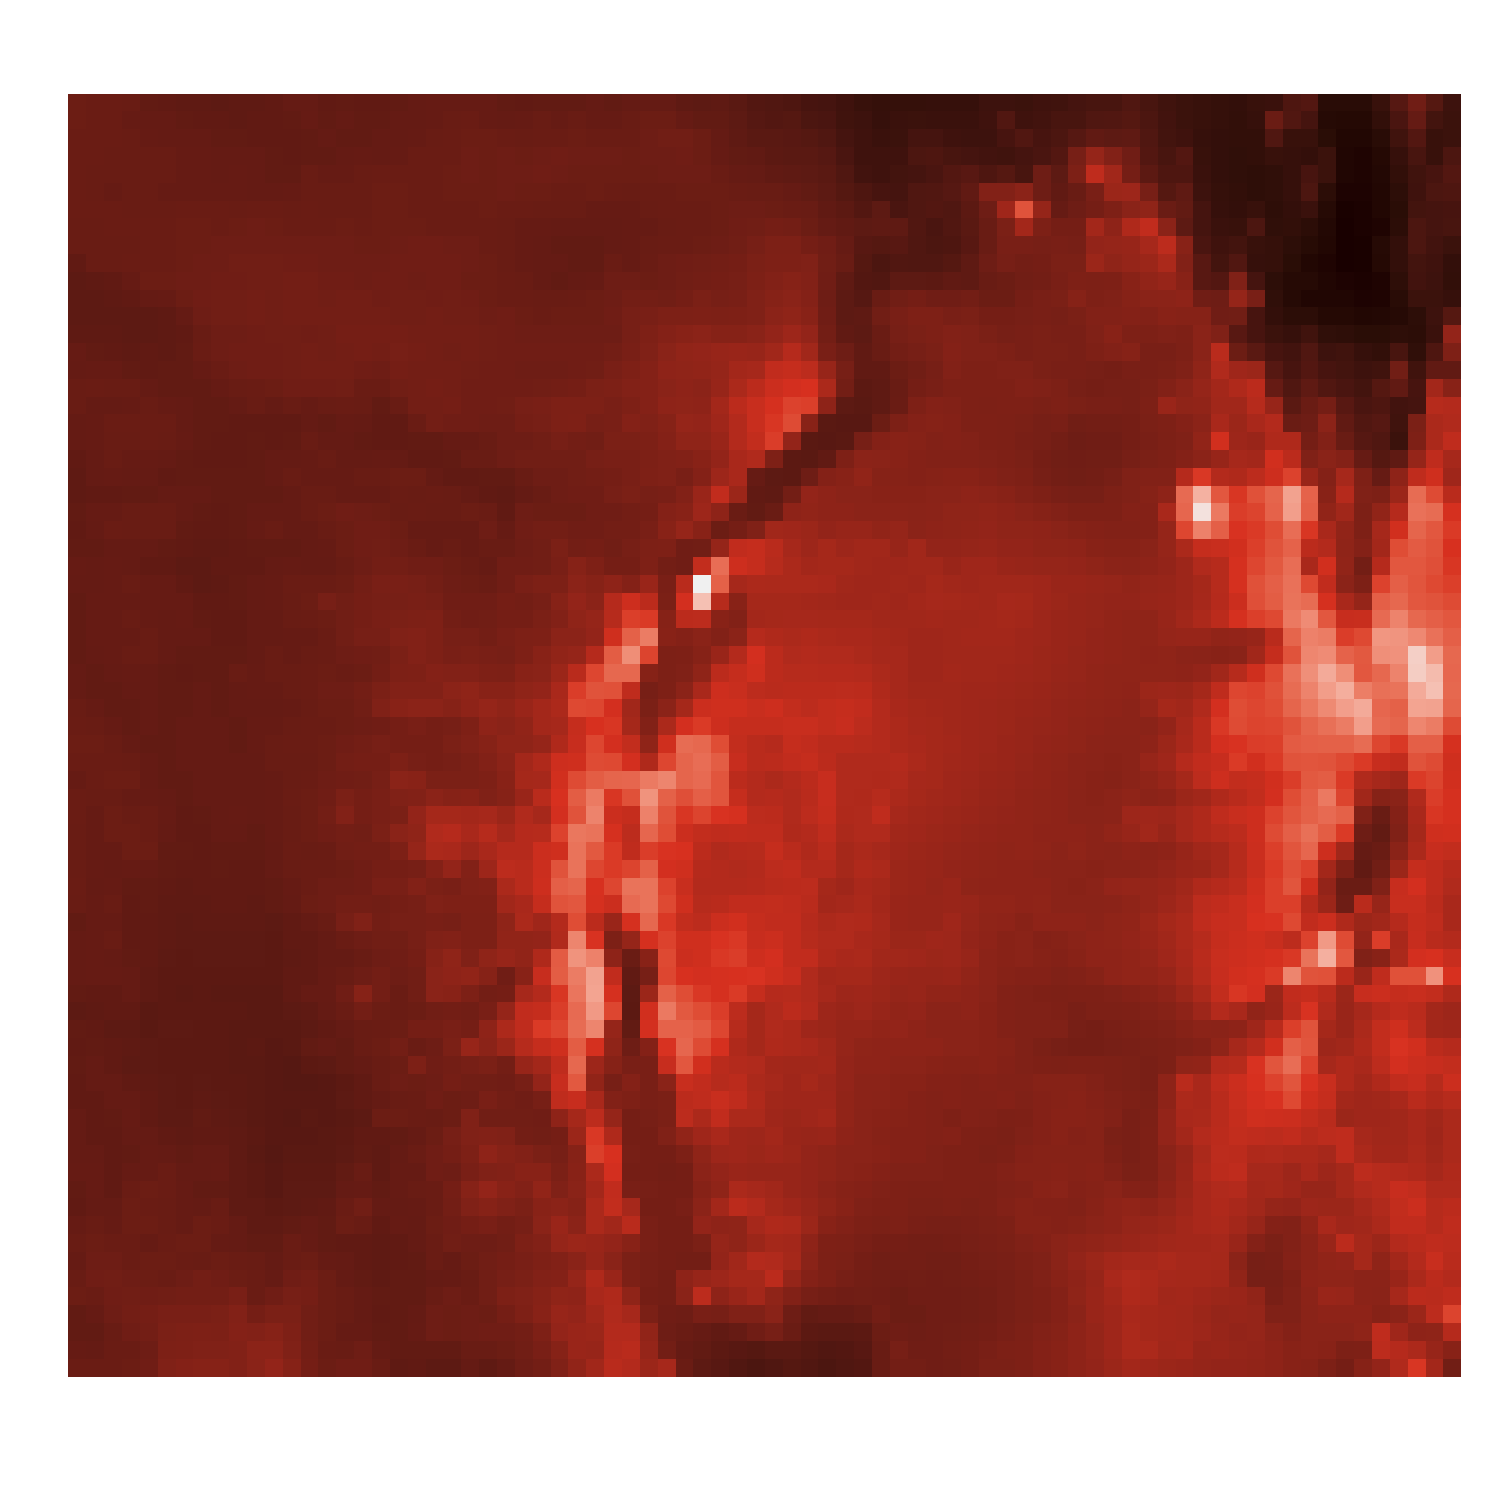
\includegraphics[width=\linewidth]{figures/p_real1}\\
 		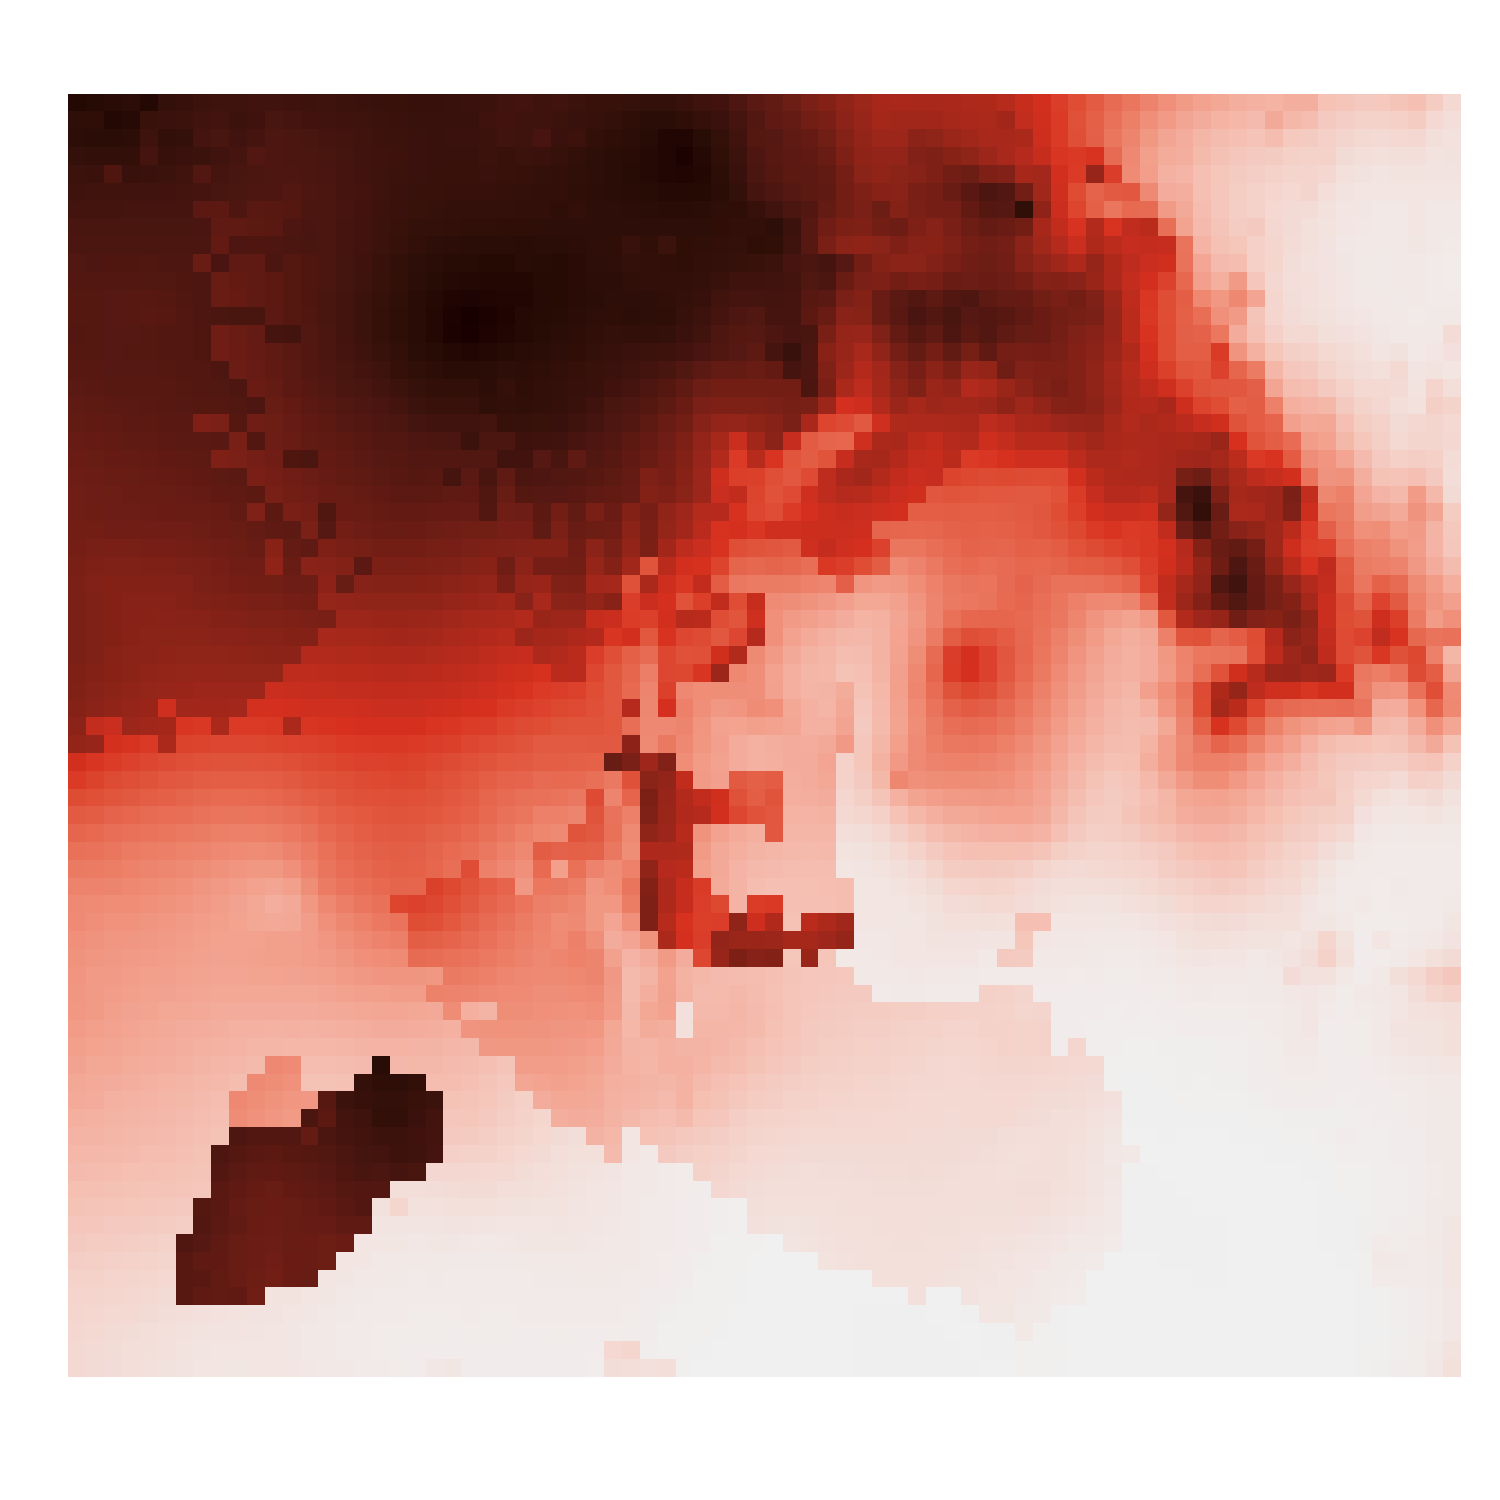
\includegraphics[width=\linewidth]{figures/p_real2}\\
 		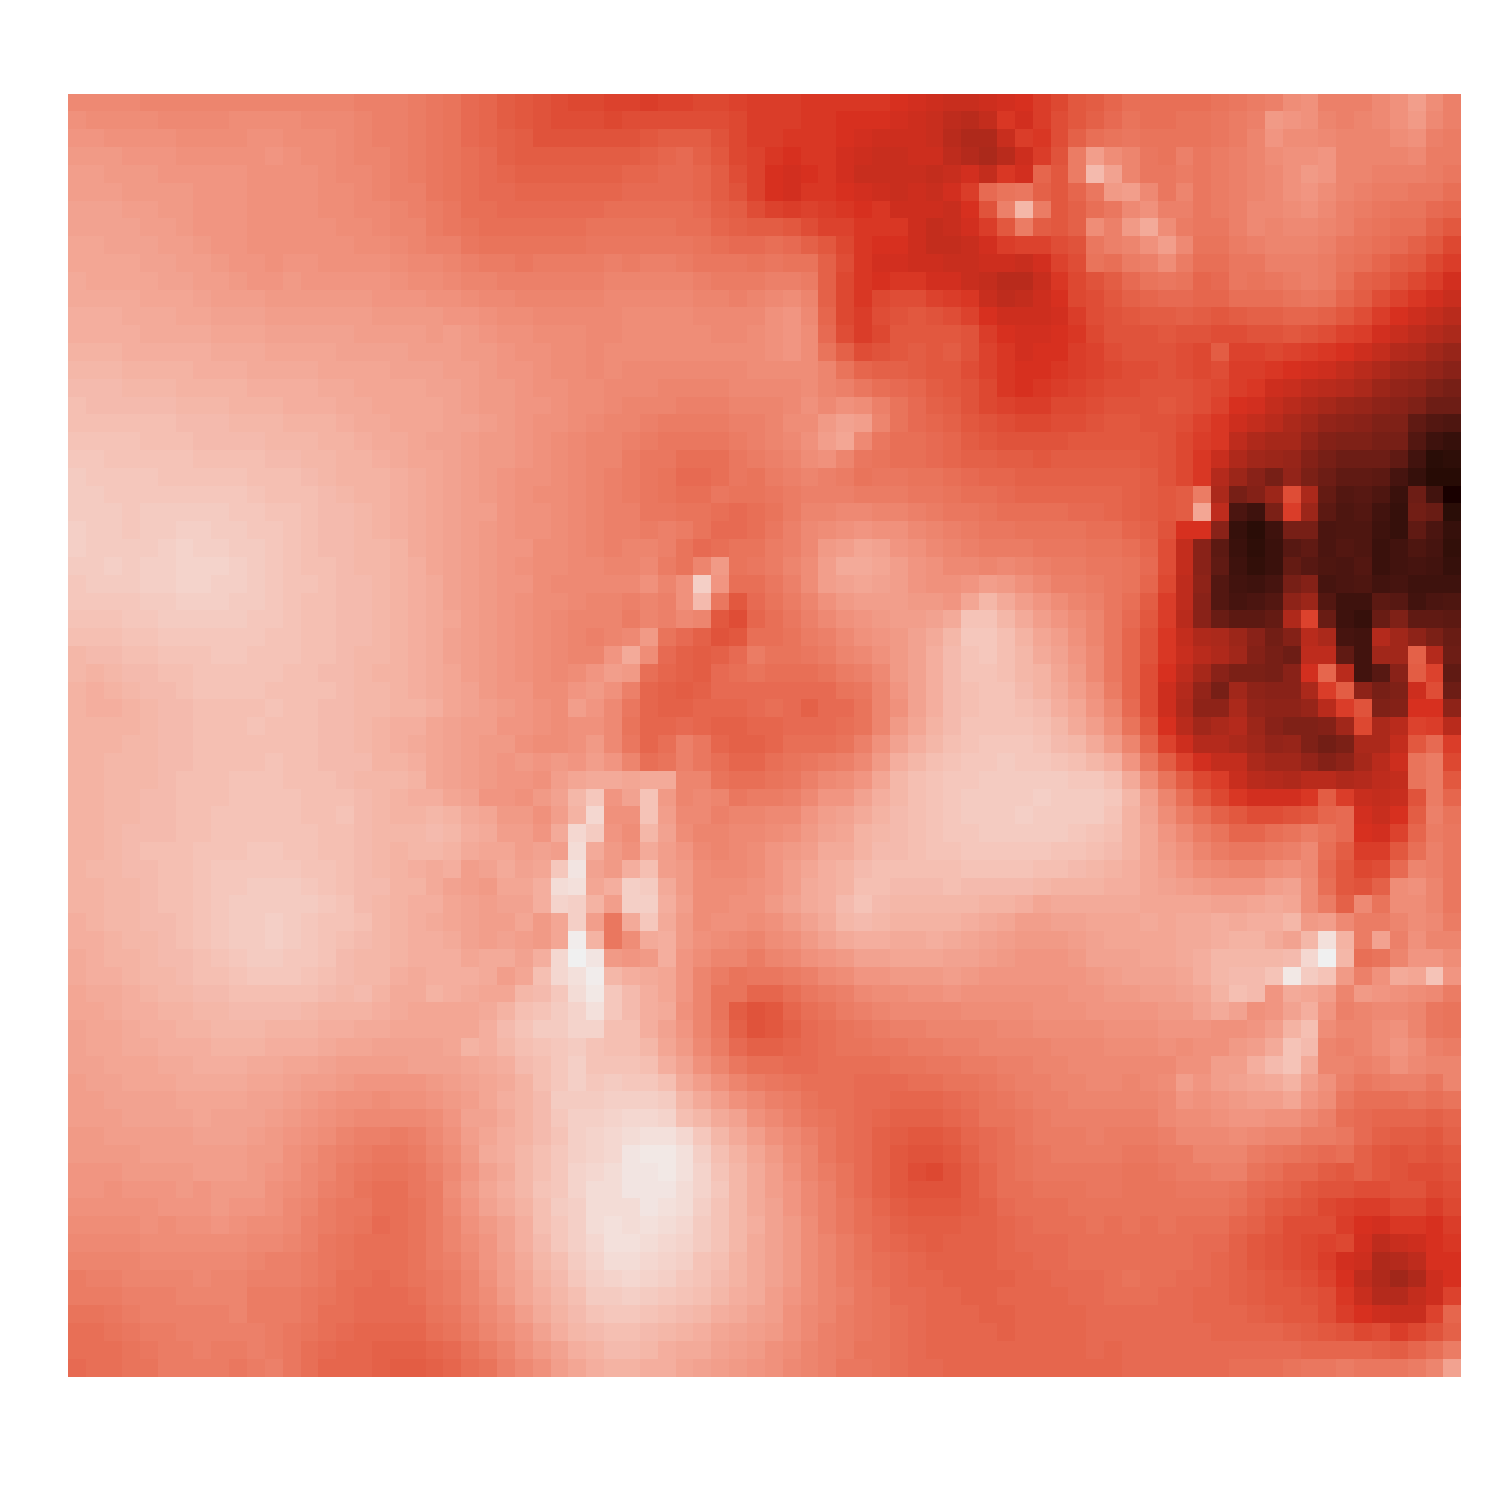
\includegraphics[width=\linewidth]{figures/p_real3}\\
 		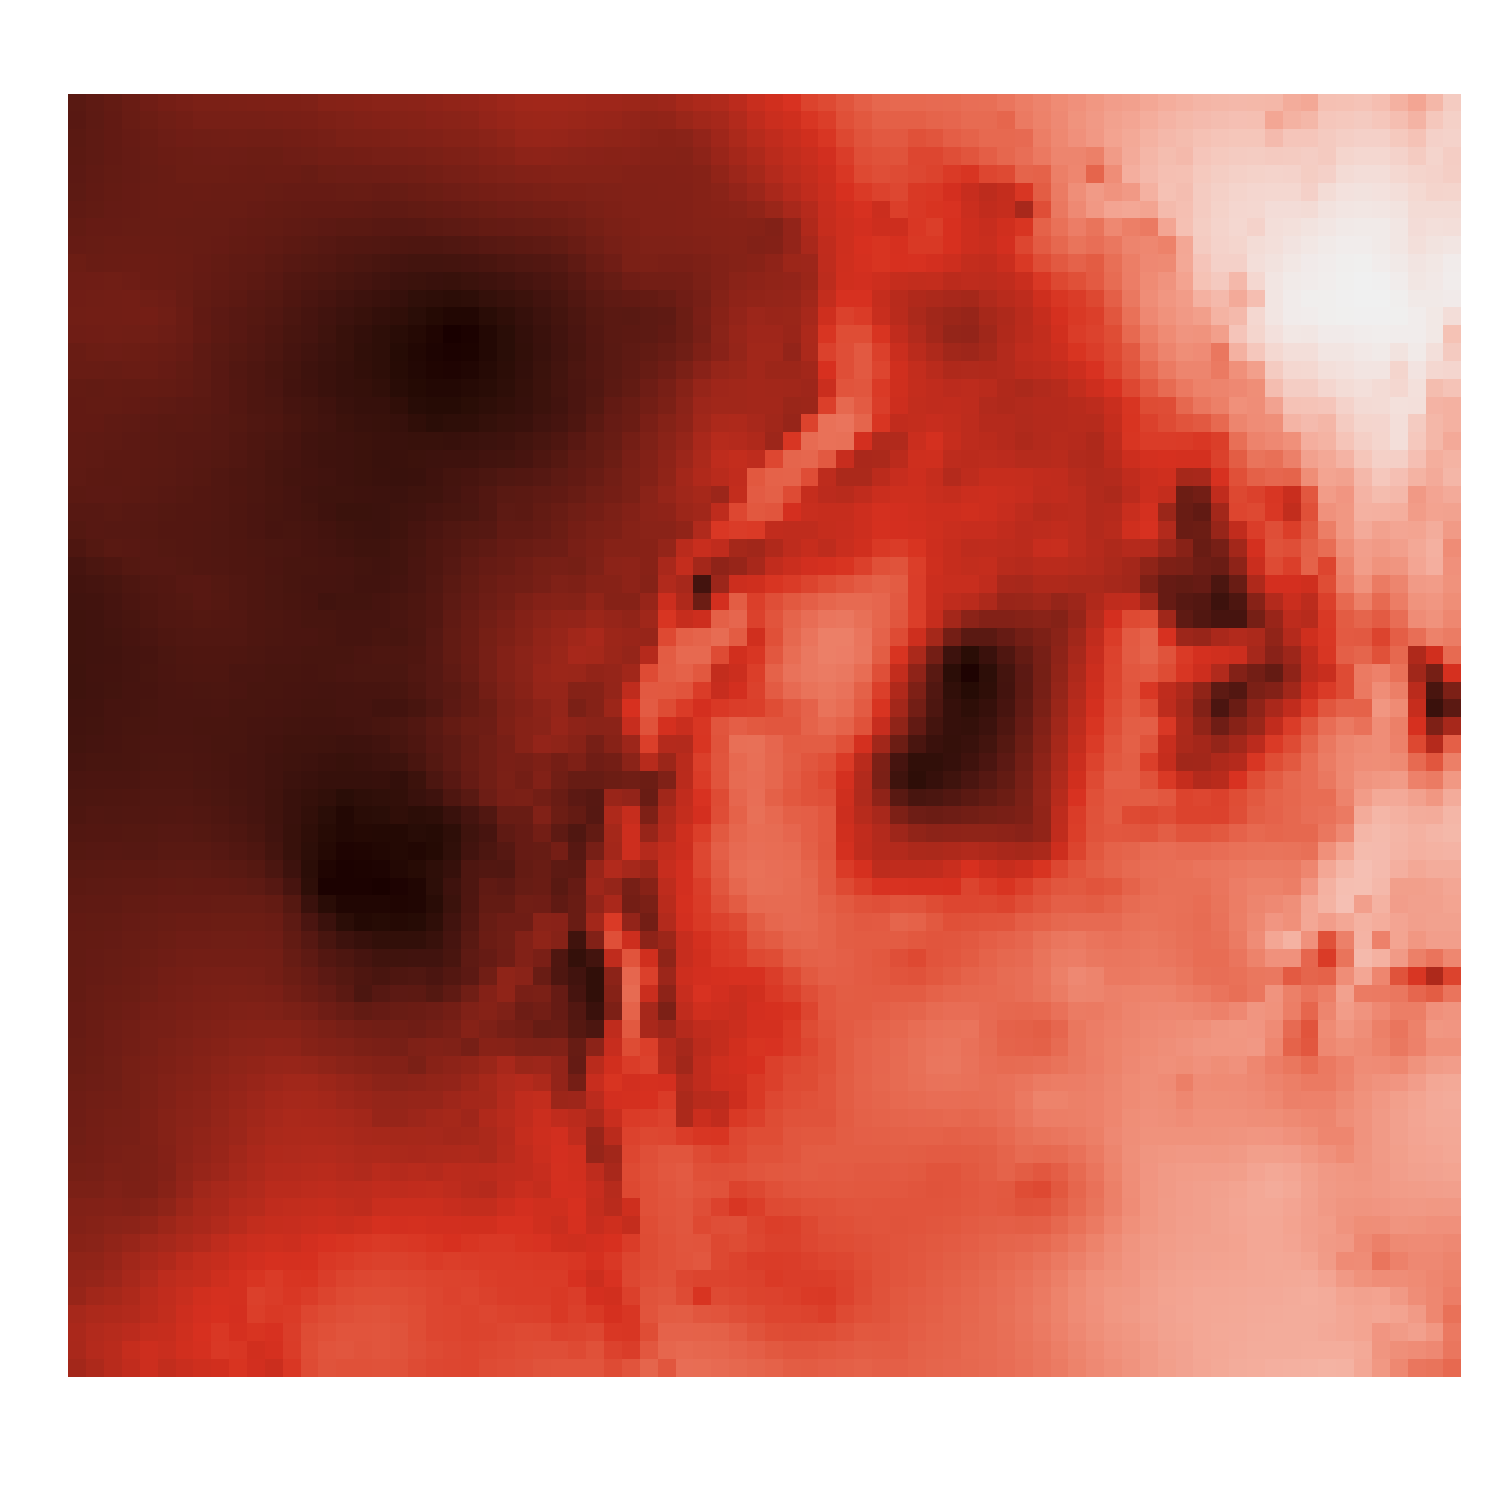
\includegraphics[width=\linewidth]{figures/p_real4}\\
 		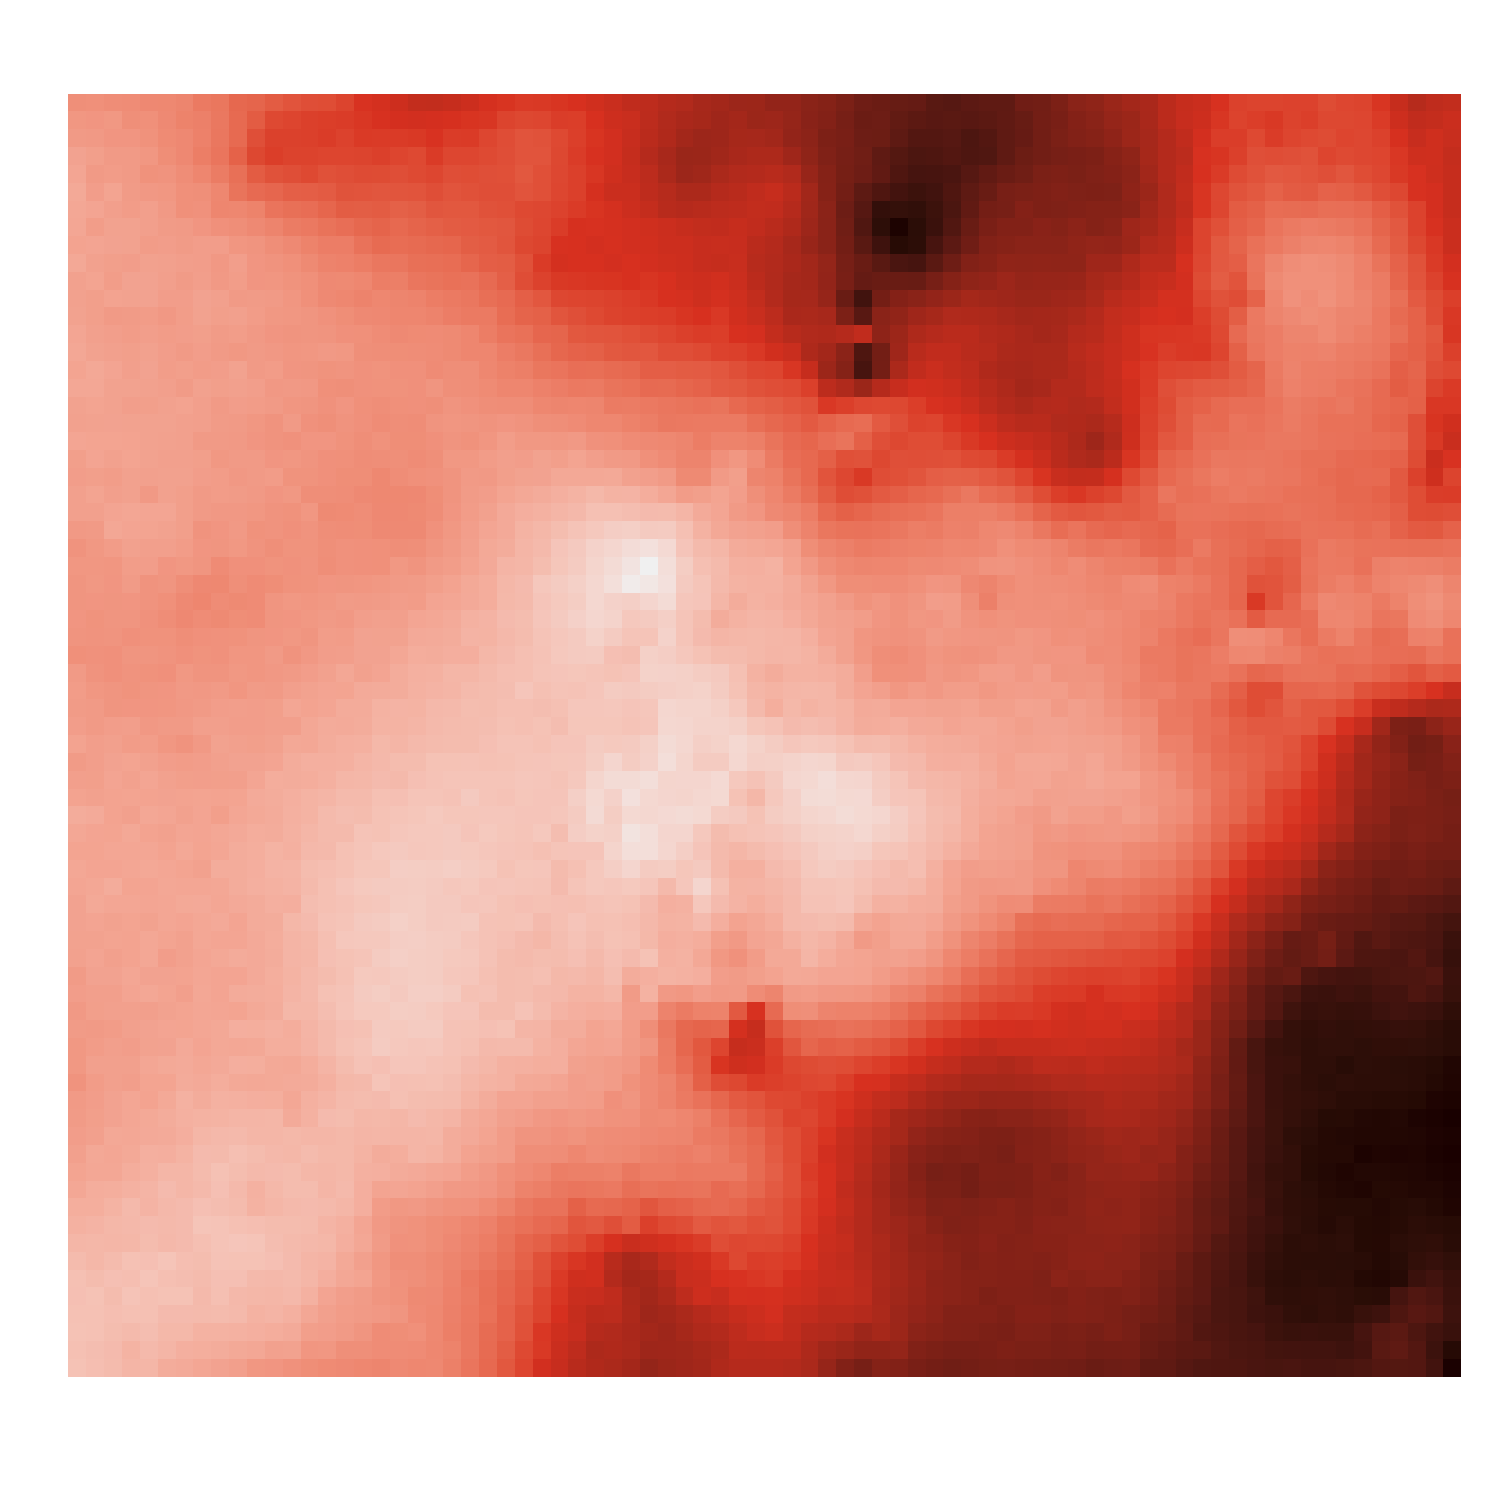
\includegraphics[width=\linewidth]{figures/p_real5}\\
 		%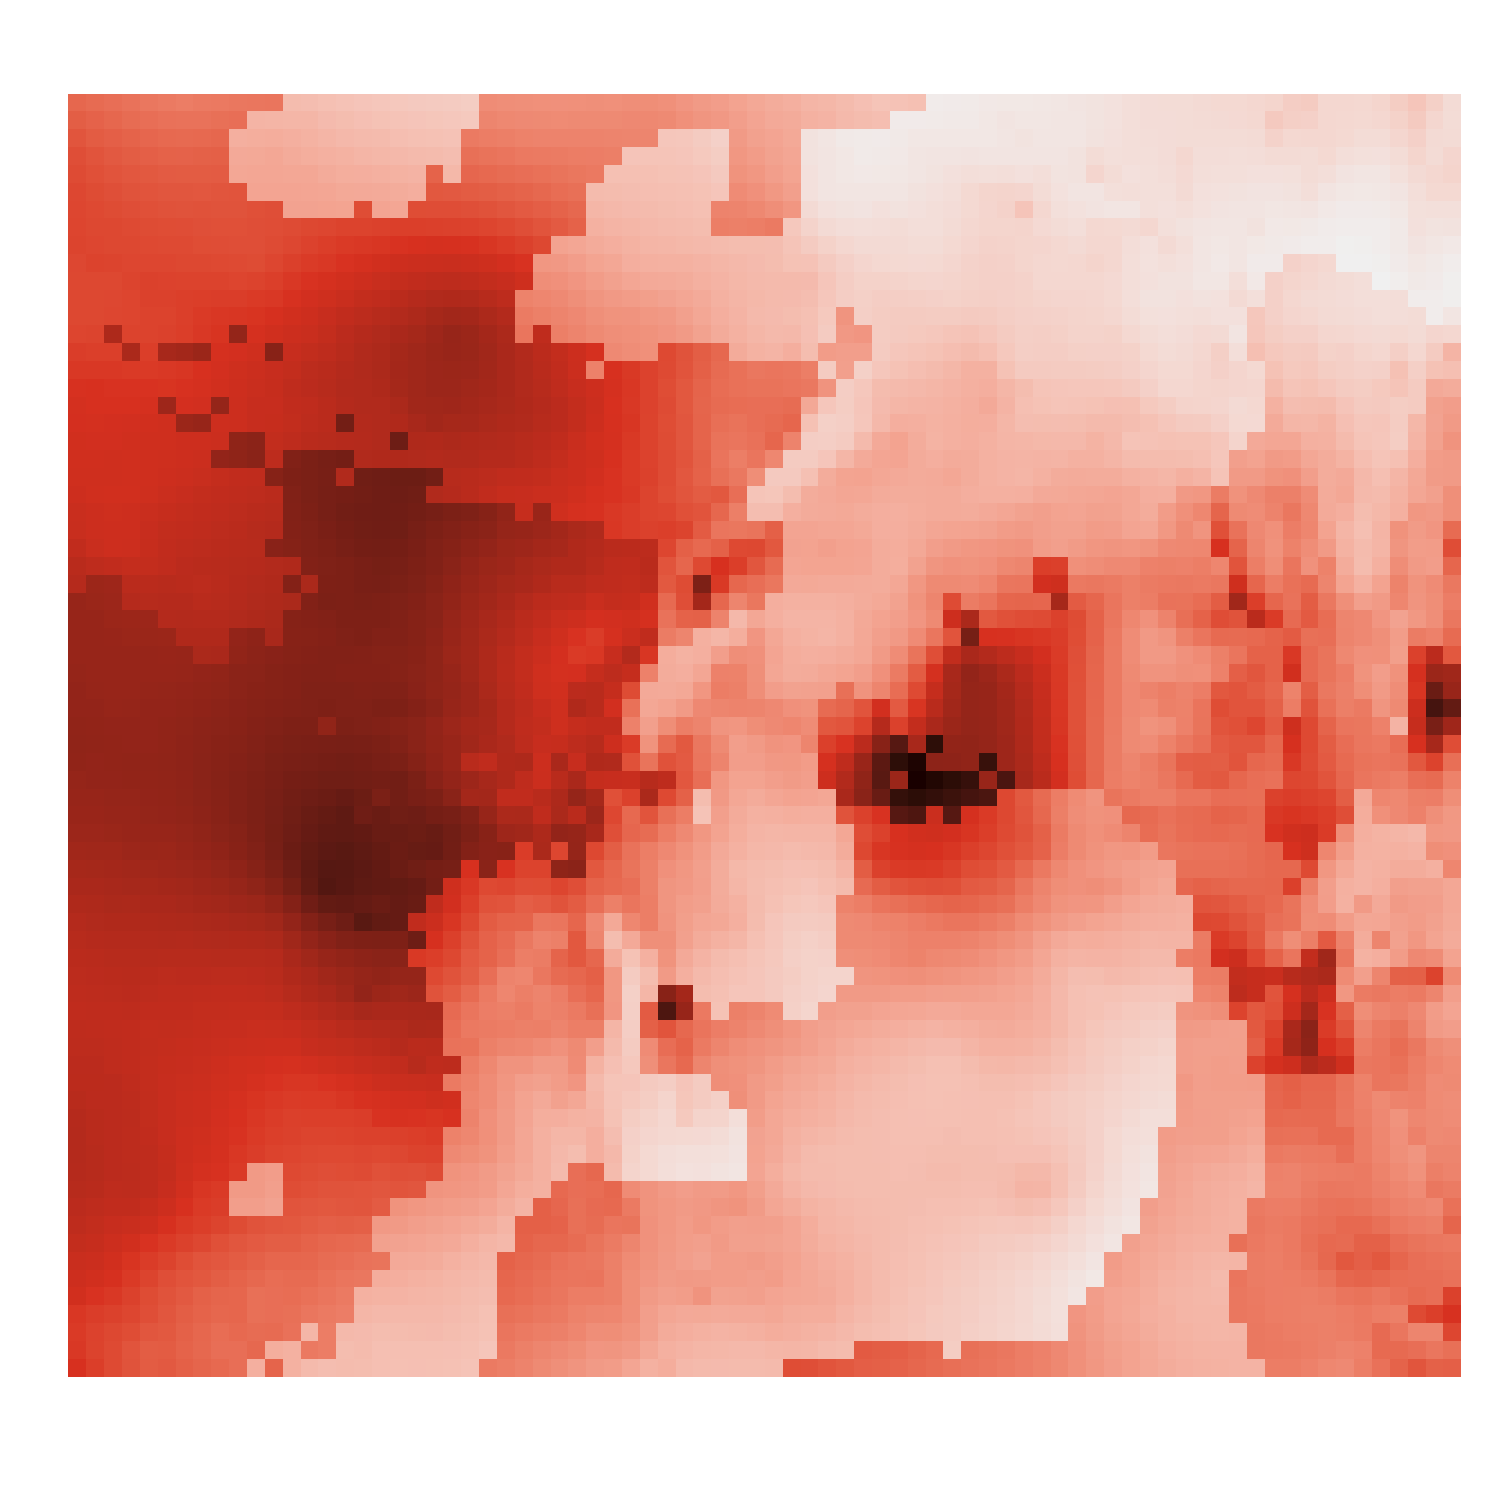
\includegraphics[width=\linewidth]{figures/p_real6}\\
 		%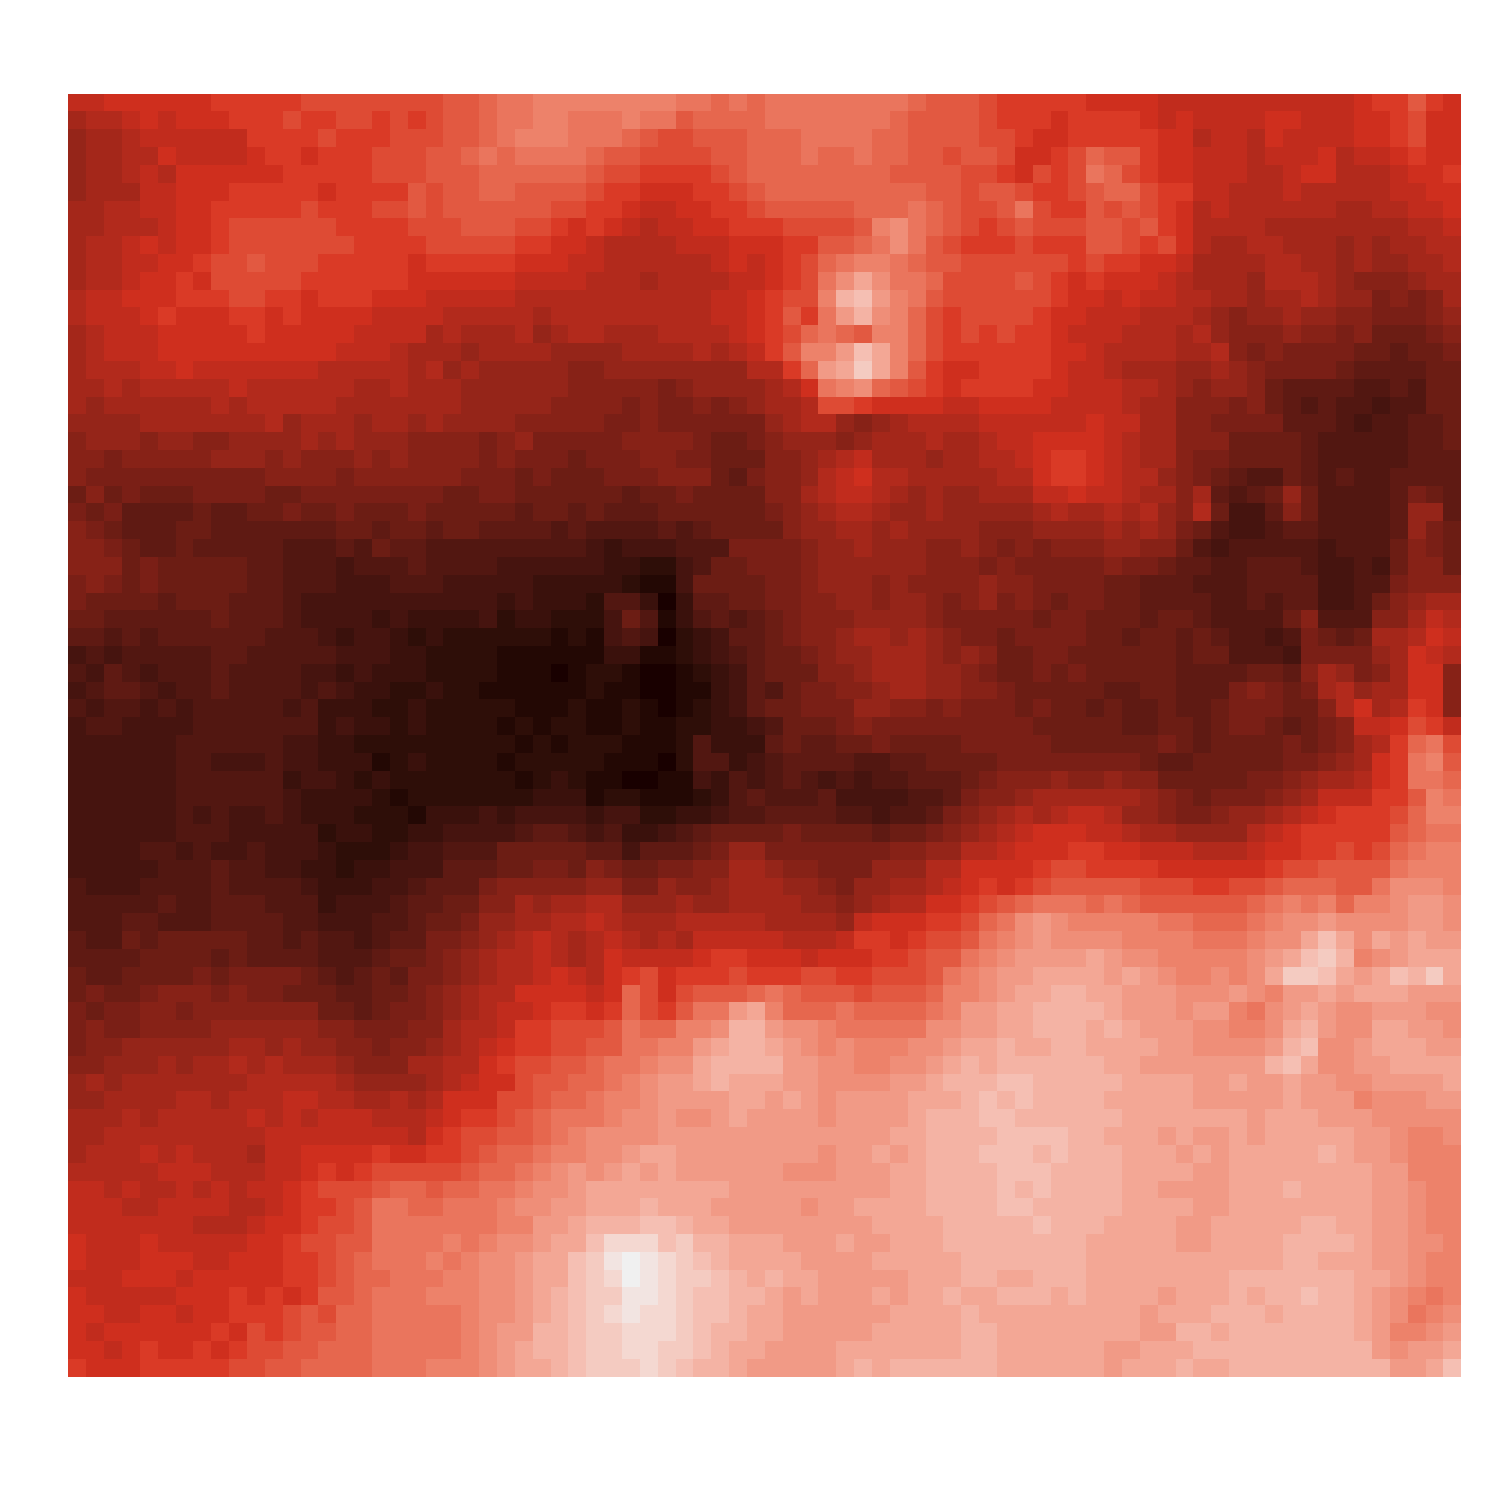
\includegraphics[width=\linewidth]{figures/p_real7}\\
 		%\caption{First}
 	\end{subfigure}
 	\begin{subfigure}{0.08\textwidth}
 		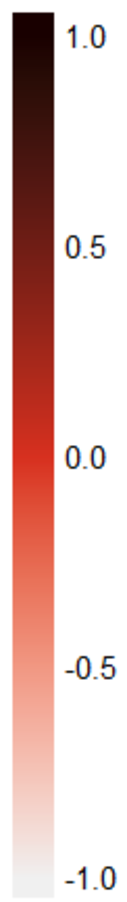
\includegraphics[width=\linewidth]{figures/legend}
 		%\caption{First}
 	\end{subfigure}
 	\put(-430,375){\Large\textsc{smooth}}
 	\put(-290,375){\Large\textsc{realistic}}
 	\put(-135,375){\Large\textsc{real}}
	\put(-495,355){\Large{$x_1$}}
	\put(-495,210){\Large{$x_2$}}
	\put(-495,65){\Large{$x_3$}}
	\put(-495,-80){\Large{$x_4$}}
	\put(-495,-225){\Large{$x_5$}}
\end{figure}

\begin{figure}[t!]
	\begin{subfigure}{0.3\textwidth}
		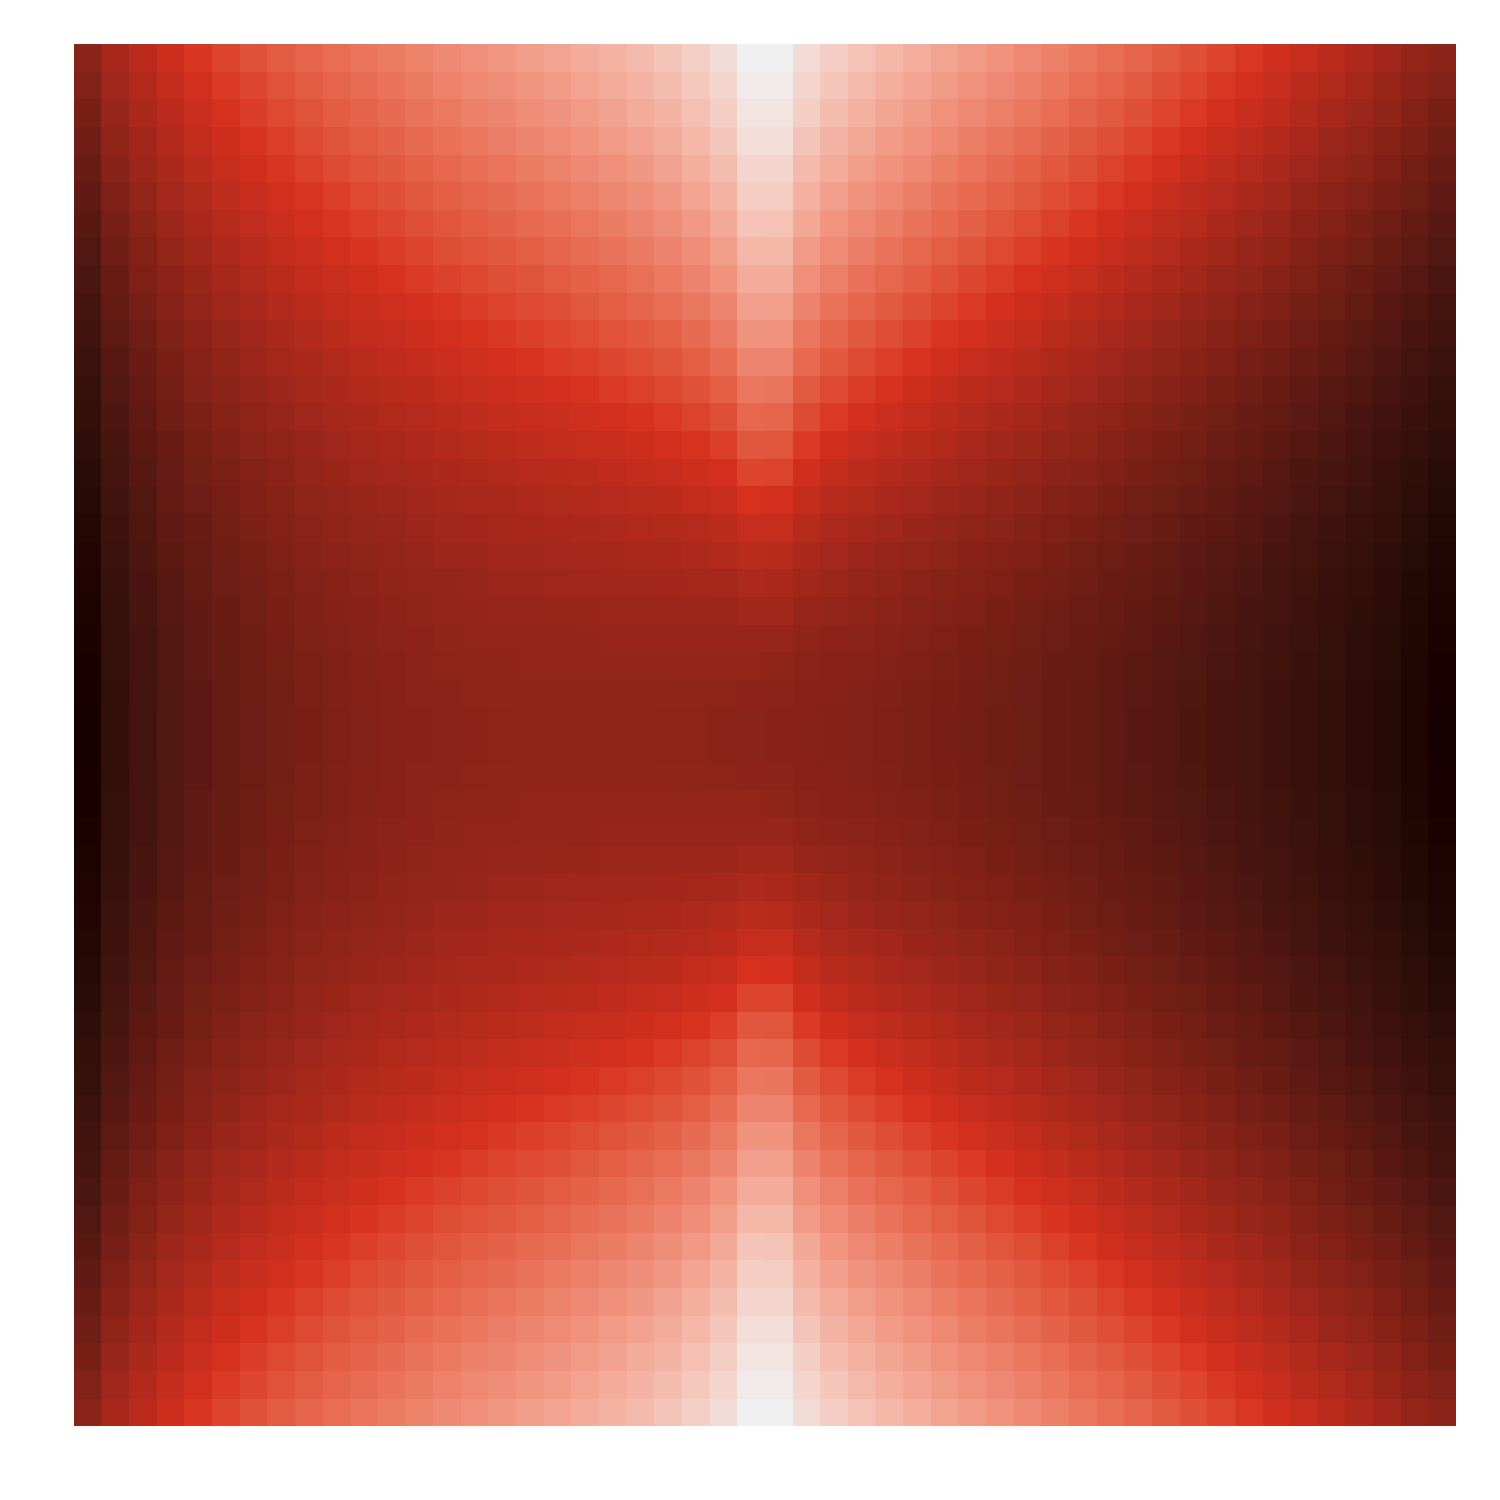
\includegraphics[width=\linewidth]{figures/p_smooth6}\\
		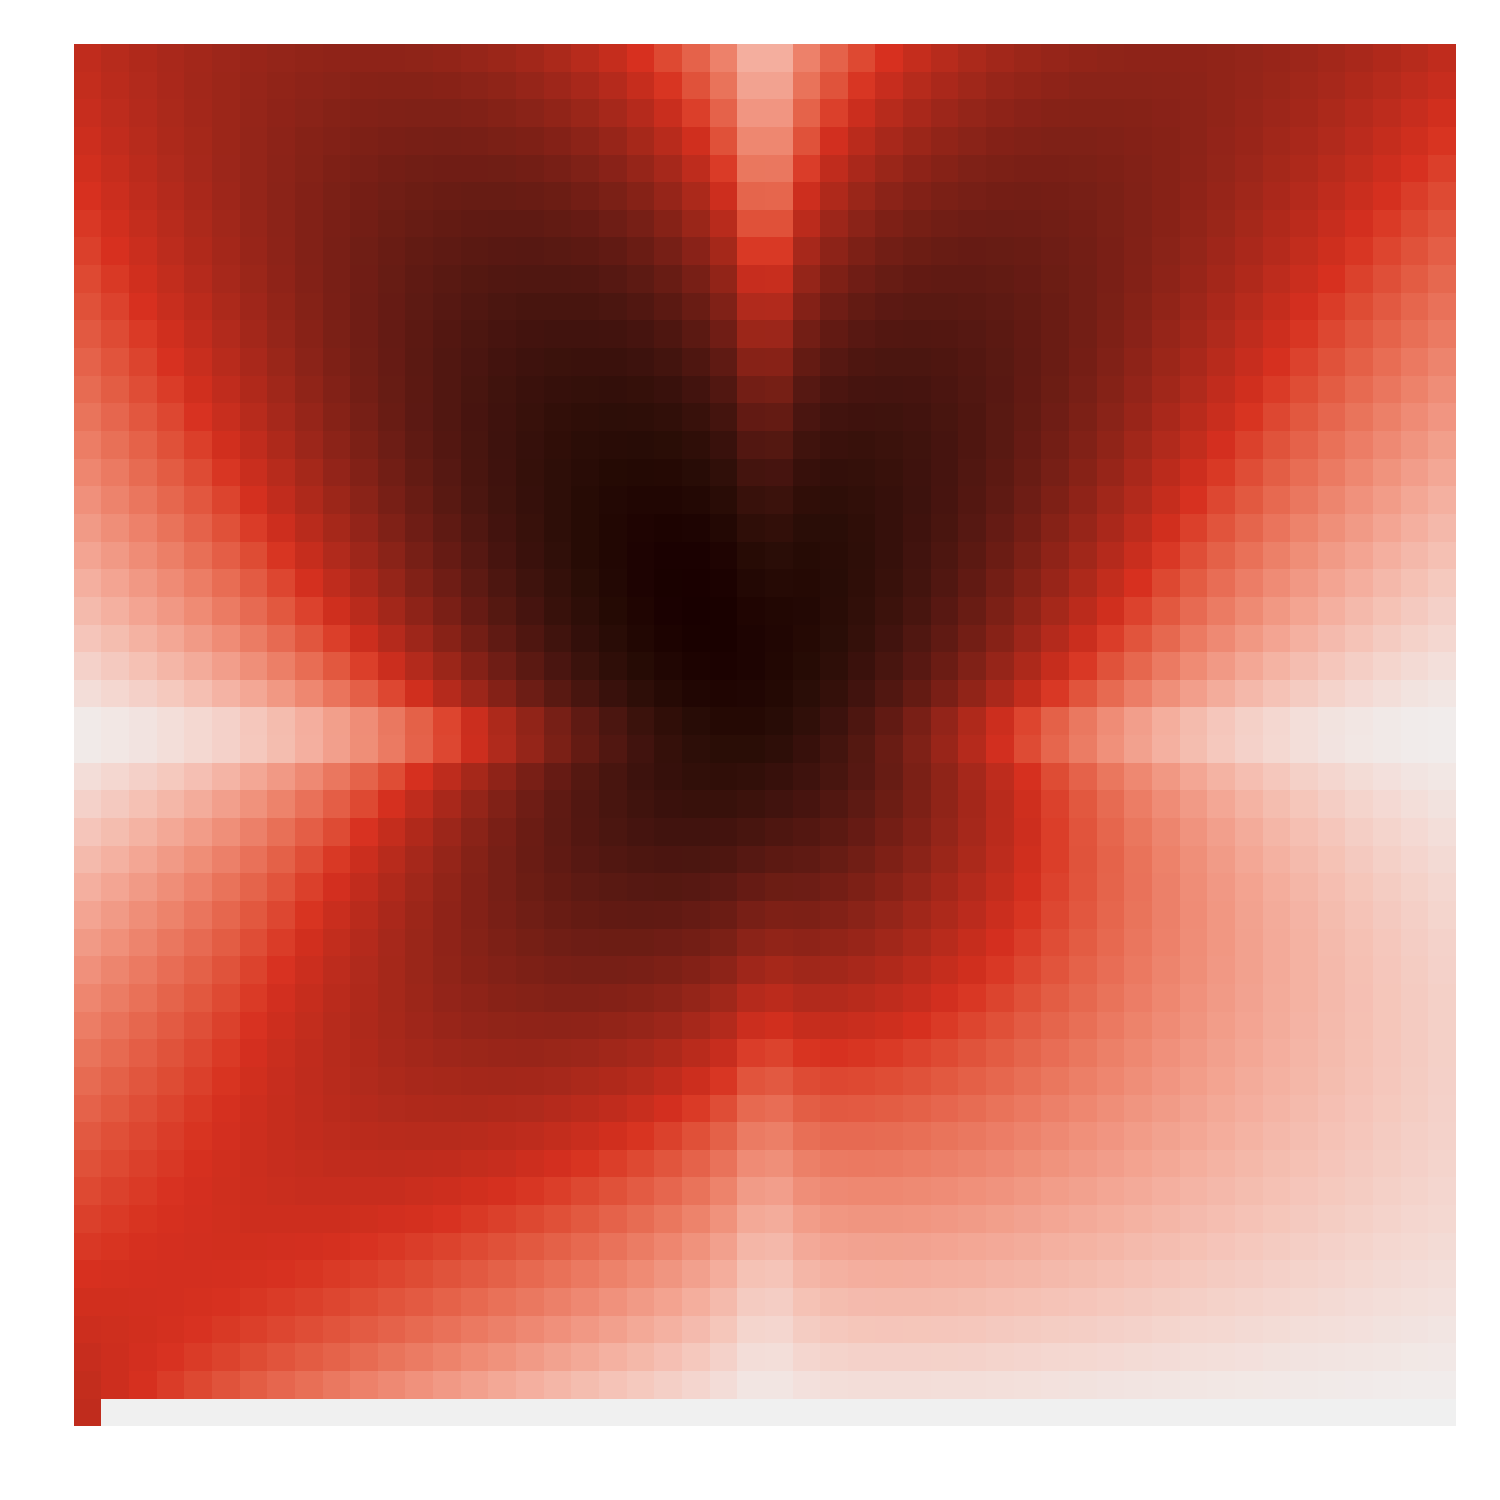
\includegraphics[width=\linewidth]{figures/p_smooth7}\\
		%\caption{First}
	\end{subfigure}
	\begin{subfigure}{0.3\textwidth}
		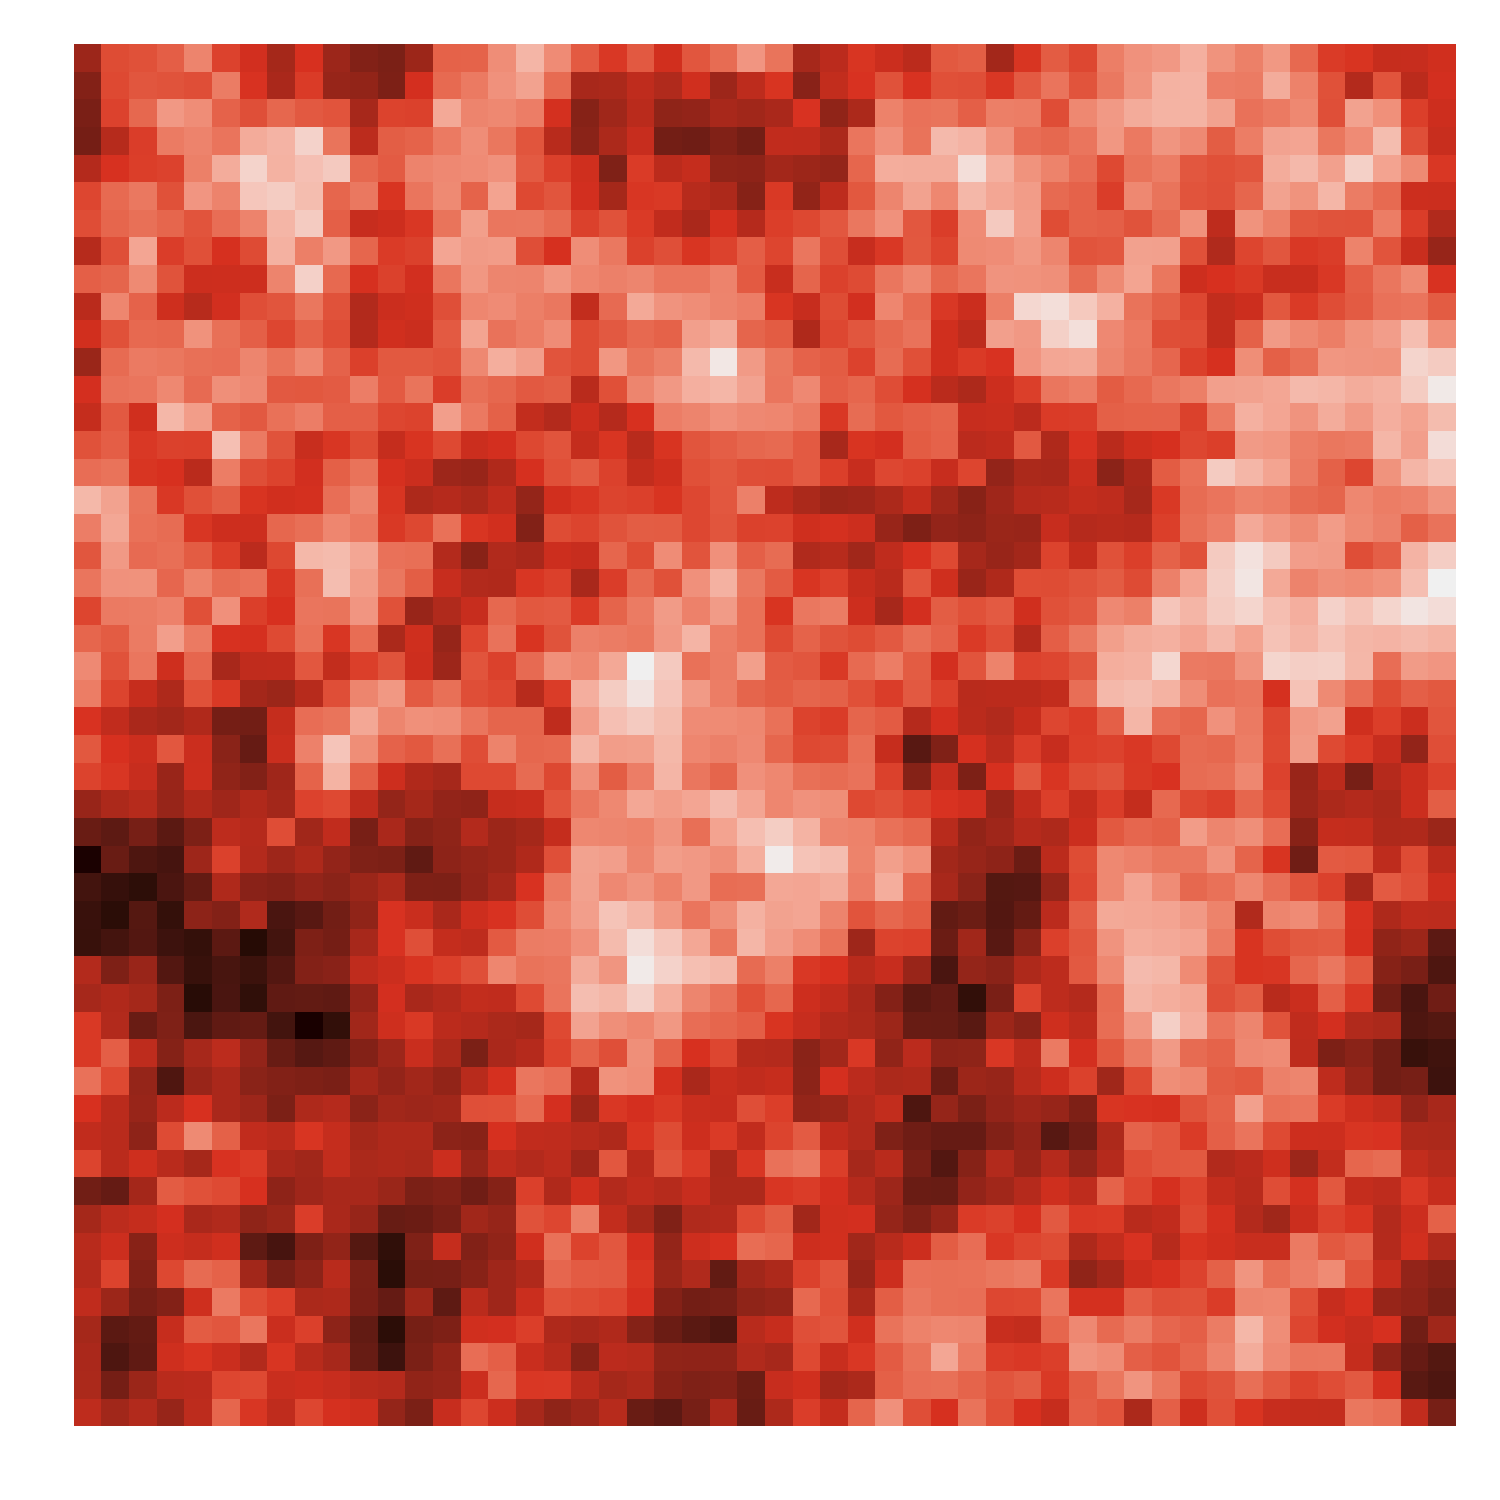
\includegraphics[width=\linewidth]{figures/p_realistic6}\\
		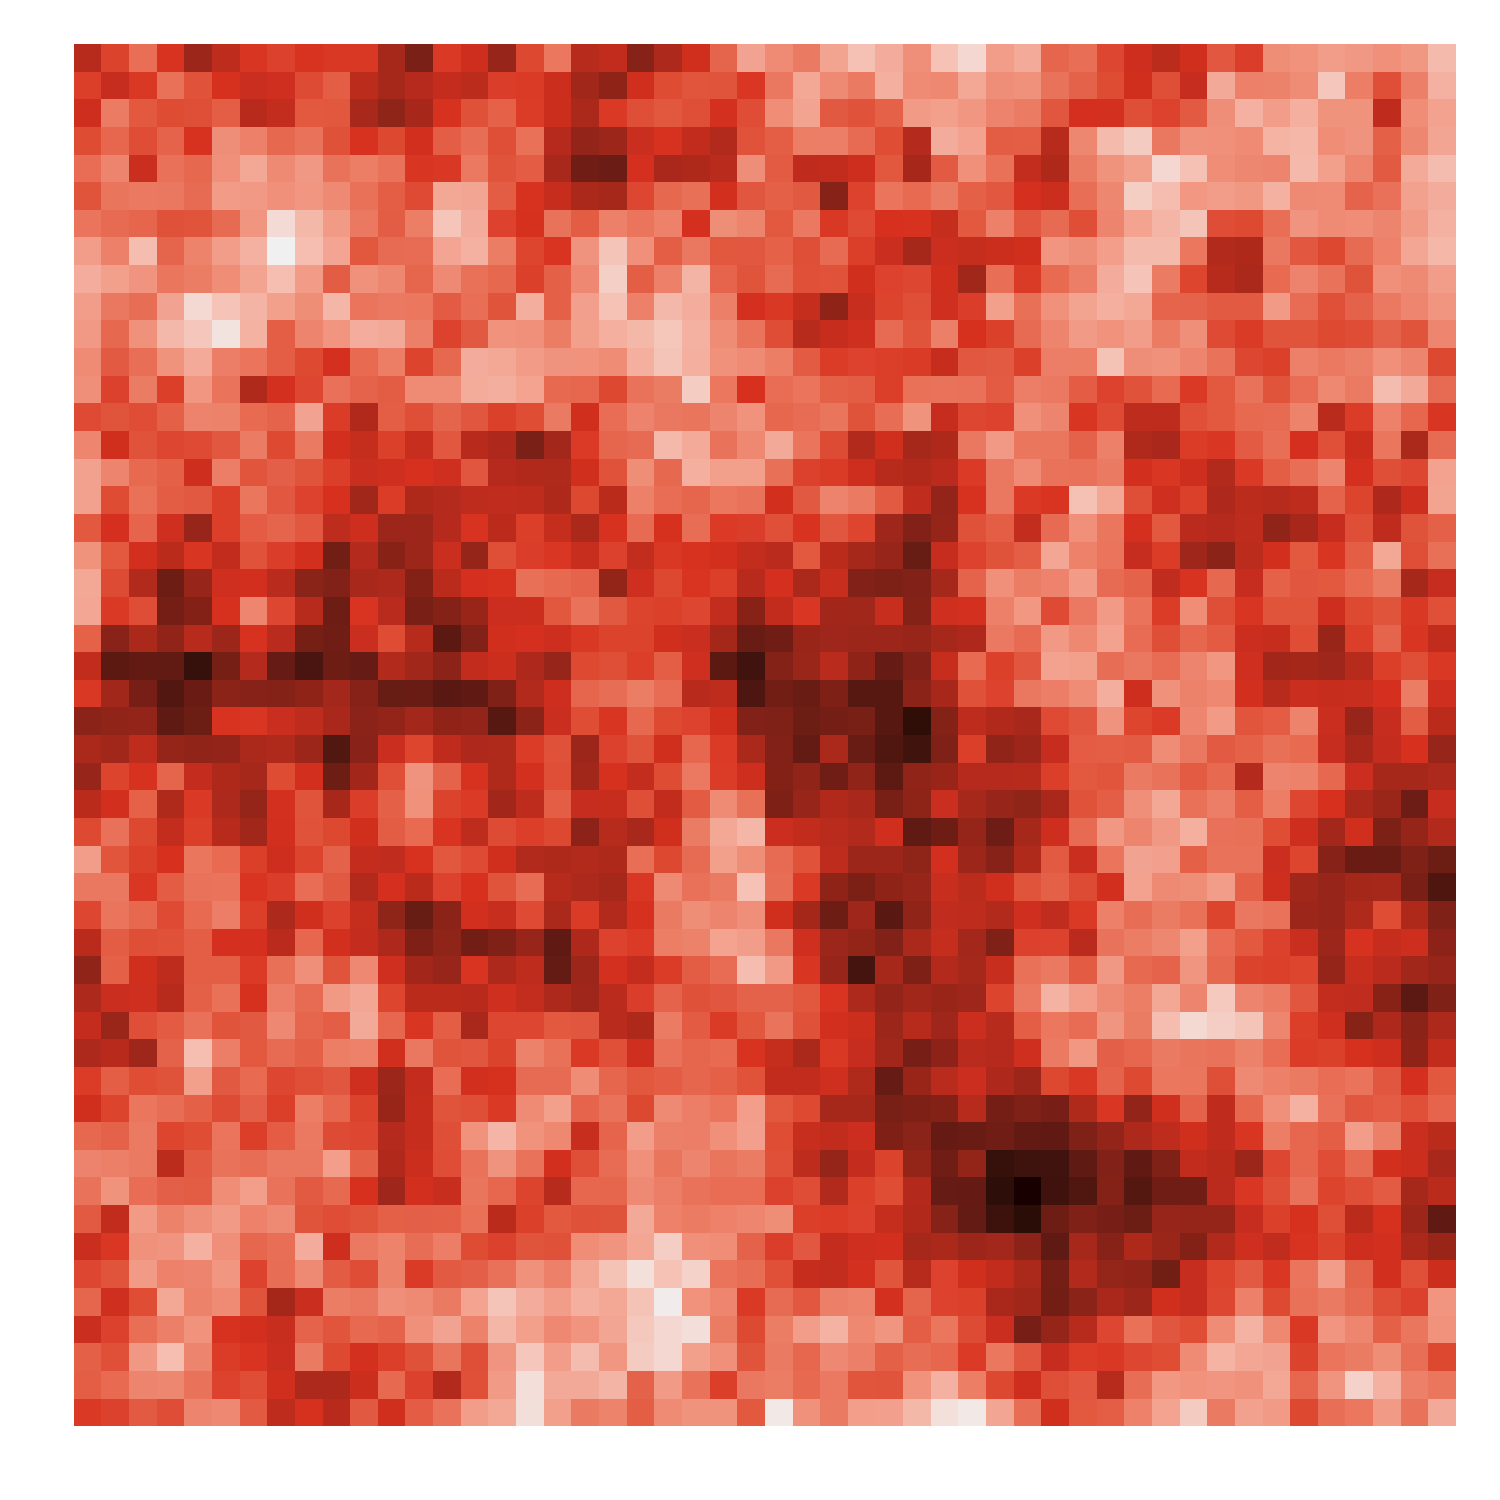
\includegraphics[width=\linewidth]{figures/p_realistic7}\\
		%\caption{First}
	\end{subfigure}
	\begin{subfigure}{0.3\textwidth}
		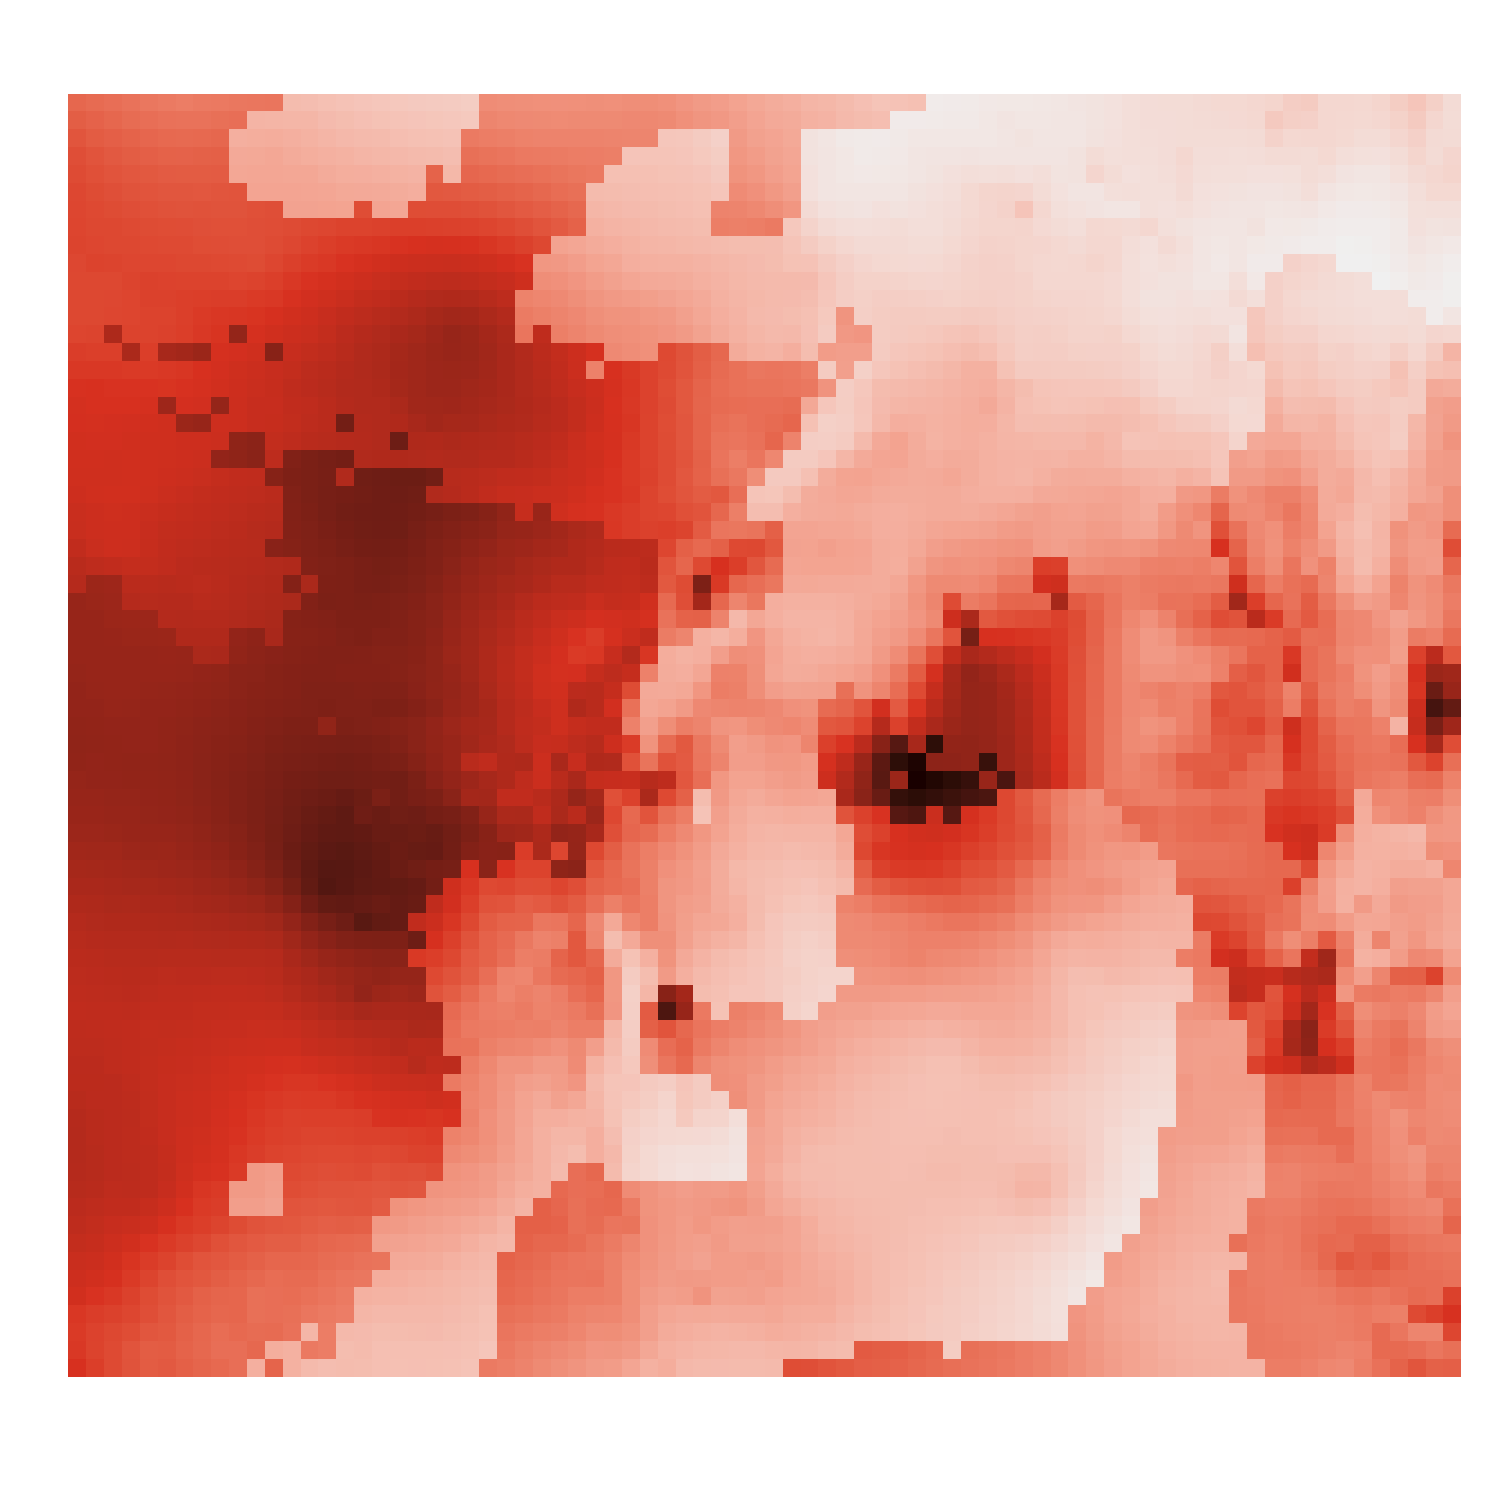
\includegraphics[width=\linewidth]{figures/p_real6}\\
		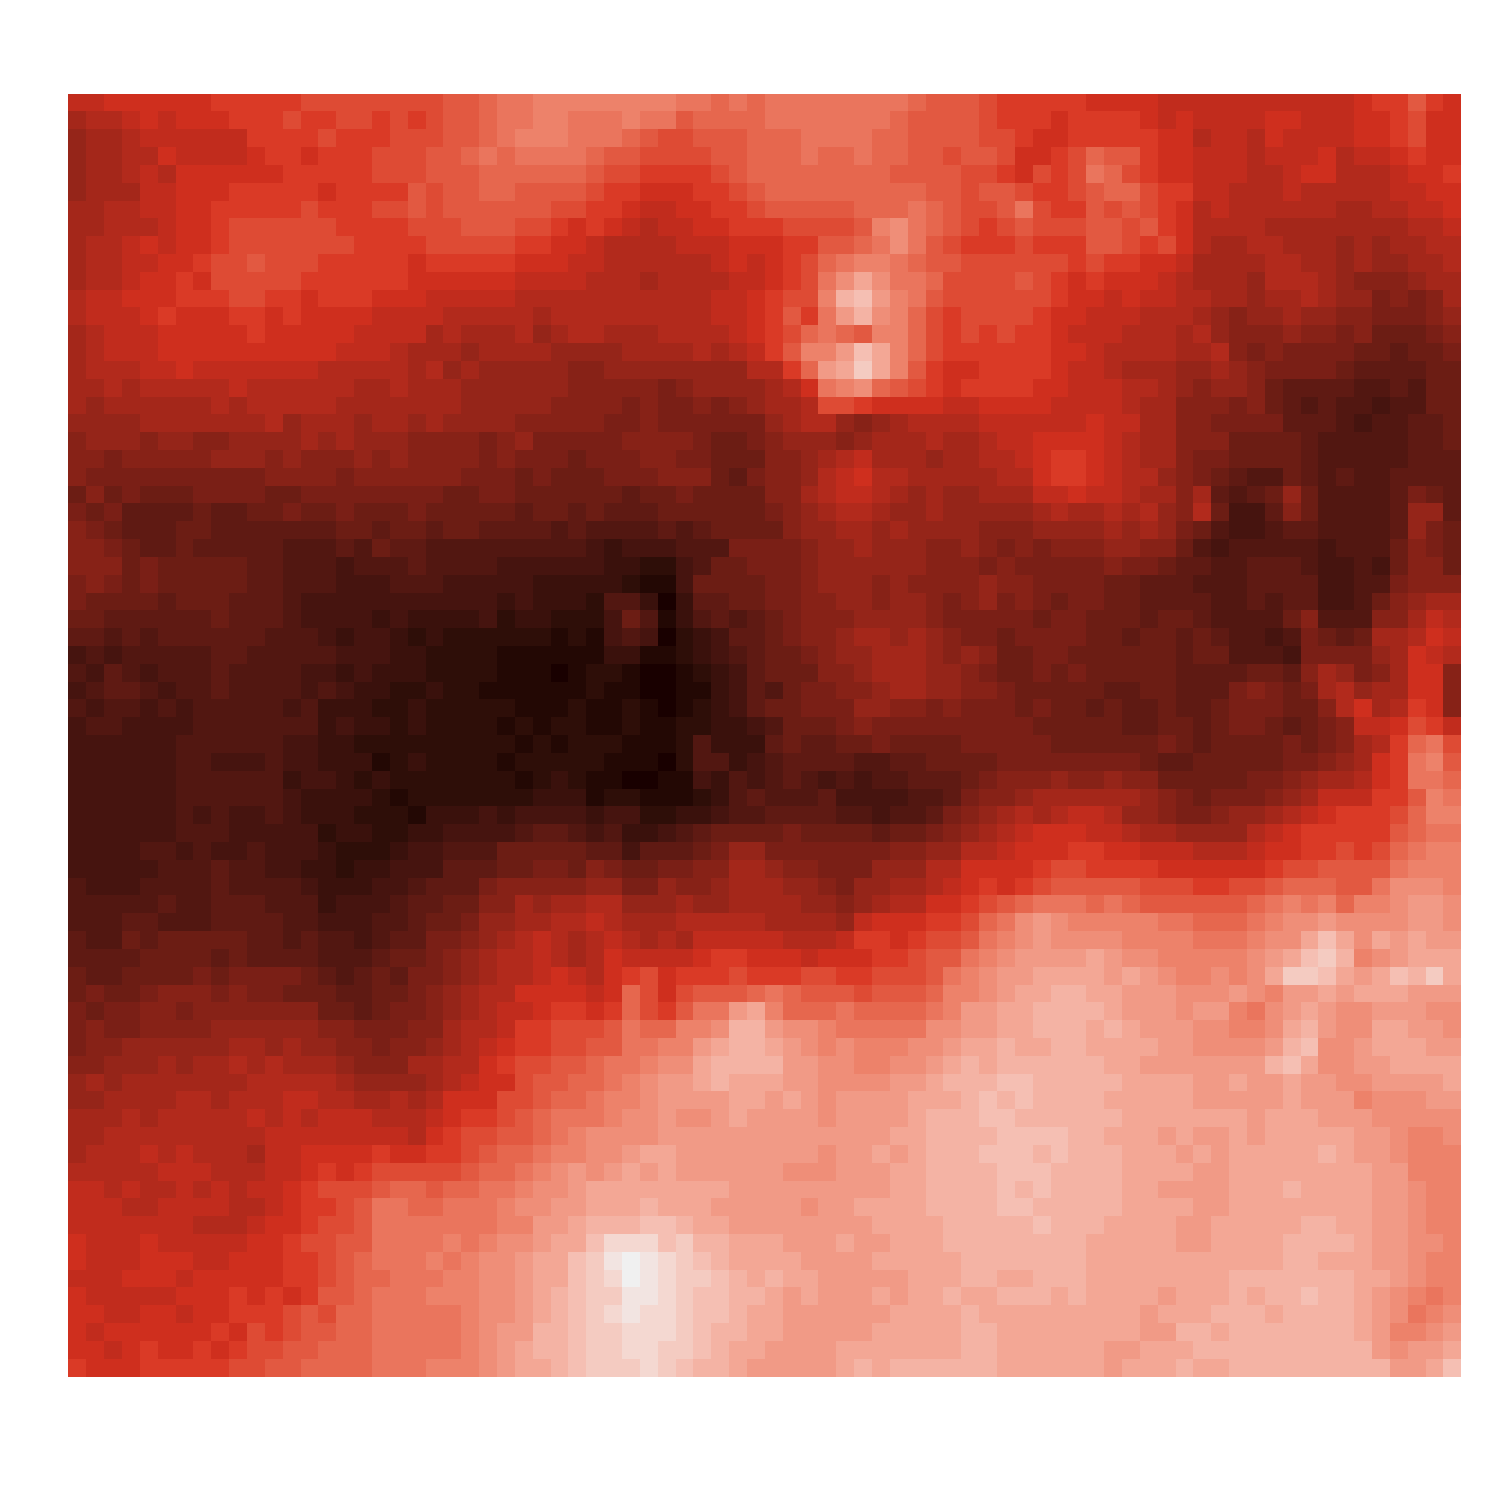
\includegraphics[width=\linewidth]{figures/p_real7}\\
		%\caption{First}
	\end{subfigure}
	\begin{subfigure}{0.08\textwidth}
		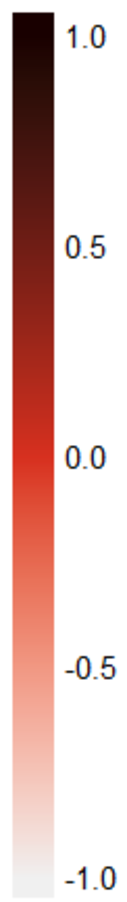
\includegraphics[width=\linewidth]{figures/legend}
		%\caption{First}
	\end{subfigure}
	 	\put(-430,160){\Large\textsc{smooth}}
	 	\put(-290,160){\Large\textsc{realistic}}
	 	\put(-135,160){\Large\textsc{real}}
	 	\put(-495,140){\Large{$x_6$}}
	 	\put(-495,-8){\Large{$x_7$}}
	 	\addtocounter{figure}{-1}
	\caption{Maps of simulated smooth (1st) and realistic (2nd) and real world (3rd column) landscapes on (simulated) Longitude (lon) / Latitude (lat) grid. All values were rescaled to [-1,1]. Smooth landscapes have the functional forms of $x_1 = lon$, $x_2 = lat$, $x_3 = (lon - \overline{lon})^2$, $x_4 = (lat - \overline{lat})^2$, $x_5 = x_3^{x_4}x_4^{x_3}$, $x_6 = x_1^{x_1}x_3^{x_4}$, and $x_7 = x_2^{x_1}x_4^{x_3}log(x_5 + 1))$. Realistic landscapes are simulated unconditional Gaussian random fields from an exponential covariance model with variance = 0.1 and scale = 0.1. The real landscapes are bio-climatic variables downloaded from \url{http://www.worldclim.org} and cropped to the extent of 5N24E to 7S37E, with $x_1 =$ annual mean temperature, $x_2 =$ precipitation of coldest quarter, $x_3 =$ mean diurnal range, $x_4 =$ annual precipitation, $x_5 =$ temperature seasonality, $x_6 =$ precipitation of warmest quarter, and $x_7 =$ isothermality. The grid sizes for the simulated landscapes are 50 $\times$ 50 cells, and for the real landscape 72 $\times$ 78 cells.
		\label{predictor_maps}}
\end{figure}

\begin{figure}
	\centering
	\begin{subfigure}{0.3\textwidth}
		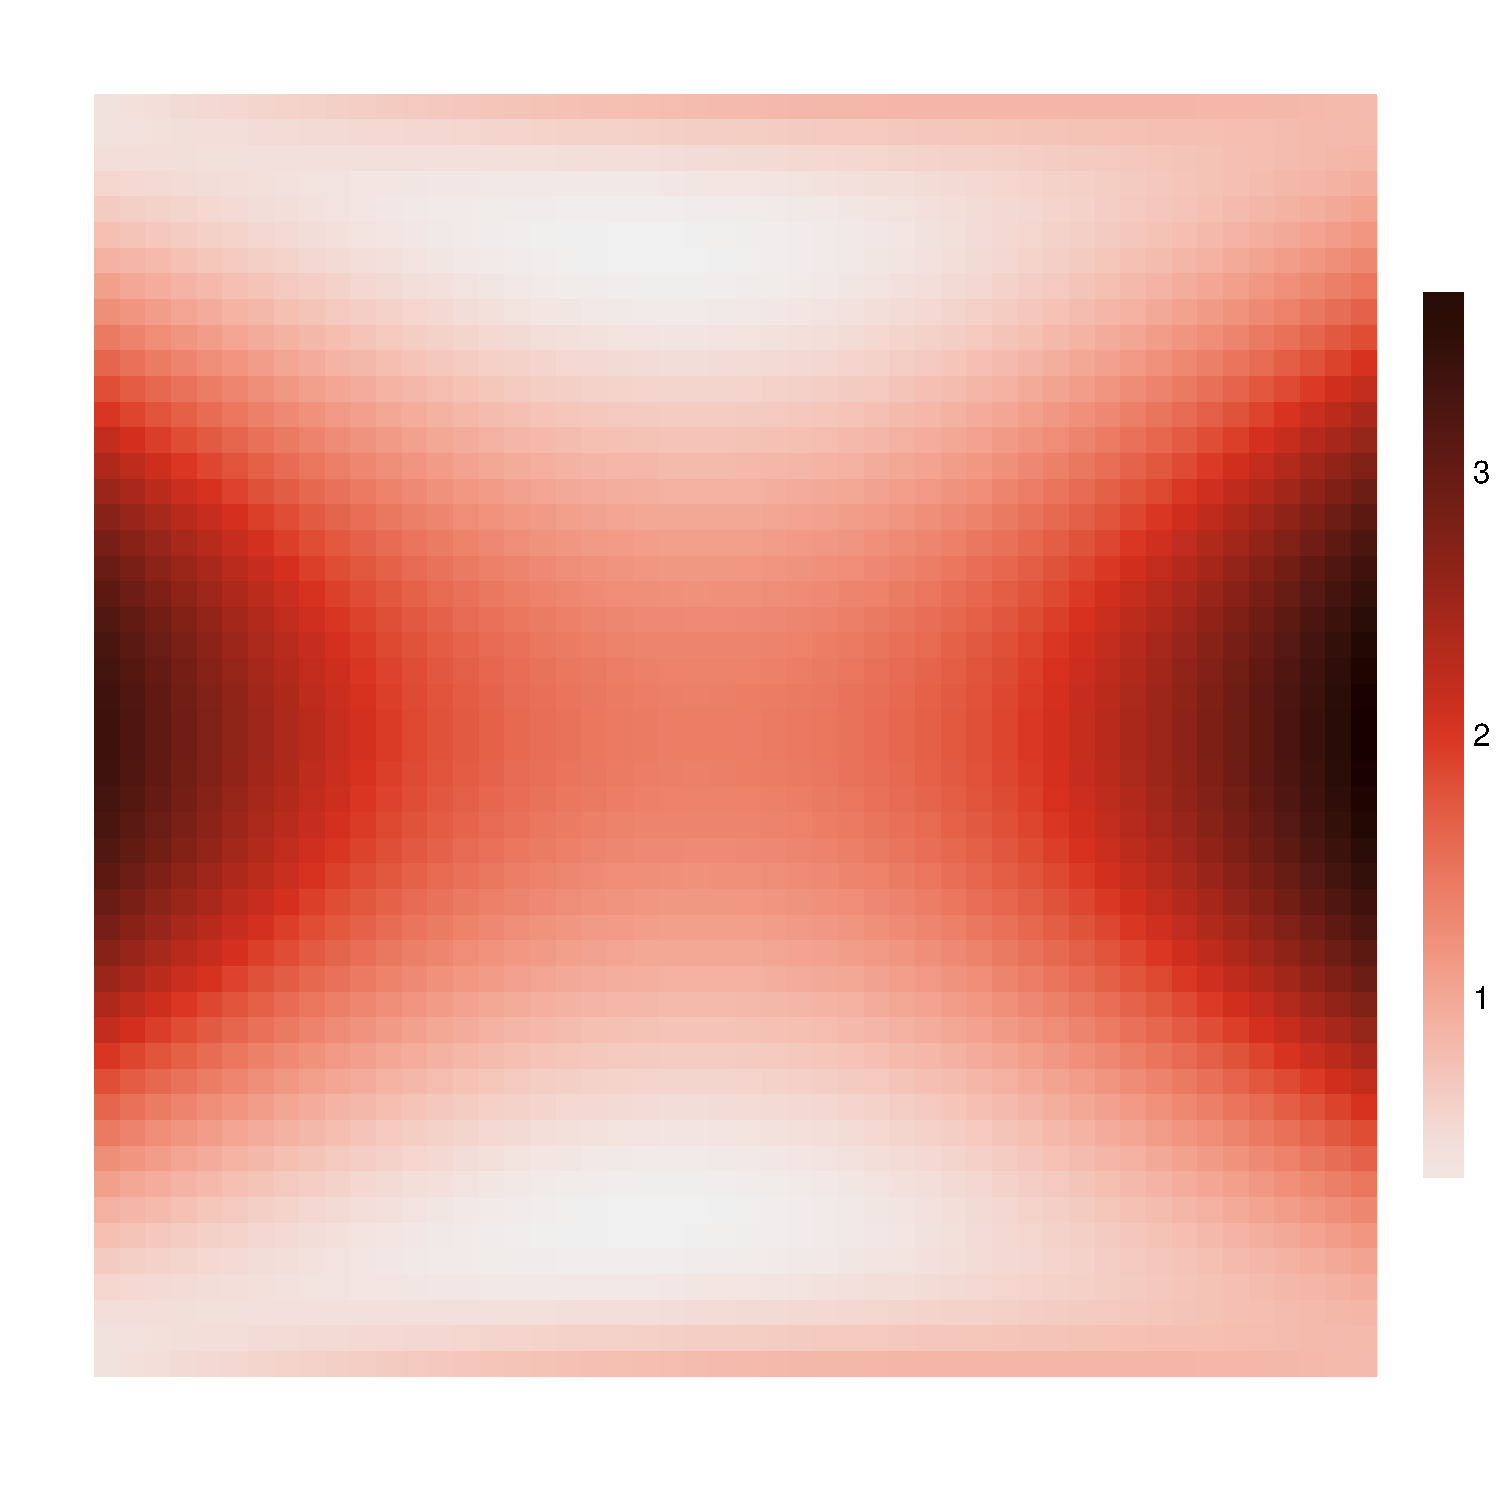
\includegraphics[width=\linewidth]{figures/y110}\\
		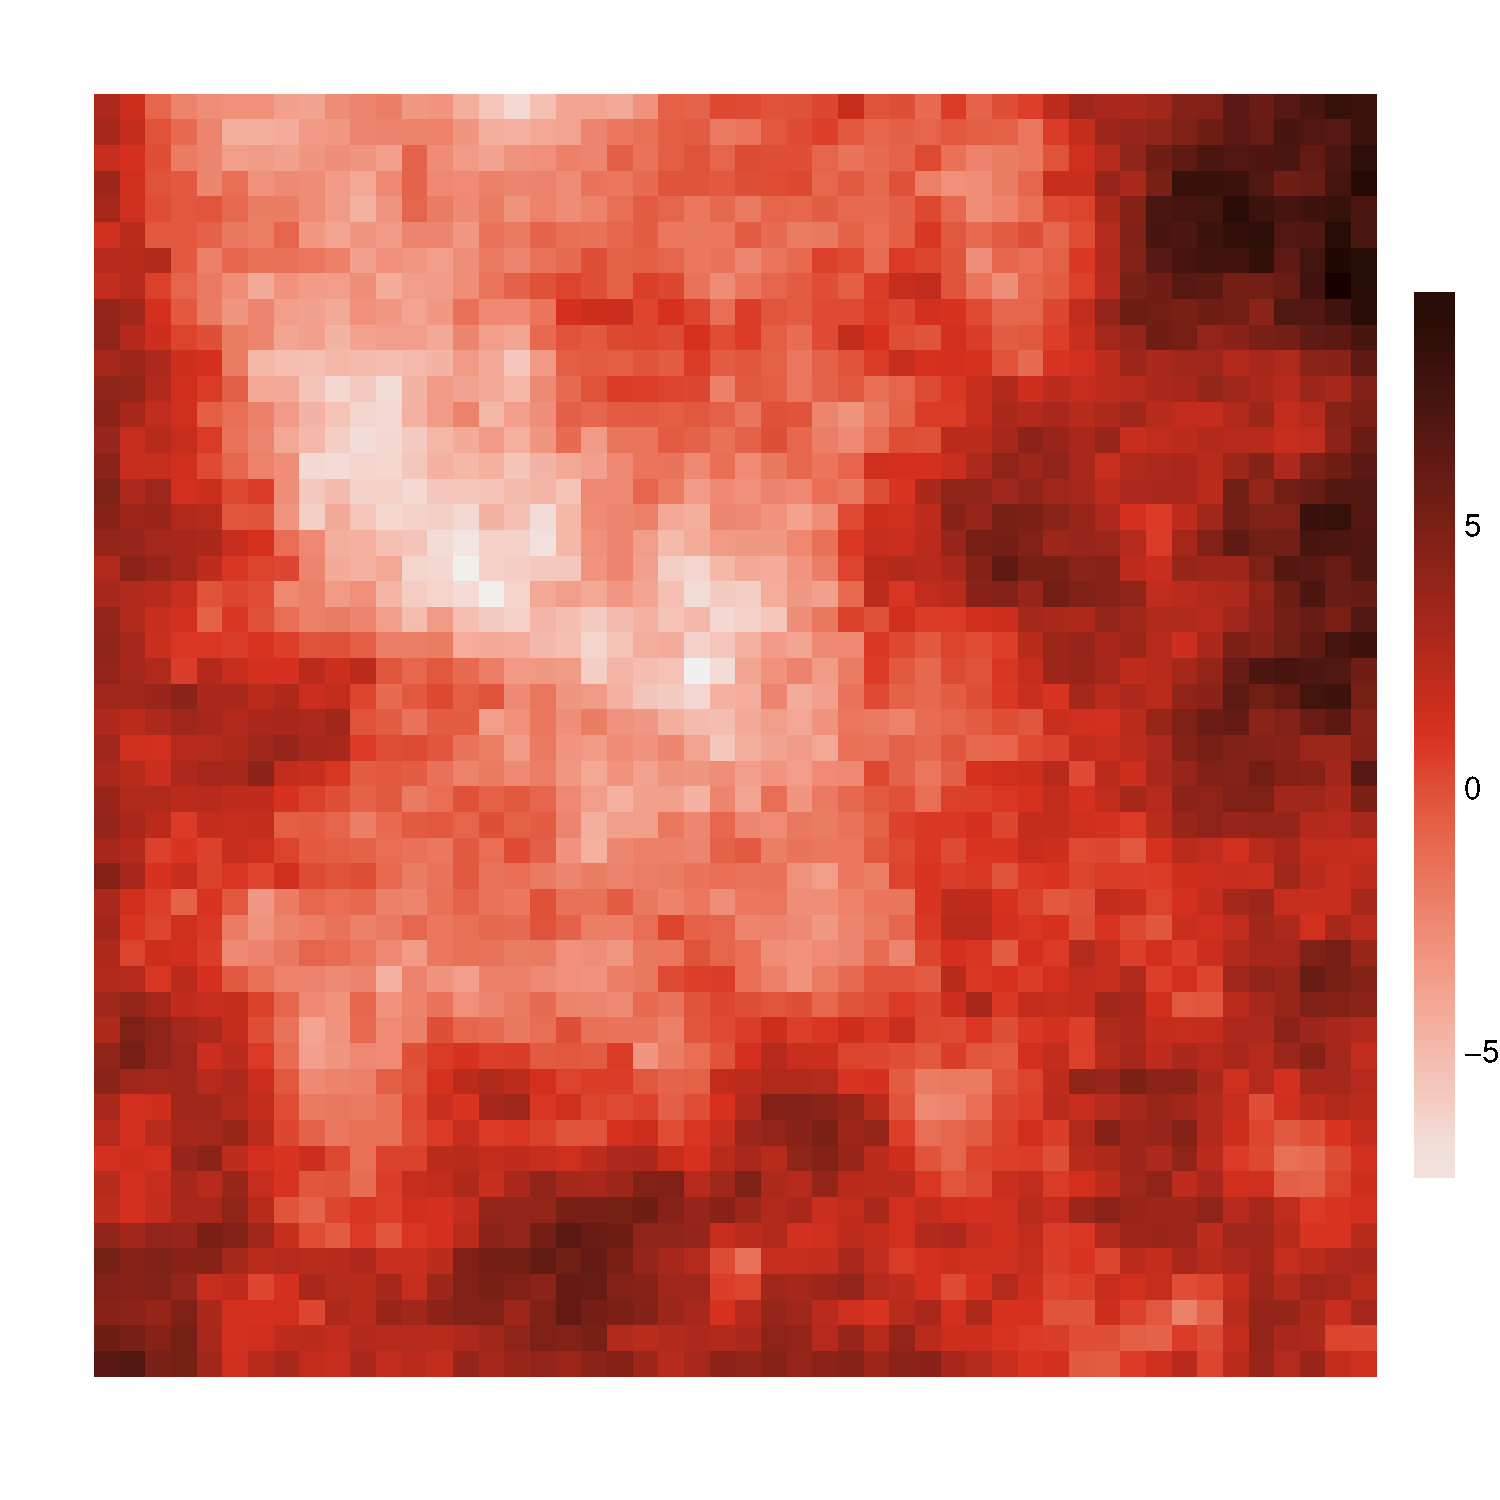
\includegraphics[width=\linewidth]{figures/y111}\\
		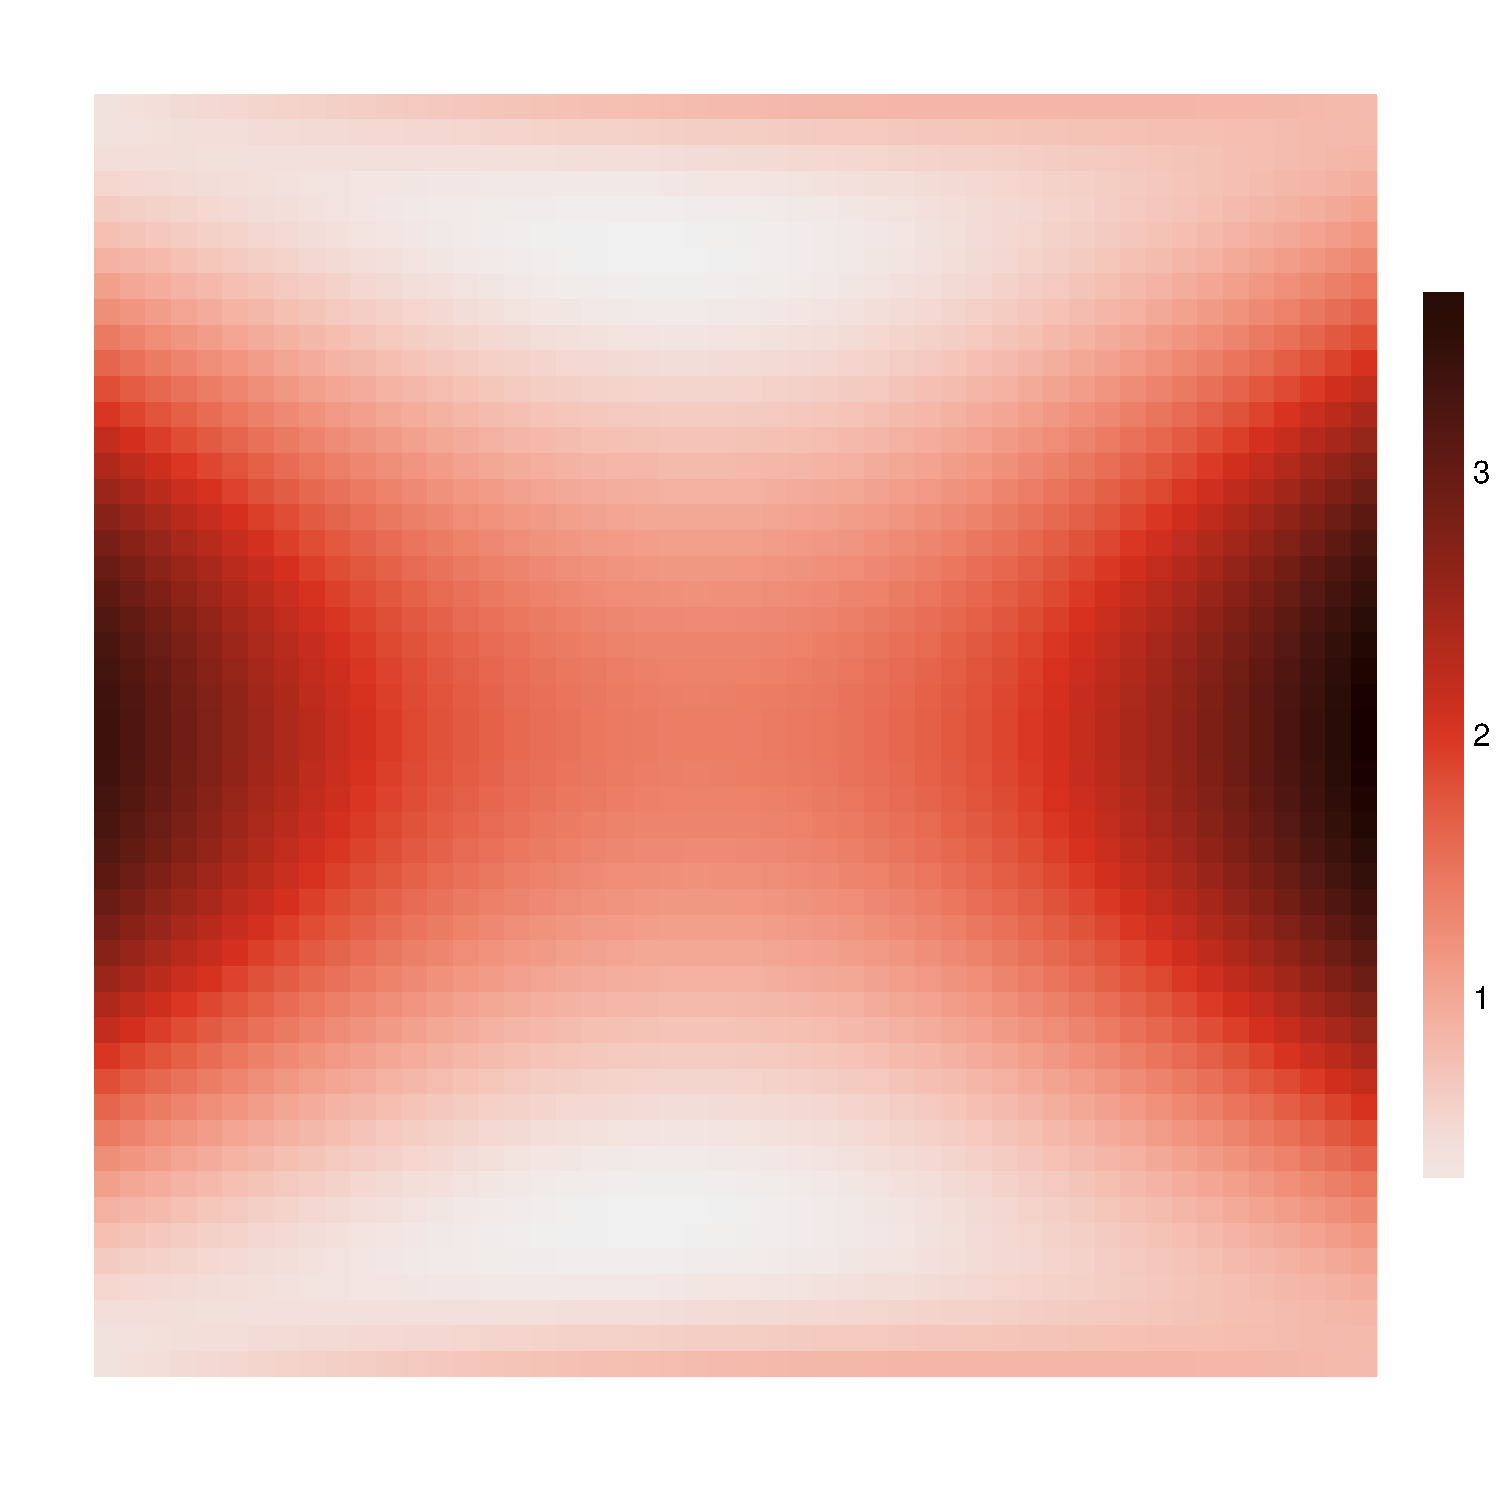
\includegraphics[width=\linewidth]{figures/y112}\\
		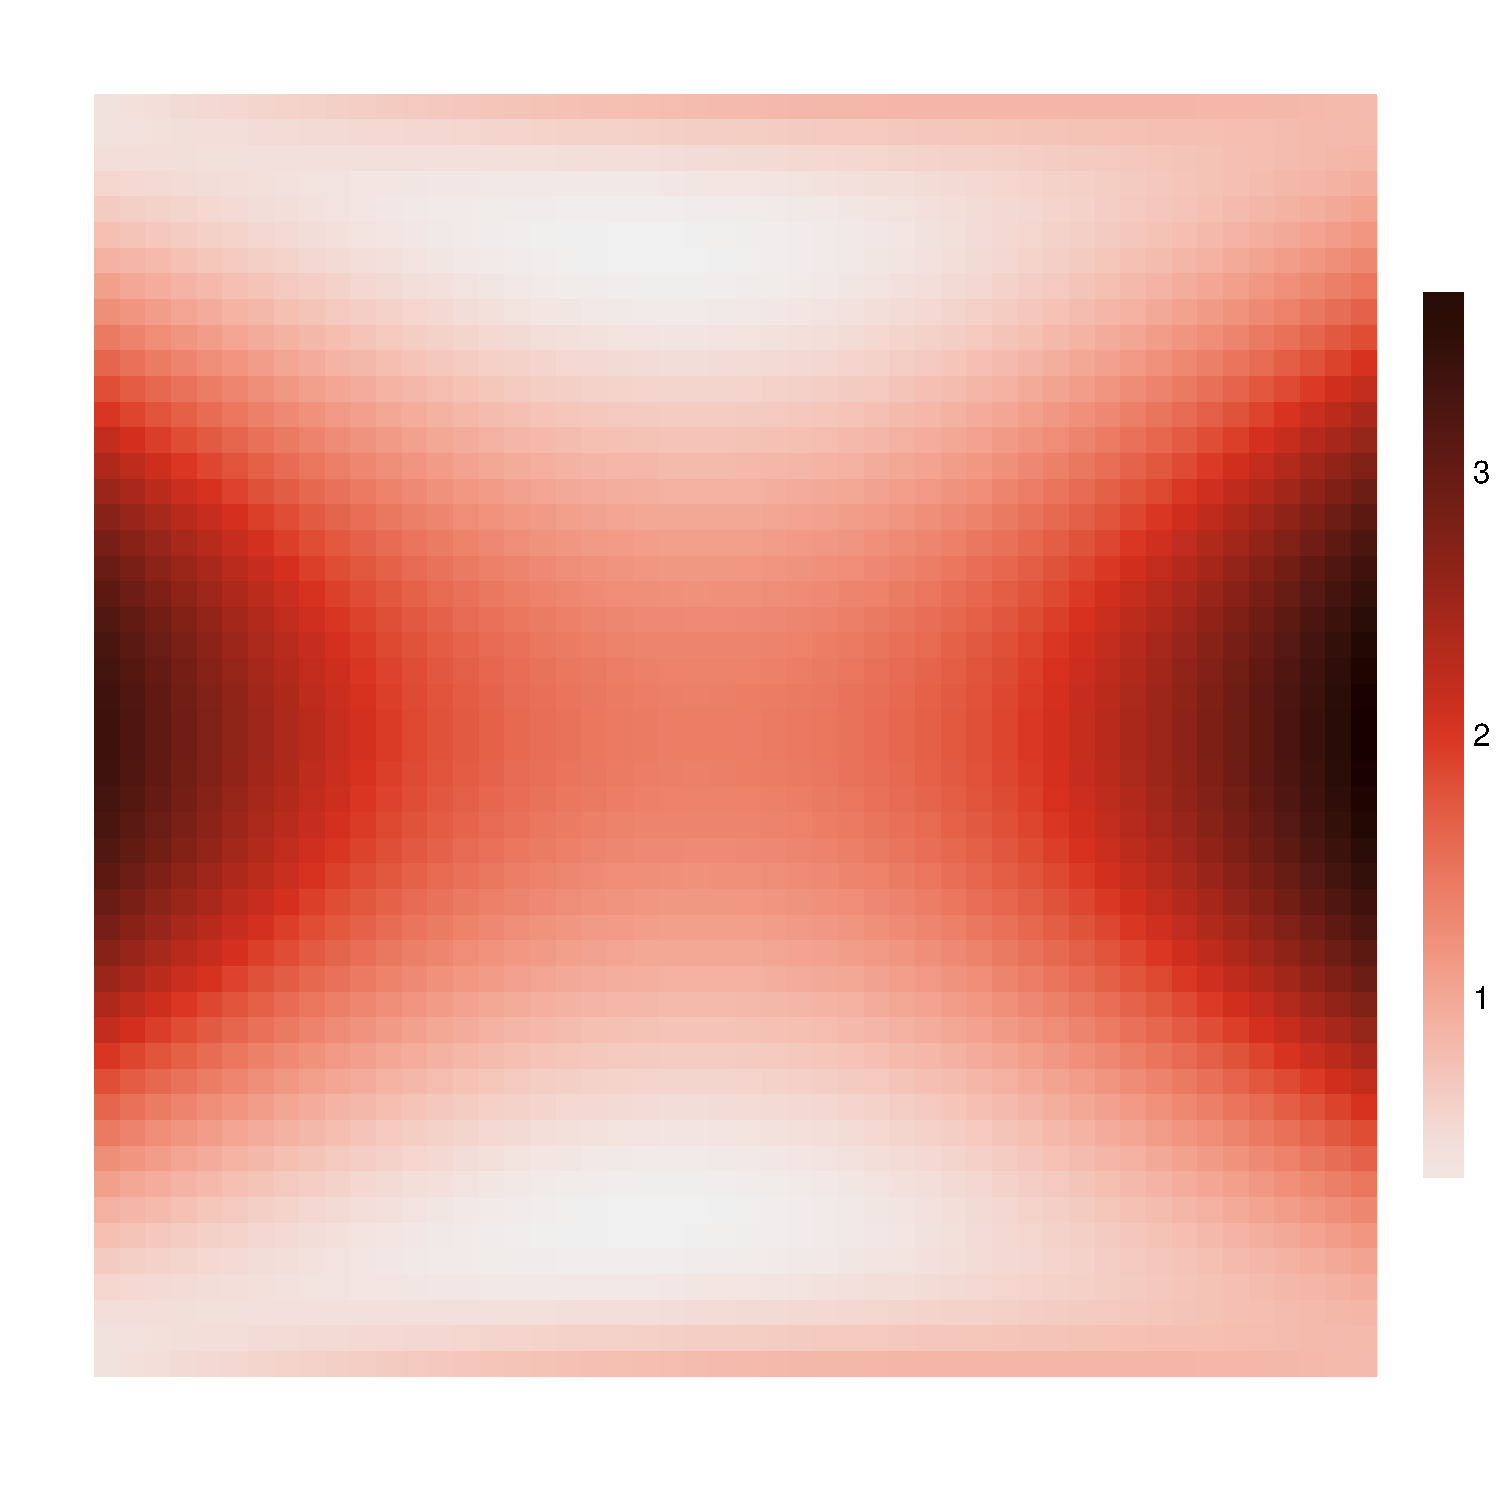
\includegraphics[width=\linewidth]{figures/y113}\\
		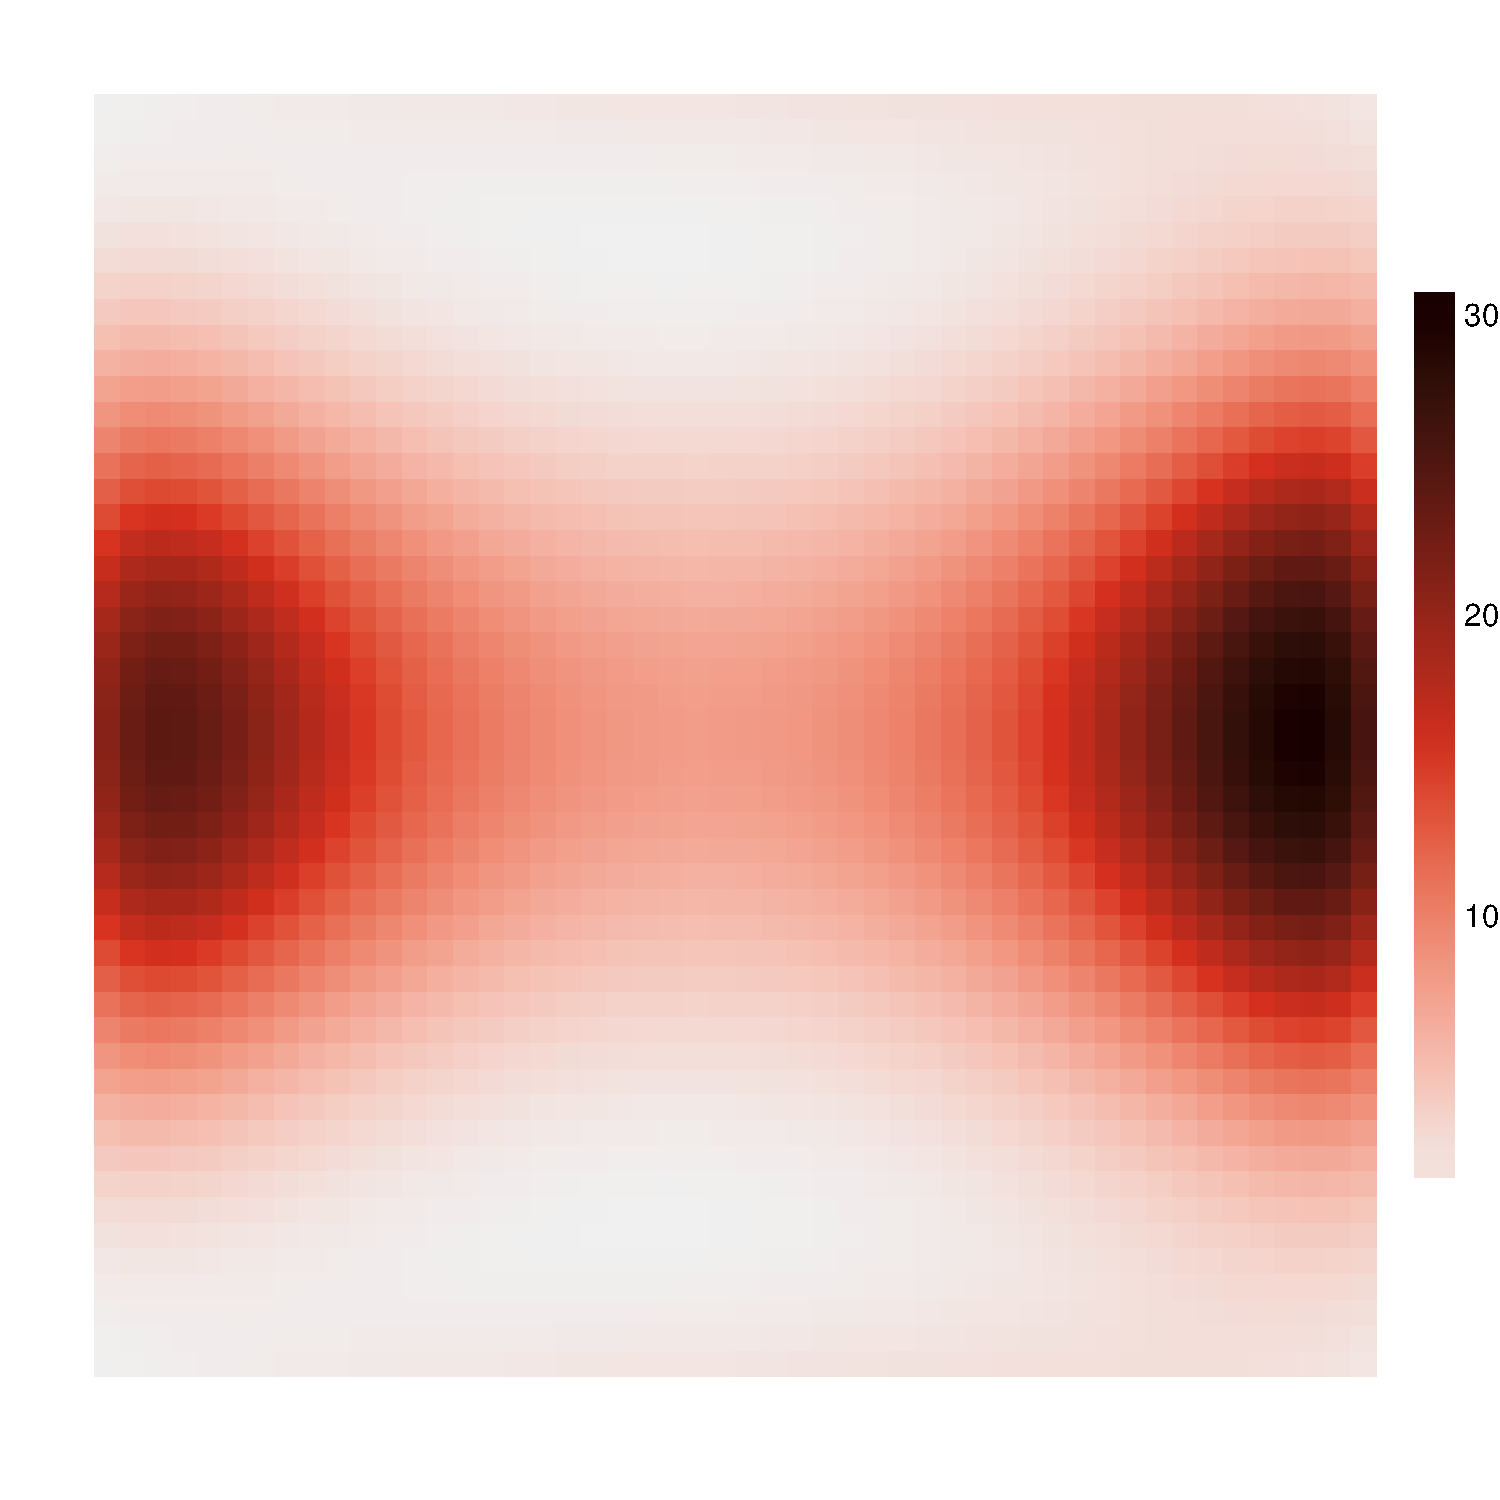
\includegraphics[width=\linewidth]{figures/y114}\\
	\end{subfigure}
	\begin{subfigure}{0.3\textwidth}
		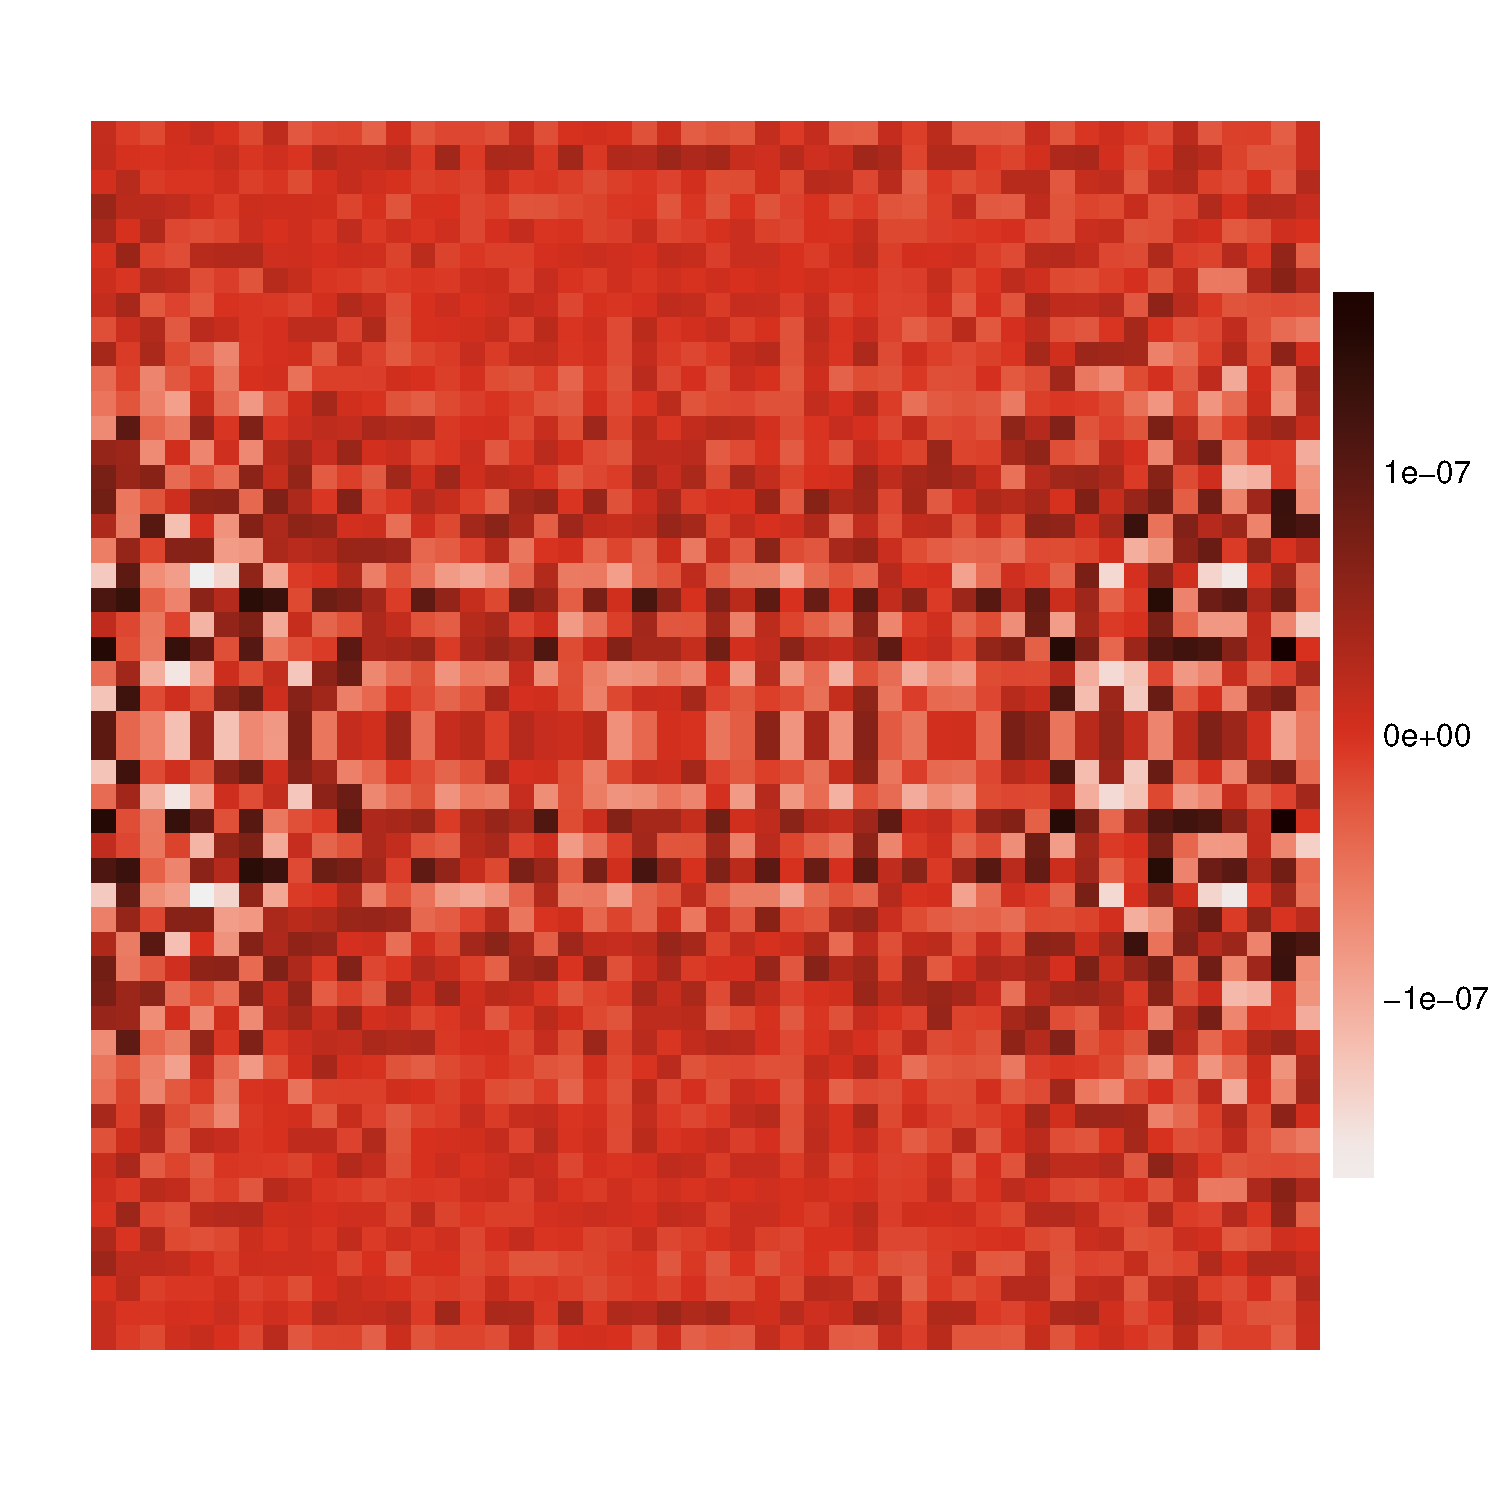
\includegraphics[width=\linewidth]{figures/res110}\\
		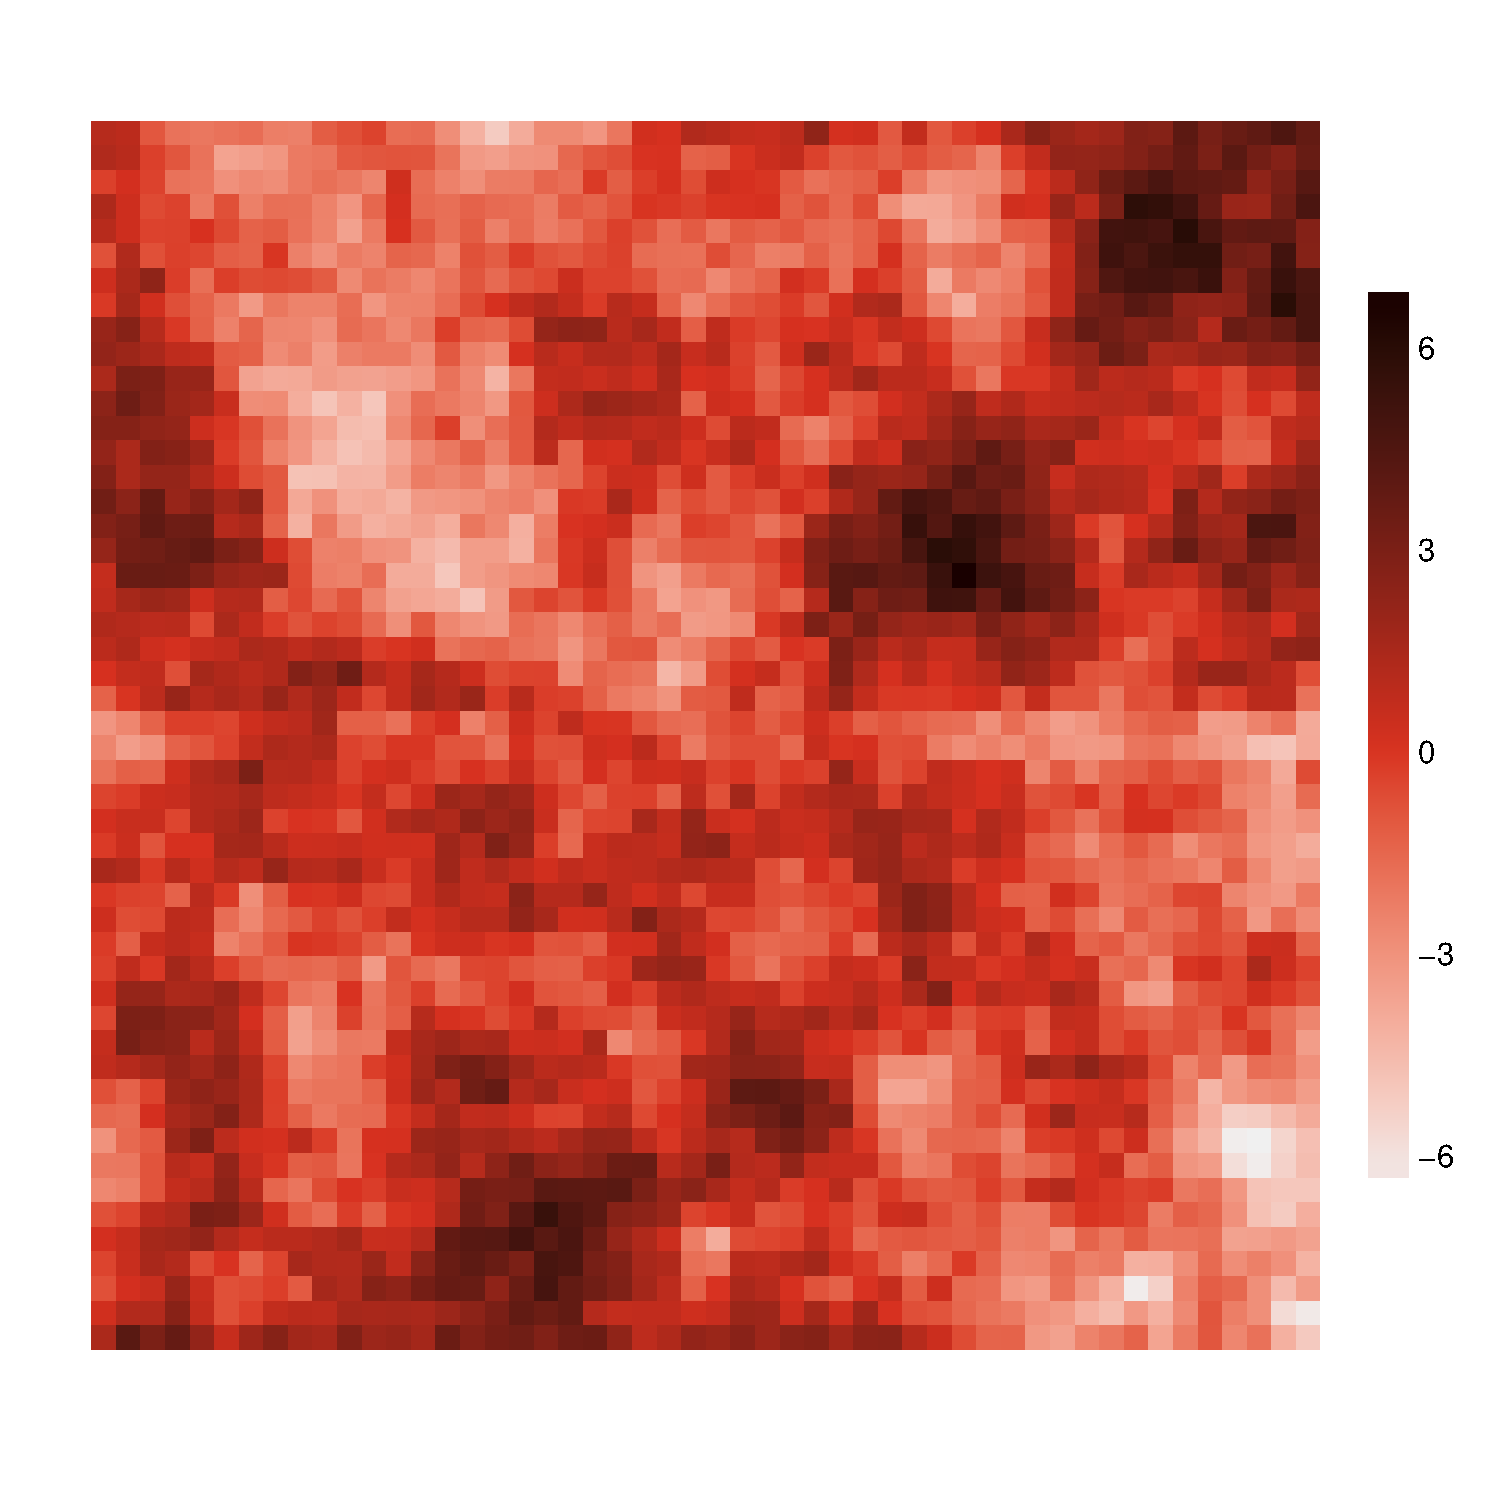
\includegraphics[width=\linewidth]{figures/res111}\\
		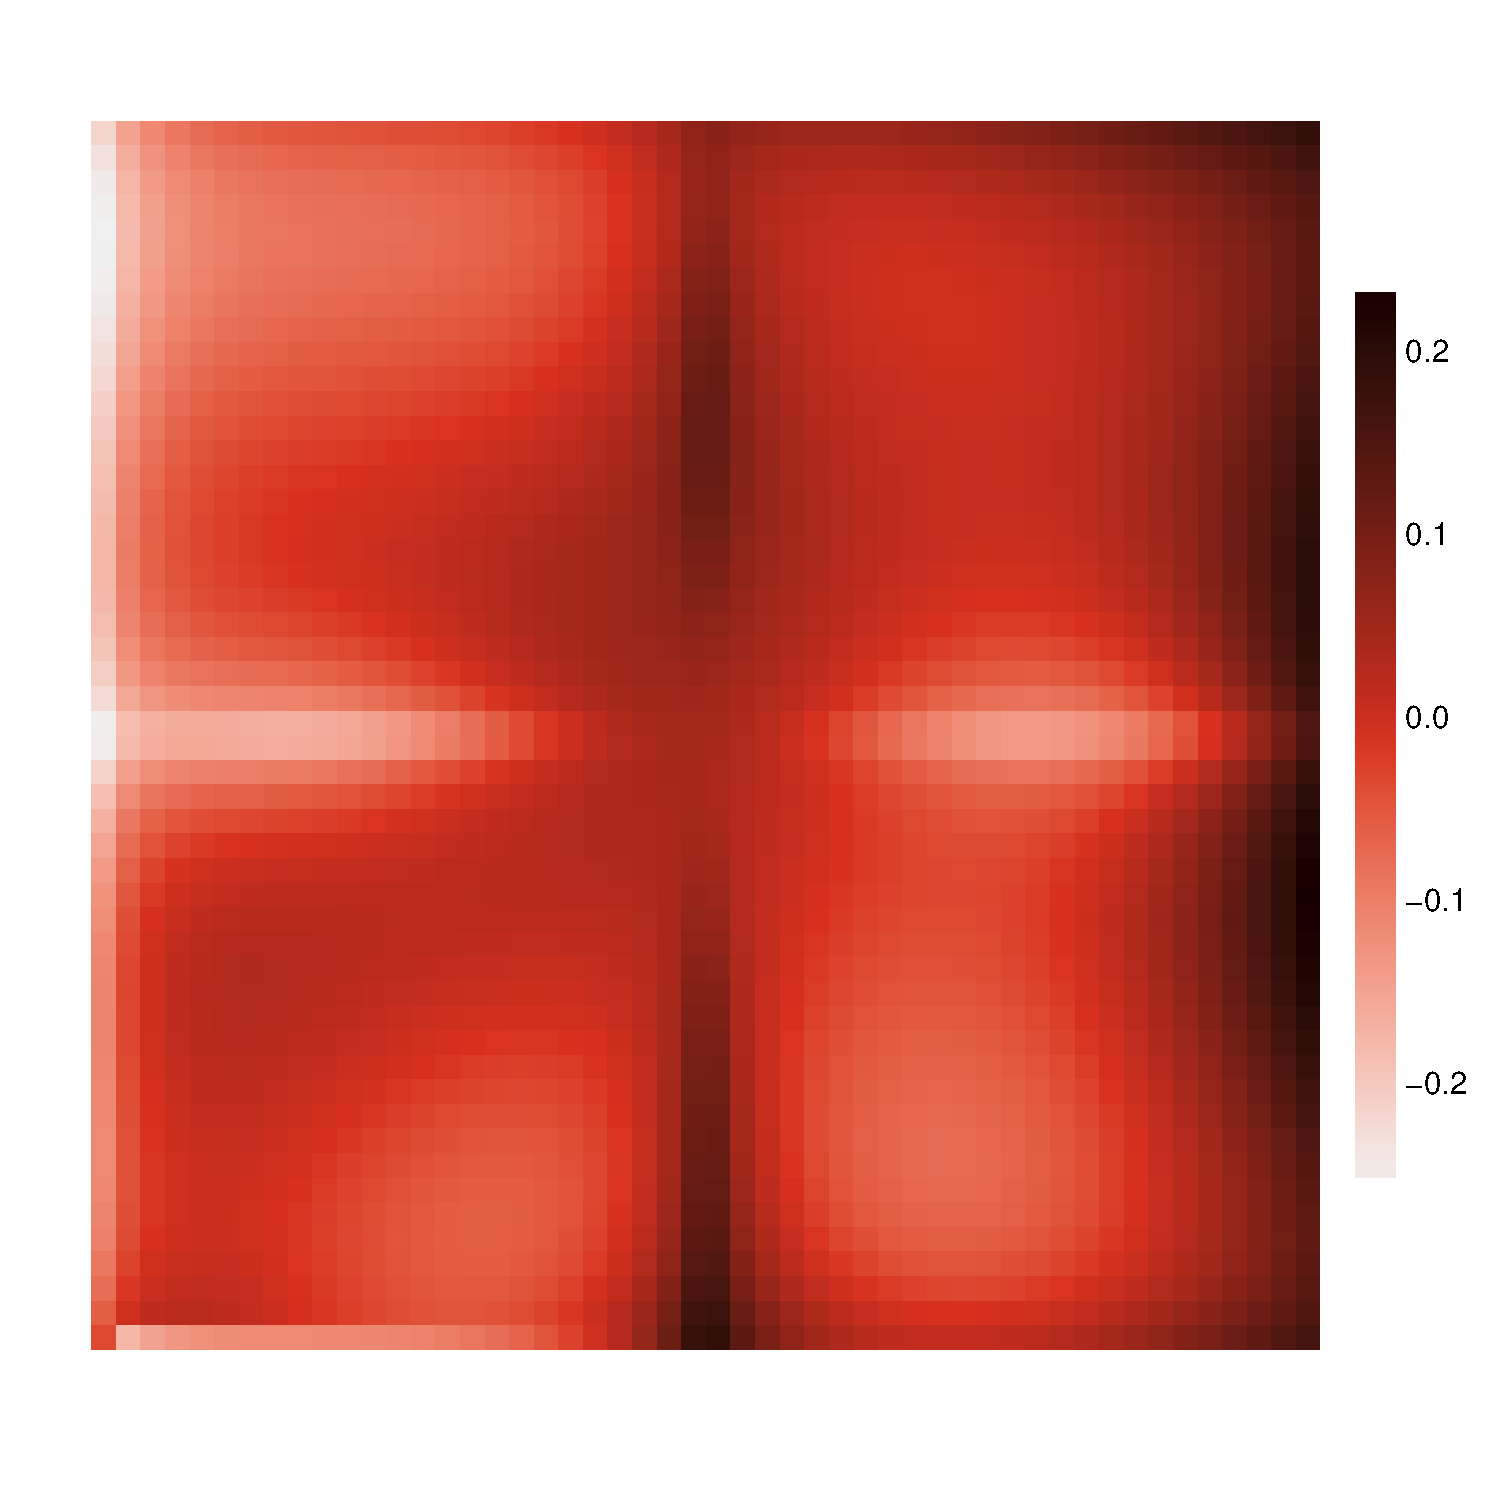
\includegraphics[width=\linewidth]{figures/res112}\\
		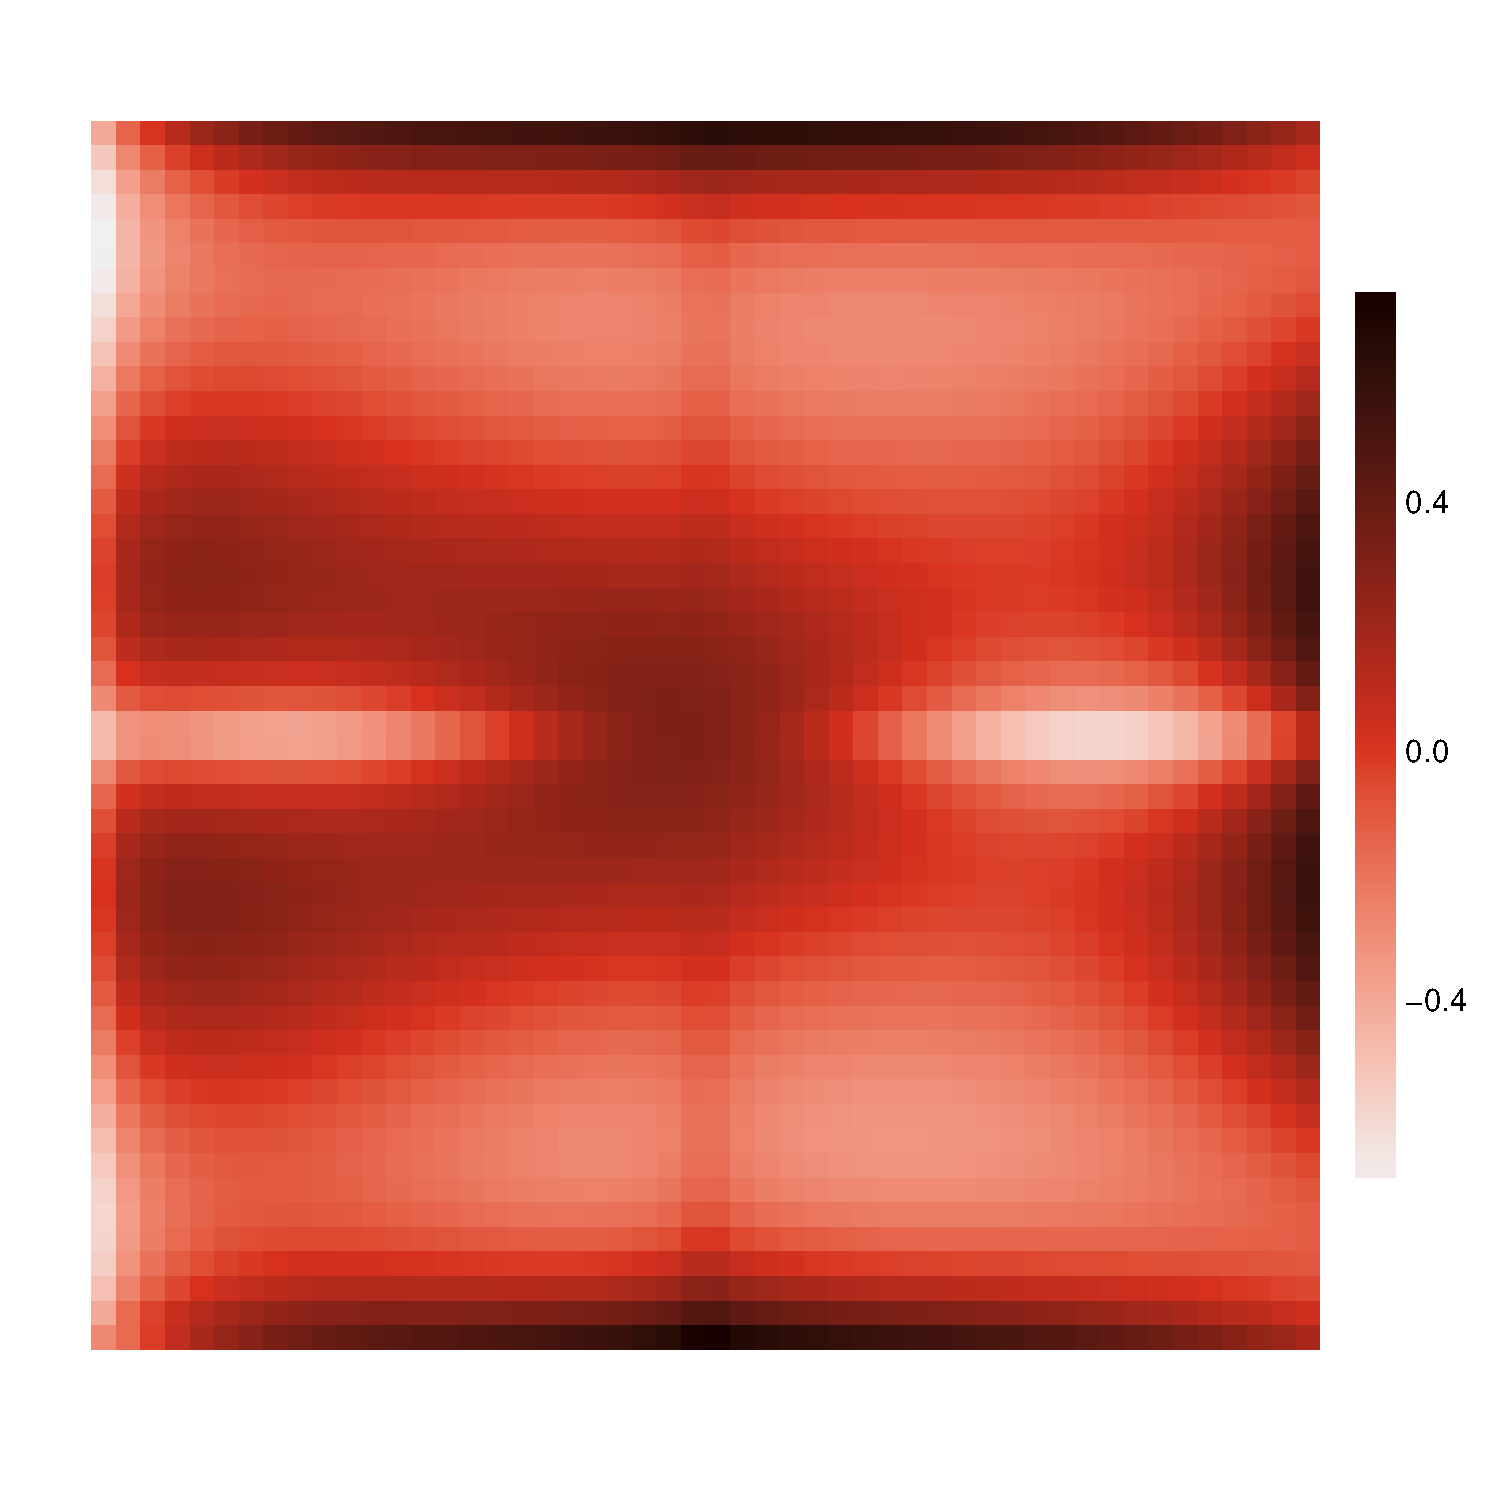
\includegraphics[width=\linewidth]{figures/res113}\\
		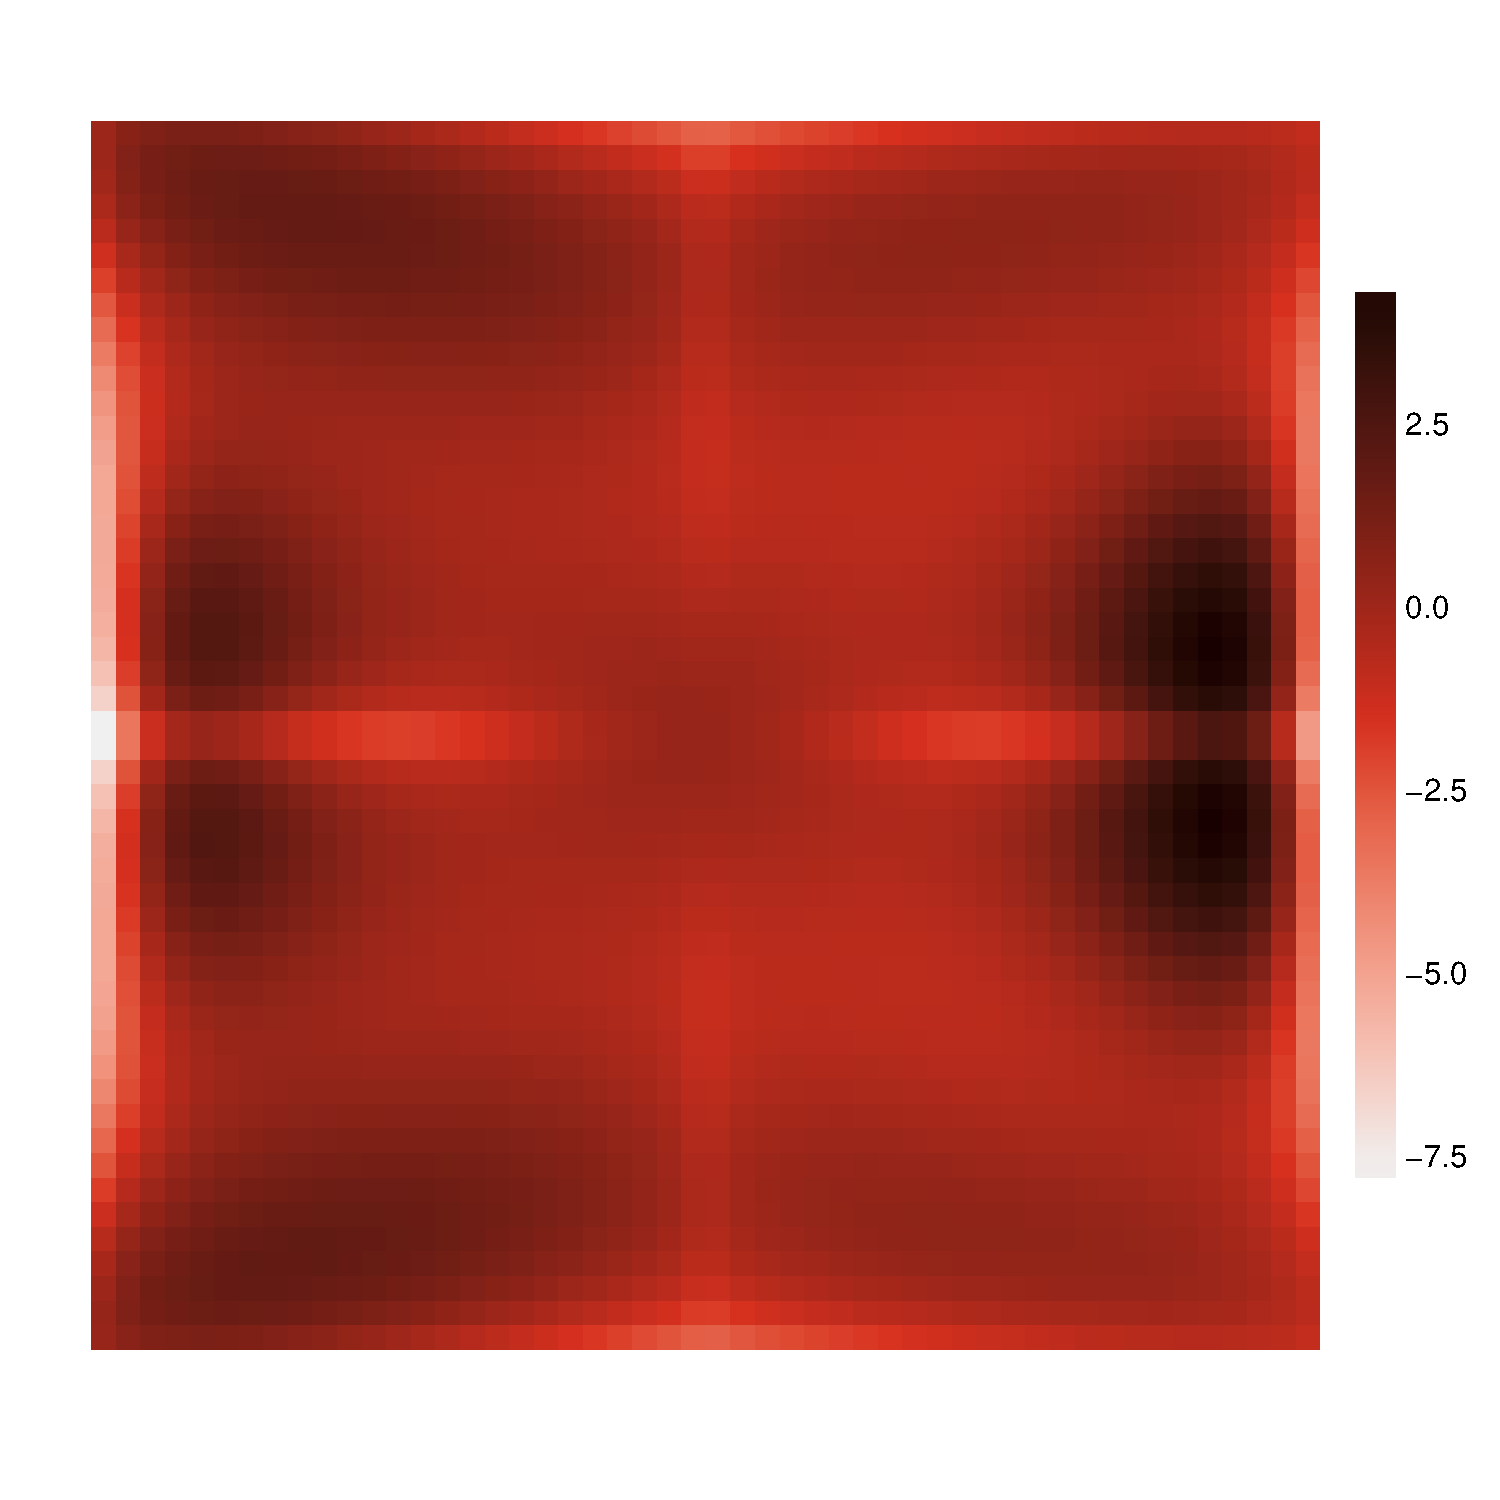
\includegraphics[width=\linewidth]{figures/res114}\\
	\end{subfigure}
	\begin{subfigure}{0.3\textwidth}
		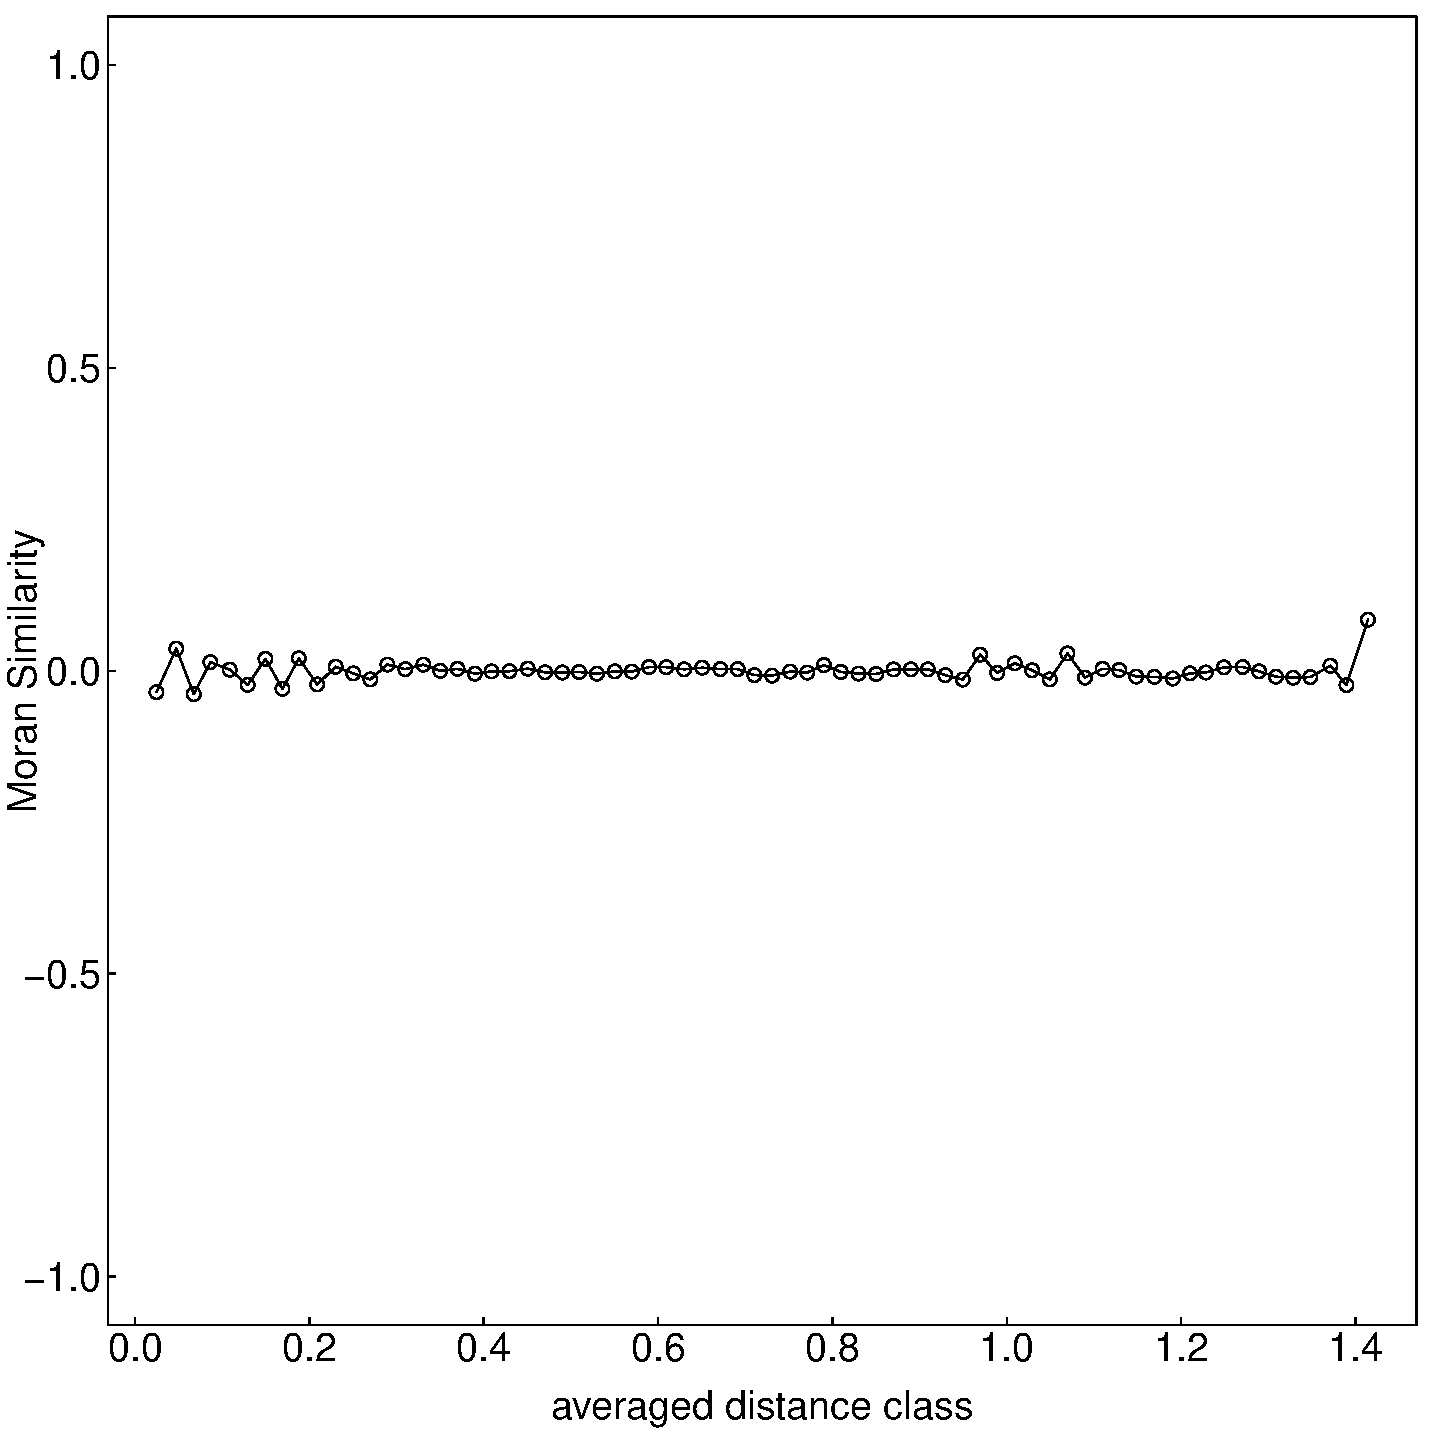
\includegraphics[width=\linewidth]{figures/correlog110}\\
		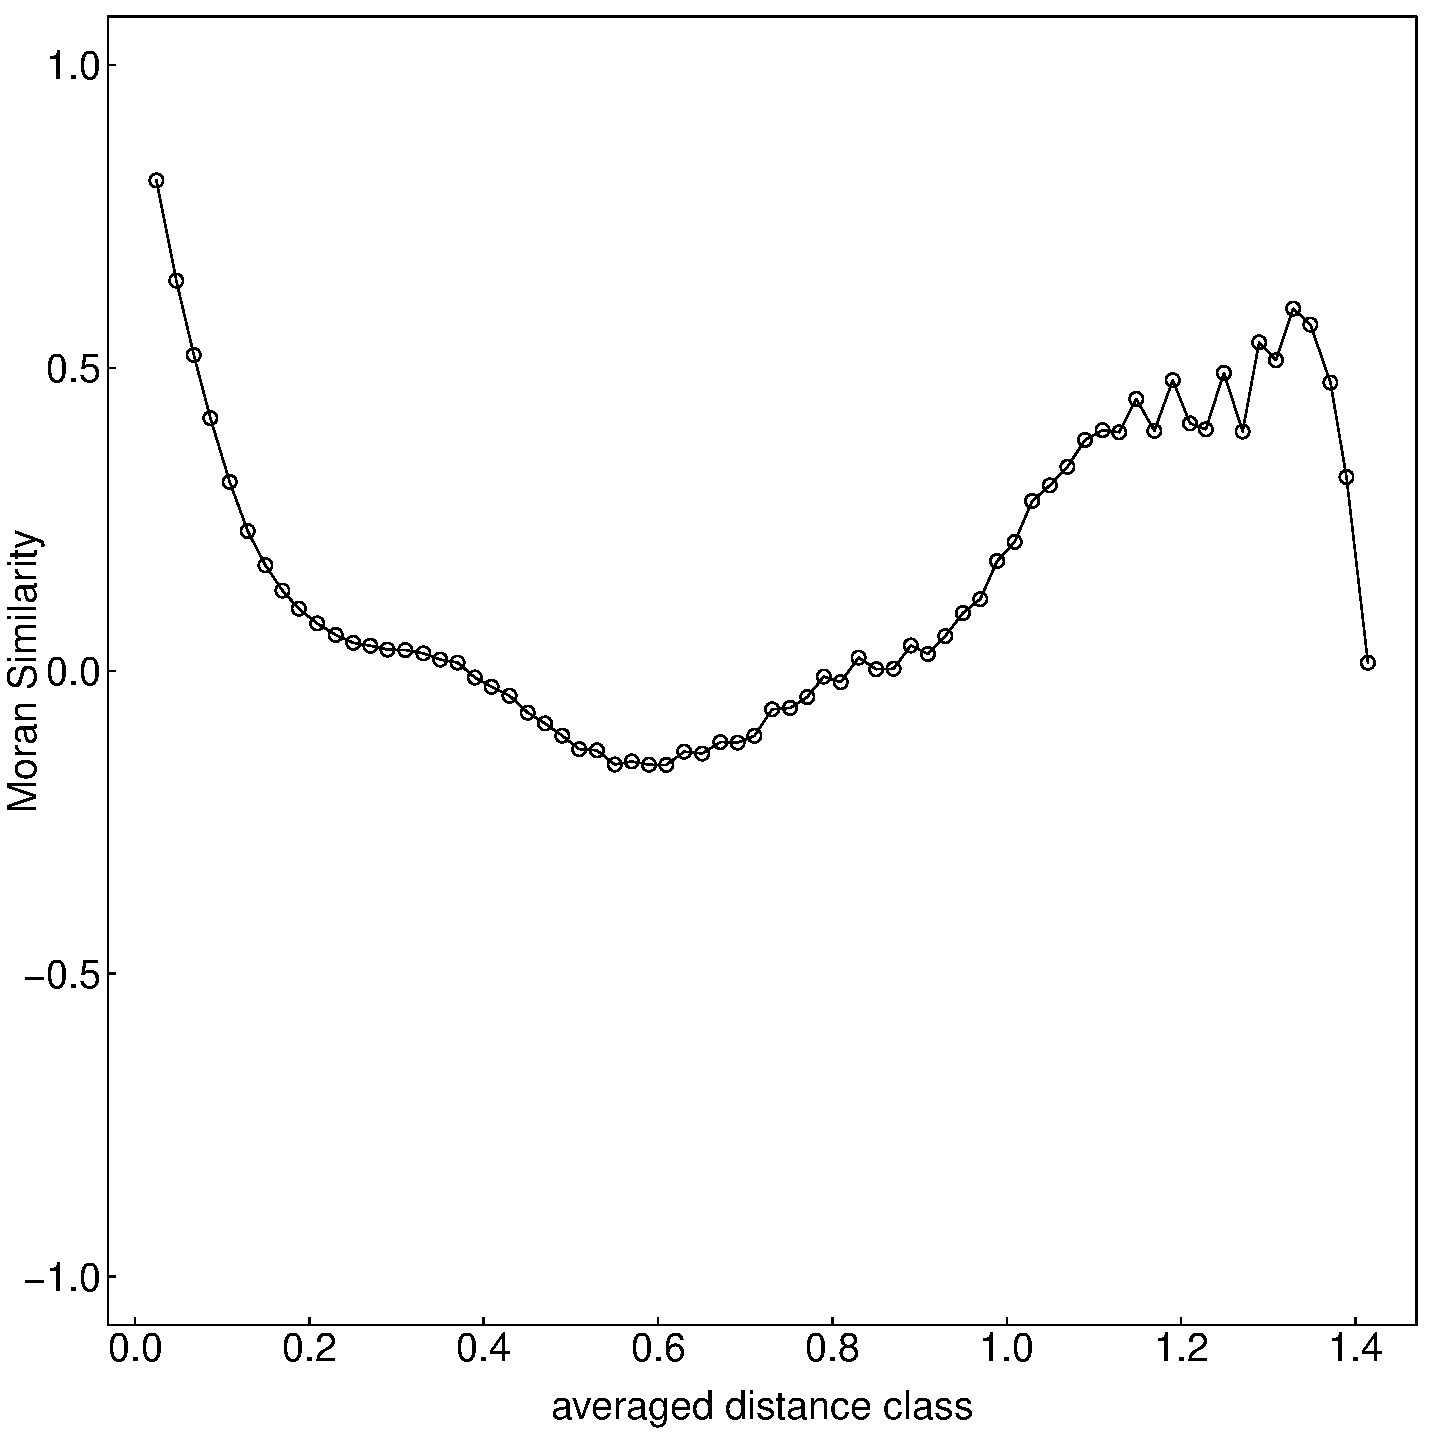
\includegraphics[width=\linewidth]{figures/correlog111}\\
		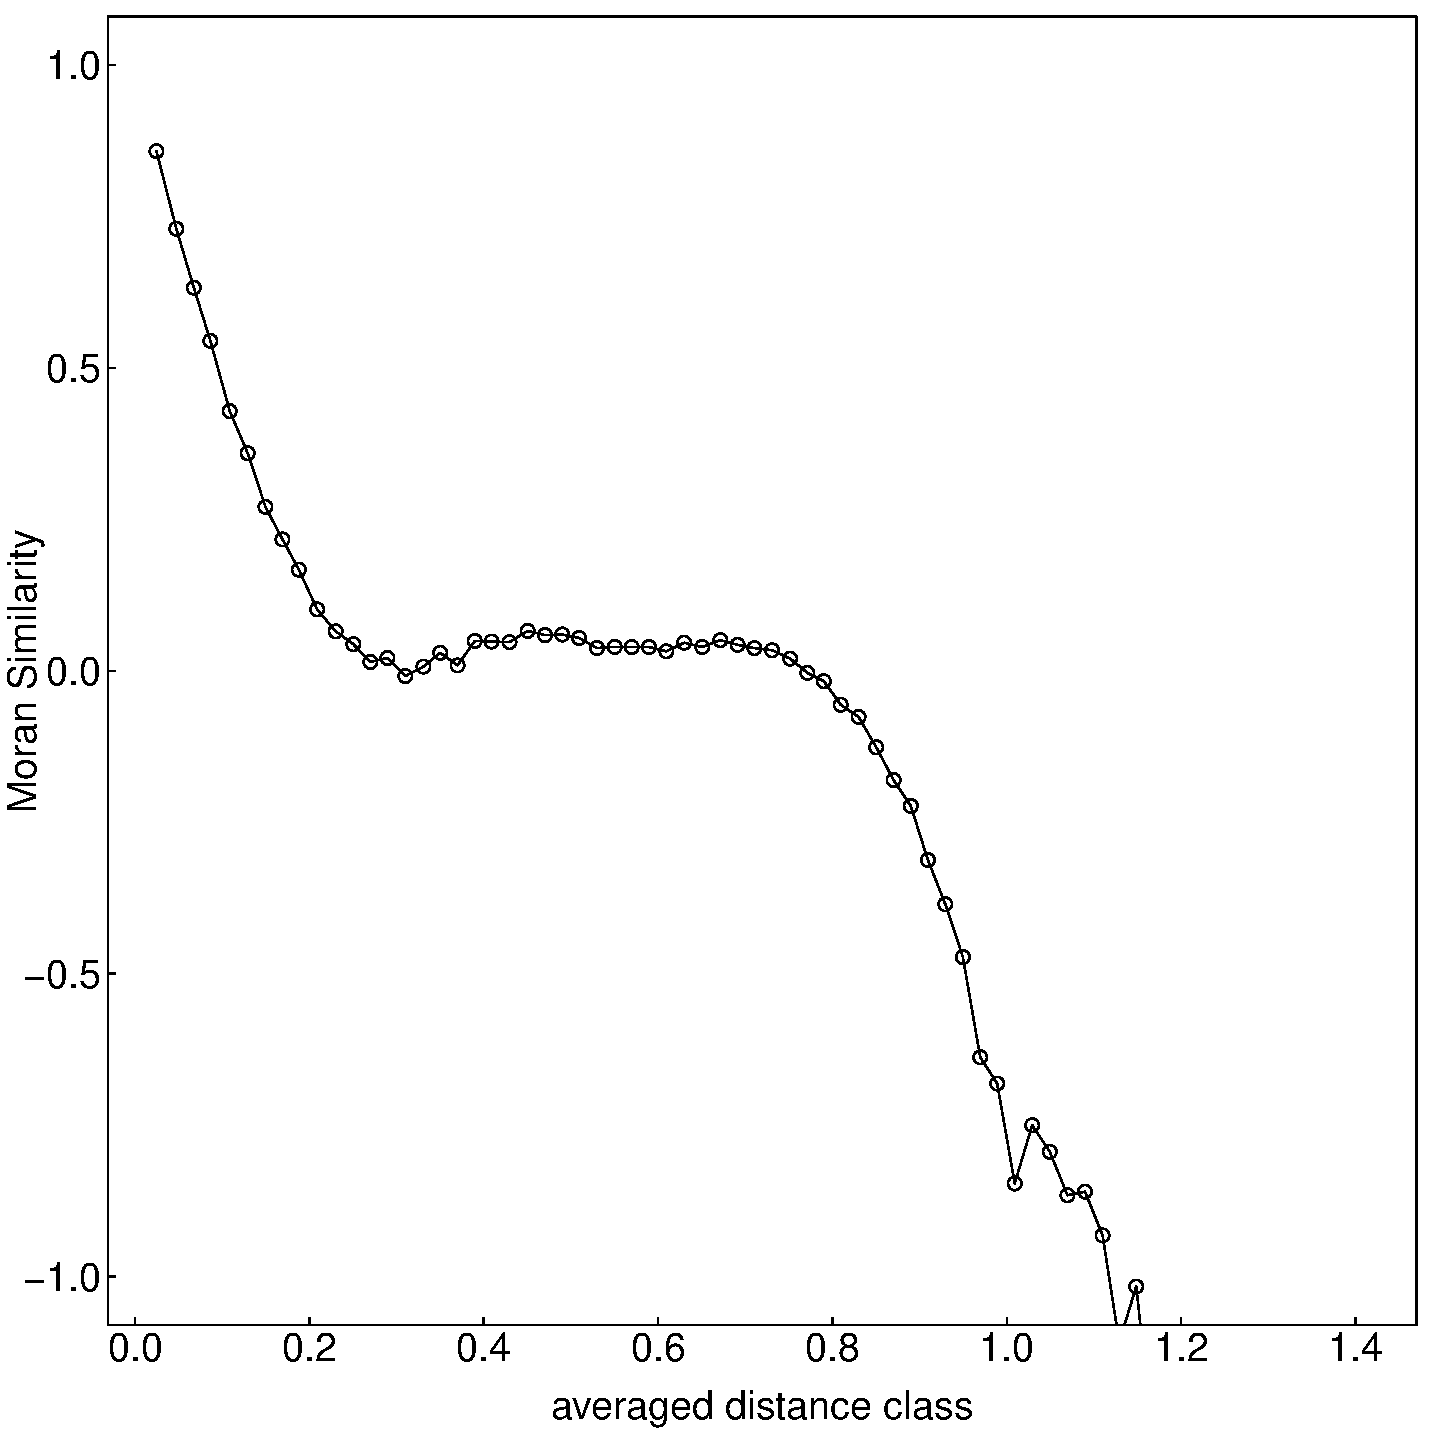
\includegraphics[width=\linewidth]{figures/correlog112}\\
		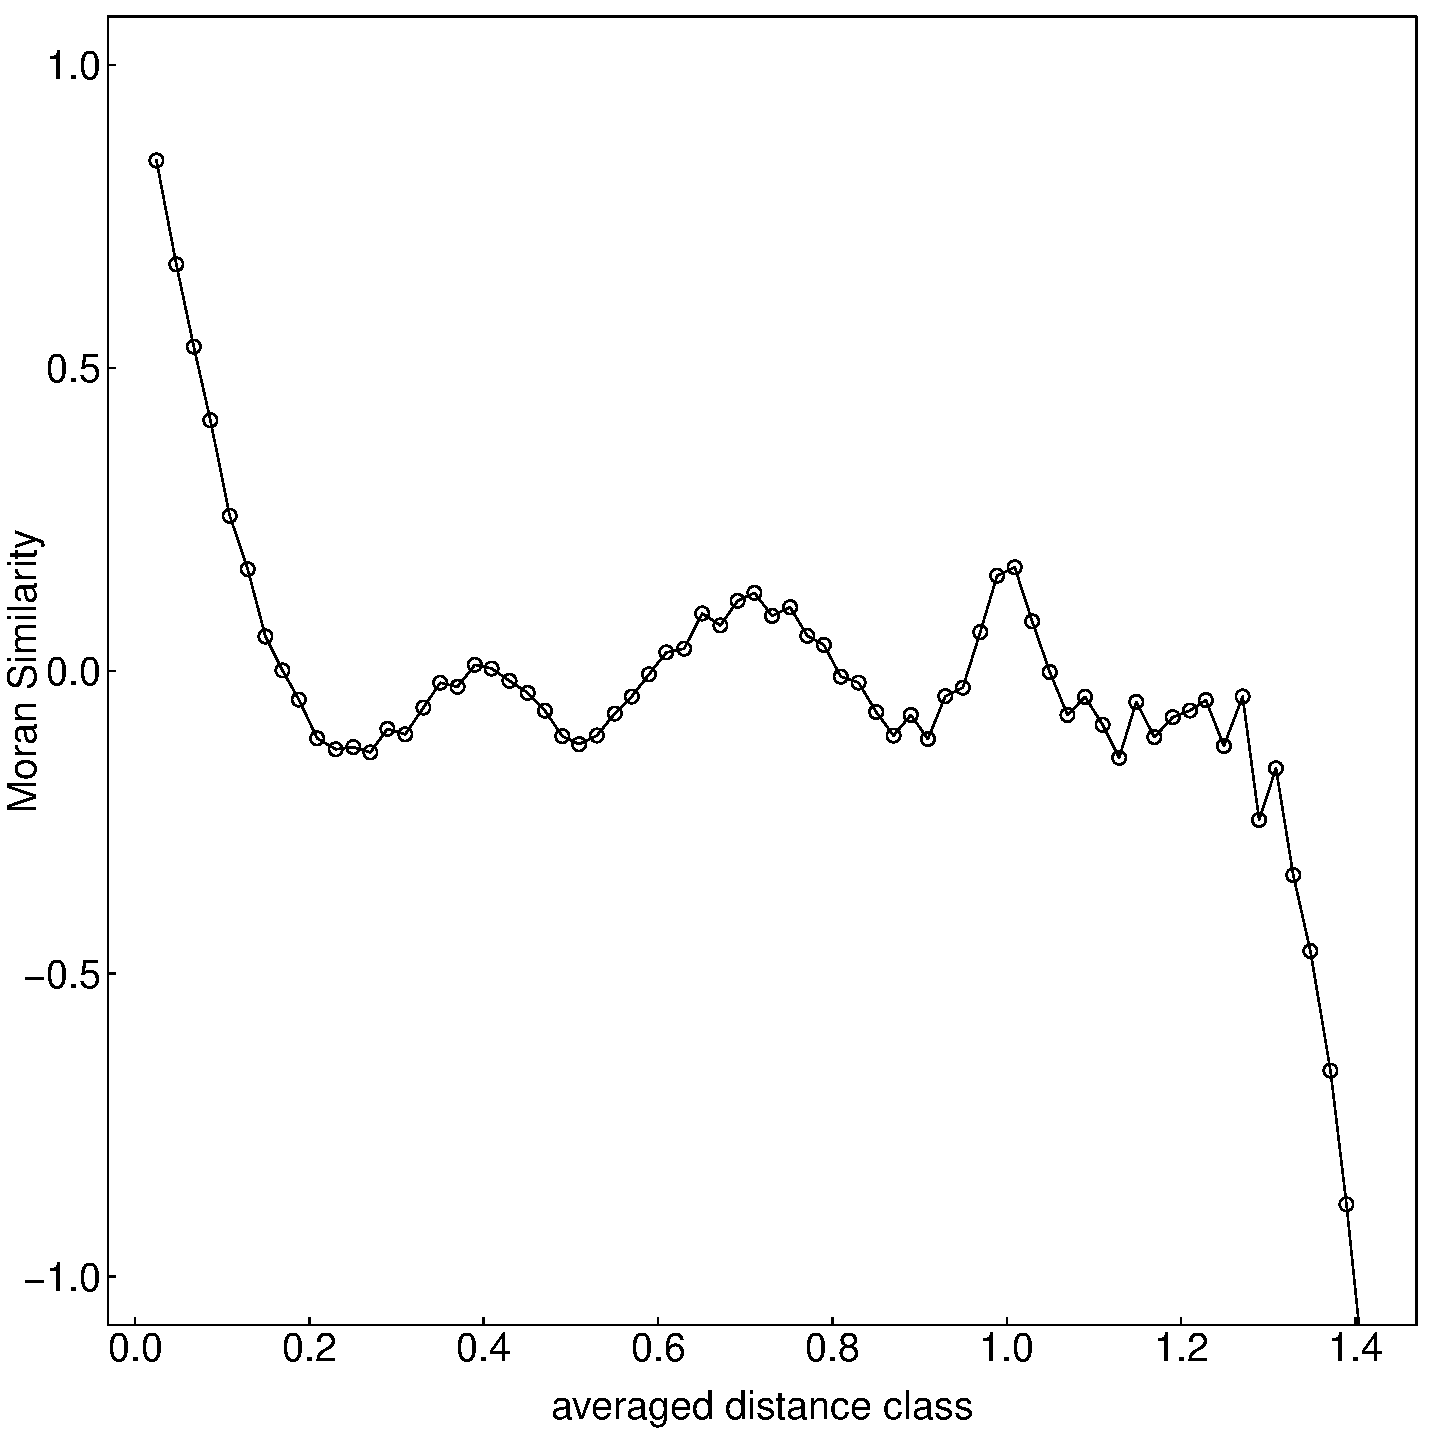
\includegraphics[width=\linewidth]{figures/correlog113}\\
		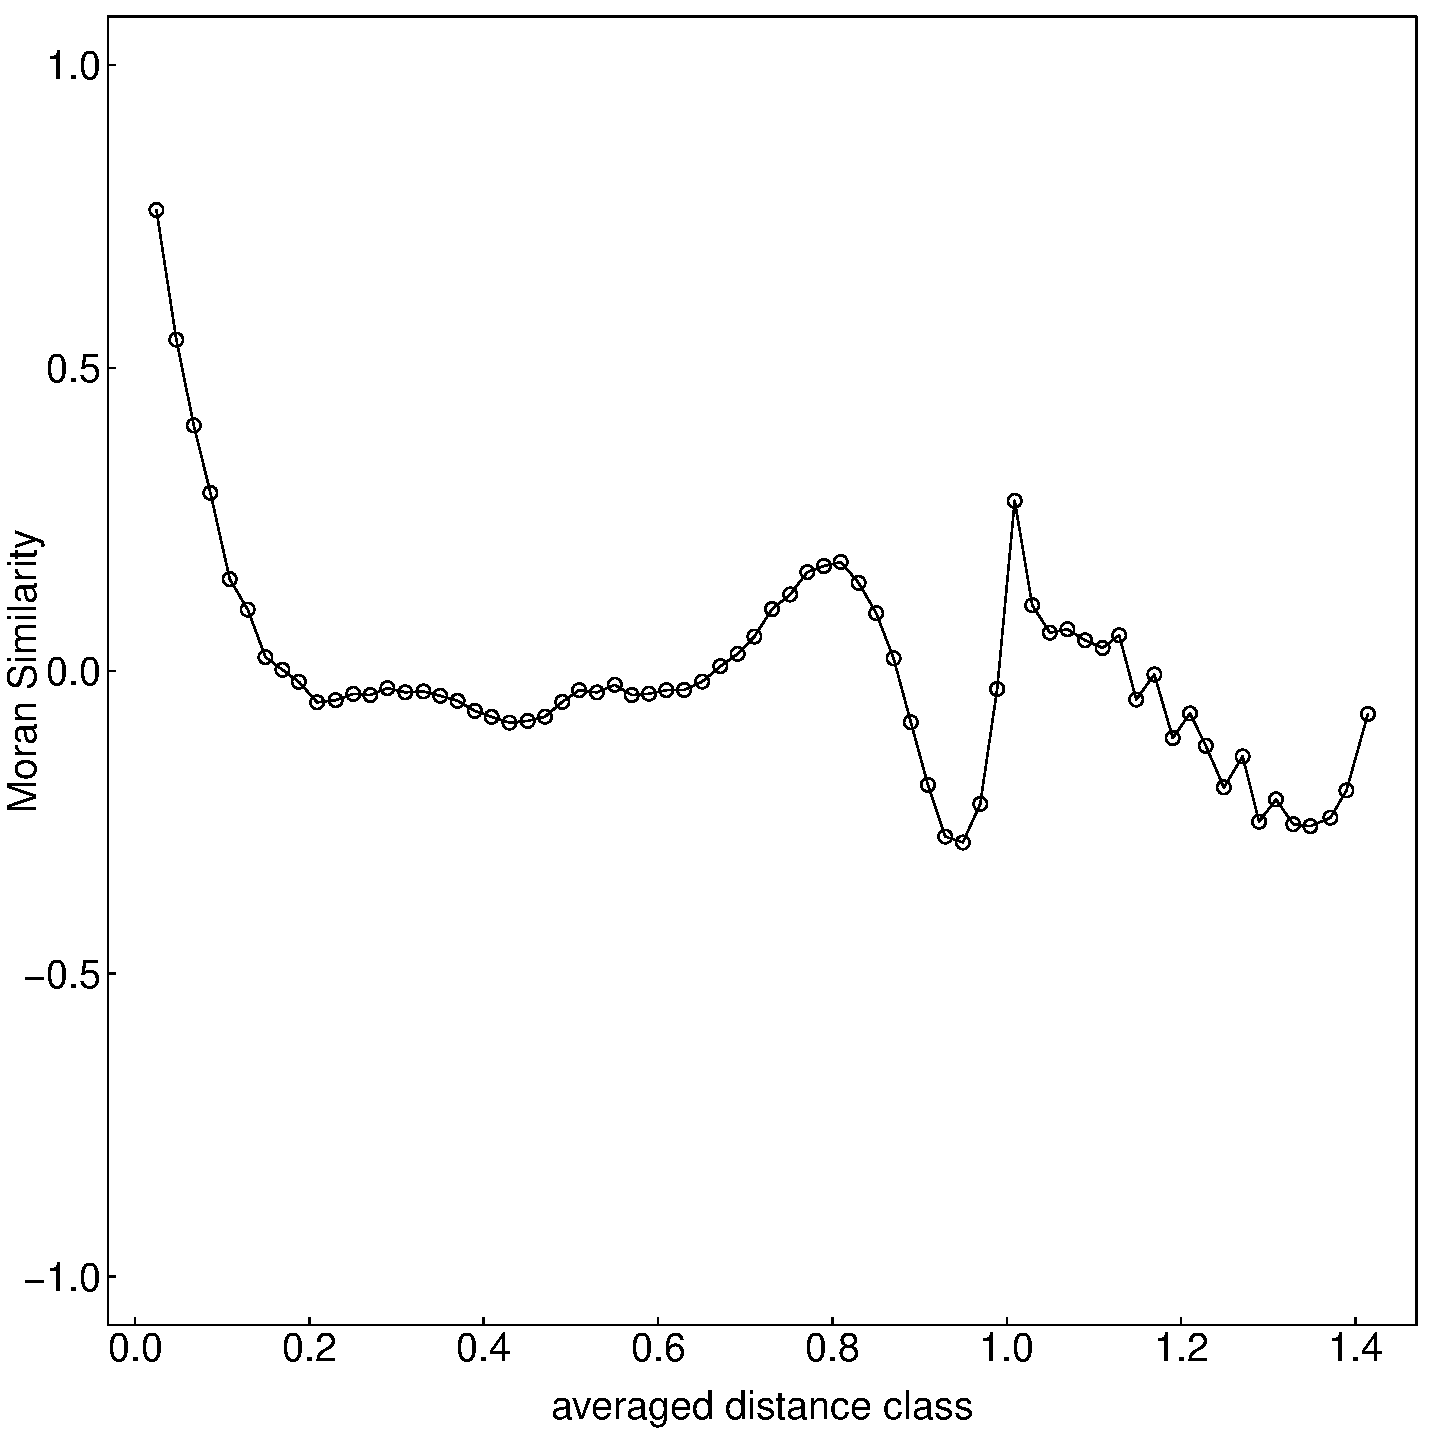
\includegraphics[width=\linewidth]{figures/correlog114}\\
	\end{subfigure}
	\put(-400,375){\Large\textsc{response}}
	\put(-260,375){\Large\textsc{residuals}}
	\put(-110,375){\Large\textsc{correlogram}}
	\put(-500,375){\Large\textsc{SAC cause}}
	\put(-475,355){\Large{0}}
	\put(-475,210){\Large{1}}
	\put(-475,65){\Large{2}}
	\put(-475,-80){\Large{3}}
	\put(-475,-225){\Large{4}}
		\caption{Response and residuals maps and correlograms for smooth landscapes, Gaussian distribution and five different spatial autocorrelation causes. 
			\label{checkSAC}}
\end{figure}
\end{document}